% Options for packages loaded elsewhere
\PassOptionsToPackage{unicode}{hyperref}
\PassOptionsToPackage{hyphens}{url}
%
\documentclass[
]{book}
\usepackage{lmodern}
\usepackage{amssymb,amsmath}
\usepackage{ifxetex,ifluatex}
\ifnum 0\ifxetex 1\fi\ifluatex 1\fi=0 % if pdftex
  \usepackage[T1]{fontenc}
  \usepackage[utf8]{inputenc}
  \usepackage{textcomp} % provide euro and other symbols
\else % if luatex or xetex
  \usepackage{unicode-math}
  \defaultfontfeatures{Scale=MatchLowercase}
  \defaultfontfeatures[\rmfamily]{Ligatures=TeX,Scale=1}
\fi
% Use upquote if available, for straight quotes in verbatim environments
\IfFileExists{upquote.sty}{\usepackage{upquote}}{}
\IfFileExists{microtype.sty}{% use microtype if available
  \usepackage[]{microtype}
  \UseMicrotypeSet[protrusion]{basicmath} % disable protrusion for tt fonts
}{}
\makeatletter
\@ifundefined{KOMAClassName}{% if non-KOMA class
  \IfFileExists{parskip.sty}{%
    \usepackage{parskip}
  }{% else
    \setlength{\parindent}{0pt}
    \setlength{\parskip}{6pt plus 2pt minus 1pt}}
}{% if KOMA class
  \KOMAoptions{parskip=half}}
\makeatother
\usepackage{xcolor}
\IfFileExists{xurl.sty}{\usepackage{xurl}}{} % add URL line breaks if available
\IfFileExists{bookmark.sty}{\usepackage{bookmark}}{\usepackage{hyperref}}
\hypersetup{
  pdftitle={Big Data en R},
  pdfauthor={Alvaro Chirino Gutierrez},
  hidelinks,
  pdfcreator={LaTeX via pandoc}}
\urlstyle{same} % disable monospaced font for URLs
\usepackage{color}
\usepackage{fancyvrb}
\newcommand{\VerbBar}{|}
\newcommand{\VERB}{\Verb[commandchars=\\\{\}]}
\DefineVerbatimEnvironment{Highlighting}{Verbatim}{commandchars=\\\{\}}
% Add ',fontsize=\small' for more characters per line
\usepackage{framed}
\definecolor{shadecolor}{RGB}{248,248,248}
\newenvironment{Shaded}{\begin{snugshade}}{\end{snugshade}}
\newcommand{\AlertTok}[1]{\textcolor[rgb]{0.94,0.16,0.16}{#1}}
\newcommand{\AnnotationTok}[1]{\textcolor[rgb]{0.56,0.35,0.01}{\textbf{\textit{#1}}}}
\newcommand{\AttributeTok}[1]{\textcolor[rgb]{0.77,0.63,0.00}{#1}}
\newcommand{\BaseNTok}[1]{\textcolor[rgb]{0.00,0.00,0.81}{#1}}
\newcommand{\BuiltInTok}[1]{#1}
\newcommand{\CharTok}[1]{\textcolor[rgb]{0.31,0.60,0.02}{#1}}
\newcommand{\CommentTok}[1]{\textcolor[rgb]{0.56,0.35,0.01}{\textit{#1}}}
\newcommand{\CommentVarTok}[1]{\textcolor[rgb]{0.56,0.35,0.01}{\textbf{\textit{#1}}}}
\newcommand{\ConstantTok}[1]{\textcolor[rgb]{0.00,0.00,0.00}{#1}}
\newcommand{\ControlFlowTok}[1]{\textcolor[rgb]{0.13,0.29,0.53}{\textbf{#1}}}
\newcommand{\DataTypeTok}[1]{\textcolor[rgb]{0.13,0.29,0.53}{#1}}
\newcommand{\DecValTok}[1]{\textcolor[rgb]{0.00,0.00,0.81}{#1}}
\newcommand{\DocumentationTok}[1]{\textcolor[rgb]{0.56,0.35,0.01}{\textbf{\textit{#1}}}}
\newcommand{\ErrorTok}[1]{\textcolor[rgb]{0.64,0.00,0.00}{\textbf{#1}}}
\newcommand{\ExtensionTok}[1]{#1}
\newcommand{\FloatTok}[1]{\textcolor[rgb]{0.00,0.00,0.81}{#1}}
\newcommand{\FunctionTok}[1]{\textcolor[rgb]{0.00,0.00,0.00}{#1}}
\newcommand{\ImportTok}[1]{#1}
\newcommand{\InformationTok}[1]{\textcolor[rgb]{0.56,0.35,0.01}{\textbf{\textit{#1}}}}
\newcommand{\KeywordTok}[1]{\textcolor[rgb]{0.13,0.29,0.53}{\textbf{#1}}}
\newcommand{\NormalTok}[1]{#1}
\newcommand{\OperatorTok}[1]{\textcolor[rgb]{0.81,0.36,0.00}{\textbf{#1}}}
\newcommand{\OtherTok}[1]{\textcolor[rgb]{0.56,0.35,0.01}{#1}}
\newcommand{\PreprocessorTok}[1]{\textcolor[rgb]{0.56,0.35,0.01}{\textit{#1}}}
\newcommand{\RegionMarkerTok}[1]{#1}
\newcommand{\SpecialCharTok}[1]{\textcolor[rgb]{0.00,0.00,0.00}{#1}}
\newcommand{\SpecialStringTok}[1]{\textcolor[rgb]{0.31,0.60,0.02}{#1}}
\newcommand{\StringTok}[1]{\textcolor[rgb]{0.31,0.60,0.02}{#1}}
\newcommand{\VariableTok}[1]{\textcolor[rgb]{0.00,0.00,0.00}{#1}}
\newcommand{\VerbatimStringTok}[1]{\textcolor[rgb]{0.31,0.60,0.02}{#1}}
\newcommand{\WarningTok}[1]{\textcolor[rgb]{0.56,0.35,0.01}{\textbf{\textit{#1}}}}
\usepackage{longtable,booktabs}
% Correct order of tables after \paragraph or \subparagraph
\usepackage{etoolbox}
\makeatletter
\patchcmd\longtable{\par}{\if@noskipsec\mbox{}\fi\par}{}{}
\makeatother
% Allow footnotes in longtable head/foot
\IfFileExists{footnotehyper.sty}{\usepackage{footnotehyper}}{\usepackage{footnote}}
\makesavenoteenv{longtable}
\usepackage{graphicx,grffile}
\makeatletter
\def\maxwidth{\ifdim\Gin@nat@width>\linewidth\linewidth\else\Gin@nat@width\fi}
\def\maxheight{\ifdim\Gin@nat@height>\textheight\textheight\else\Gin@nat@height\fi}
\makeatother
% Scale images if necessary, so that they will not overflow the page
% margins by default, and it is still possible to overwrite the defaults
% using explicit options in \includegraphics[width, height, ...]{}
\setkeys{Gin}{width=\maxwidth,height=\maxheight,keepaspectratio}
% Set default figure placement to htbp
\makeatletter
\def\fps@figure{htbp}
\makeatother
\setlength{\emergencystretch}{3em} % prevent overfull lines
\providecommand{\tightlist}{%
  \setlength{\itemsep}{0pt}\setlength{\parskip}{0pt}}
\setcounter{secnumdepth}{5}

\title{Big Data en R}
\usepackage{etoolbox}
\makeatletter
\providecommand{\subtitle}[1]{% add subtitle to \maketitle
  \apptocmd{\@title}{\par {\large #1 \par}}{}{}
}
\makeatother
\subtitle{EST-383}
\author{Alvaro Chirino Gutierrez}
\date{2021-03-23}

\begin{document}
\maketitle

{
\setcounter{tocdepth}{1}
\tableofcontents
}
\hypertarget{prefacio}{%
\chapter*{Prefacio}\label{prefacio}}
\addcontentsline{toc}{chapter}{Prefacio}

Este documento de \href{https://twiiter/alvarochirinog}{Alvaro Chirino} esta bajo la licencia de Creative Commons Attribution-NonCommercial-ShareAlike 4.0 International License.

\hypertarget{audiencia}{%
\section*{Audiencia}\label{audiencia}}
\addcontentsline{toc}{section}{Audiencia}

El libro fue diseñado originalmente para los estudiantes de la materia de Programación Estadística I, una materia optativa del pregrado de la carrera de Estadística de la Universidad Mayor de San Andres.

Este documento representa un primer acercamiento a los estudiantes de estadistica al software R y al mundo del Big Data.

\hypertarget{estructura-del-libro}{%
\section*{Estructura del libro}\label{estructura-del-libro}}
\addcontentsline{toc}{section}{Estructura del libro}

El libro inluye 5 capitulos, estos son:

\begin{enumerate}
\def\labelenumi{\arabic{enumi}.}
\tightlist
\item
  Introducción a R
\item
  Scraping Web en R
\item
  Introducción al Big Data
\item
  Big Data en R
\item
  R y Spark
\end{enumerate}

\hypertarget{software-y-acuerdos}{%
\section*{Software y acuerdos}\label{software-y-acuerdos}}
\addcontentsline{toc}{section}{Software y acuerdos}

\begin{Shaded}
\begin{Highlighting}[]
\KeywordTok{sessionInfo}\NormalTok{()}
\end{Highlighting}
\end{Shaded}

\begin{verbatim}
## R version 4.0.4 (2021-02-15)
## Platform: x86_64-w64-mingw32/x64 (64-bit)
## Running under: Windows 10 x64 (build 19042)
## 
## Matrix products: default
## 
## locale:
## [1] LC_COLLATE=Spanish_Bolivia.1252 
## [2] LC_CTYPE=Spanish_Bolivia.1252   
## [3] LC_MONETARY=Spanish_Bolivia.1252
## [4] LC_NUMERIC=C                    
## [5] LC_TIME=Spanish_Bolivia.1252    
## 
## attached base packages:
## [1] stats     graphics  grDevices utils    
## [5] datasets  methods   base     
## 
## other attached packages:
## [1] dplyr_1.0.5
## 
## loaded via a namespace (and not attached):
##  [1] rstudioapi_0.13   knitr_1.31       
##  [3] magrittr_2.0.1    tidyselect_1.1.0 
##  [5] R6_2.5.0          rlang_0.4.10     
##  [7] stringr_1.4.0     highr_0.8        
##  [9] tools_4.0.4       packrat_0.5.0    
## [11] xfun_0.19         DBI_1.1.1        
## [13] htmltools_0.5.1.1 ellipsis_0.3.1   
## [15] assertthat_0.2.1  yaml_2.2.1       
## [17] digest_0.6.27     tibble_3.0.6     
## [19] lifecycle_1.0.0   crayon_1.4.1     
## [21] bookdown_0.21     purrr_0.3.4      
## [23] vctrs_0.3.6       rsconnect_0.8.16 
## [25] glue_1.4.2        evaluate_0.14    
## [27] rmarkdown_2.6     stringi_1.5.3    
## [29] compiler_4.0.4    pillar_1.4.7     
## [31] generics_0.1.0    pkgconfig_2.0.3
\end{verbatim}

\hypertarget{bases-de-datos}{%
\section*{Bases de datos}\label{bases-de-datos}}
\addcontentsline{toc}{section}{Bases de datos}

En este documento se emplearan 4 bases de datos del contecto Boliviano:

\begin{enumerate}
\def\labelenumi{\arabic{enumi}.}
\tightlist
\item
  Encuesta a Hogares 2019 y 2019. Vivienda y Personas
\item
  Encuesta de Demografía y Salud 1989 - 2008
\item
  Encuesta de Niños, niñas y adolescentes 2016
\item
  Computo oficial de las elecciones del 20 de Octubre de 2019
\item
  Bases de datos de contagios, muertes y recuperados del COVID-19 del Johns Hopkins Institute.
\end{enumerate}

Estas bases de datos se encuentran disponibles en formato \(.RData\) en el repositorio de Github del texto.

\hypertarget{agradecimiento}{%
\section*{Agradecimiento}\label{agradecimiento}}
\addcontentsline{toc}{section}{Agradecimiento}

Eponine\ldots{}

\hypertarget{introR}{%
\chapter{Introducción a R}\label{introR}}

\begin{quote}
R es un software de libre distribución
\end{quote}

\hypertarget{quuxe9-es-r}{%
\section{¿Qué es R?}\label{quuxe9-es-r}}

\begin{figure}
\centering
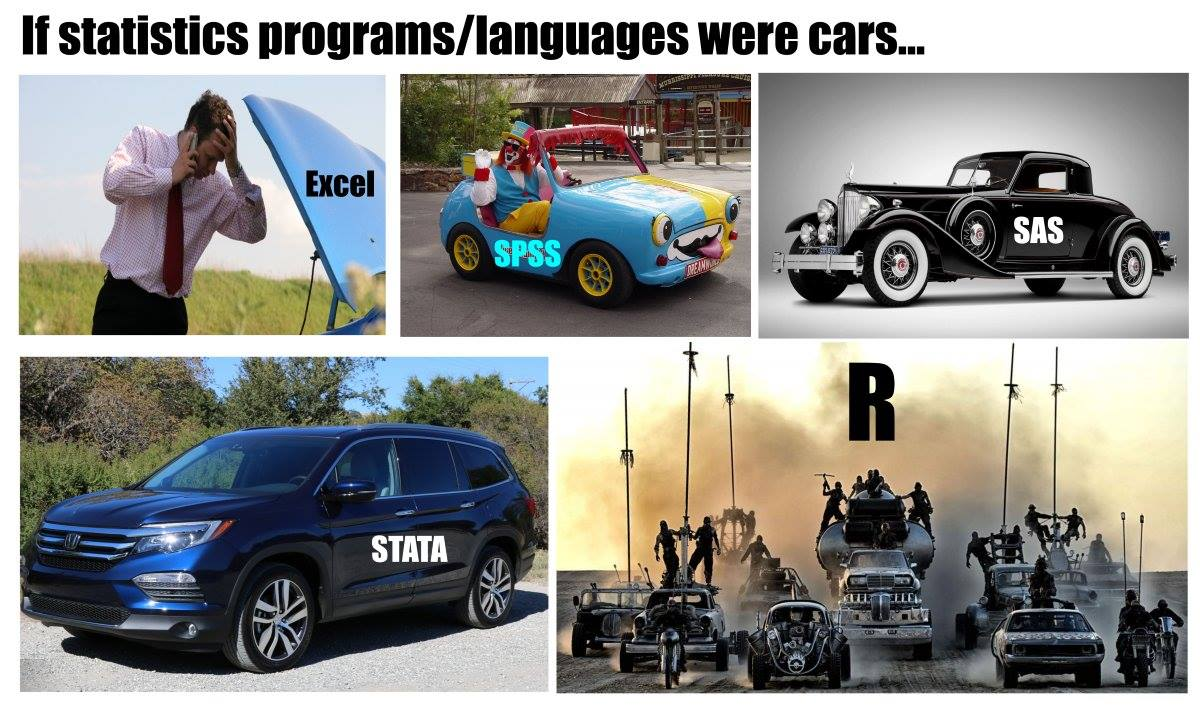
\includegraphics{images/r.jpg}
\caption{Comparación perfecta}
\end{figure}

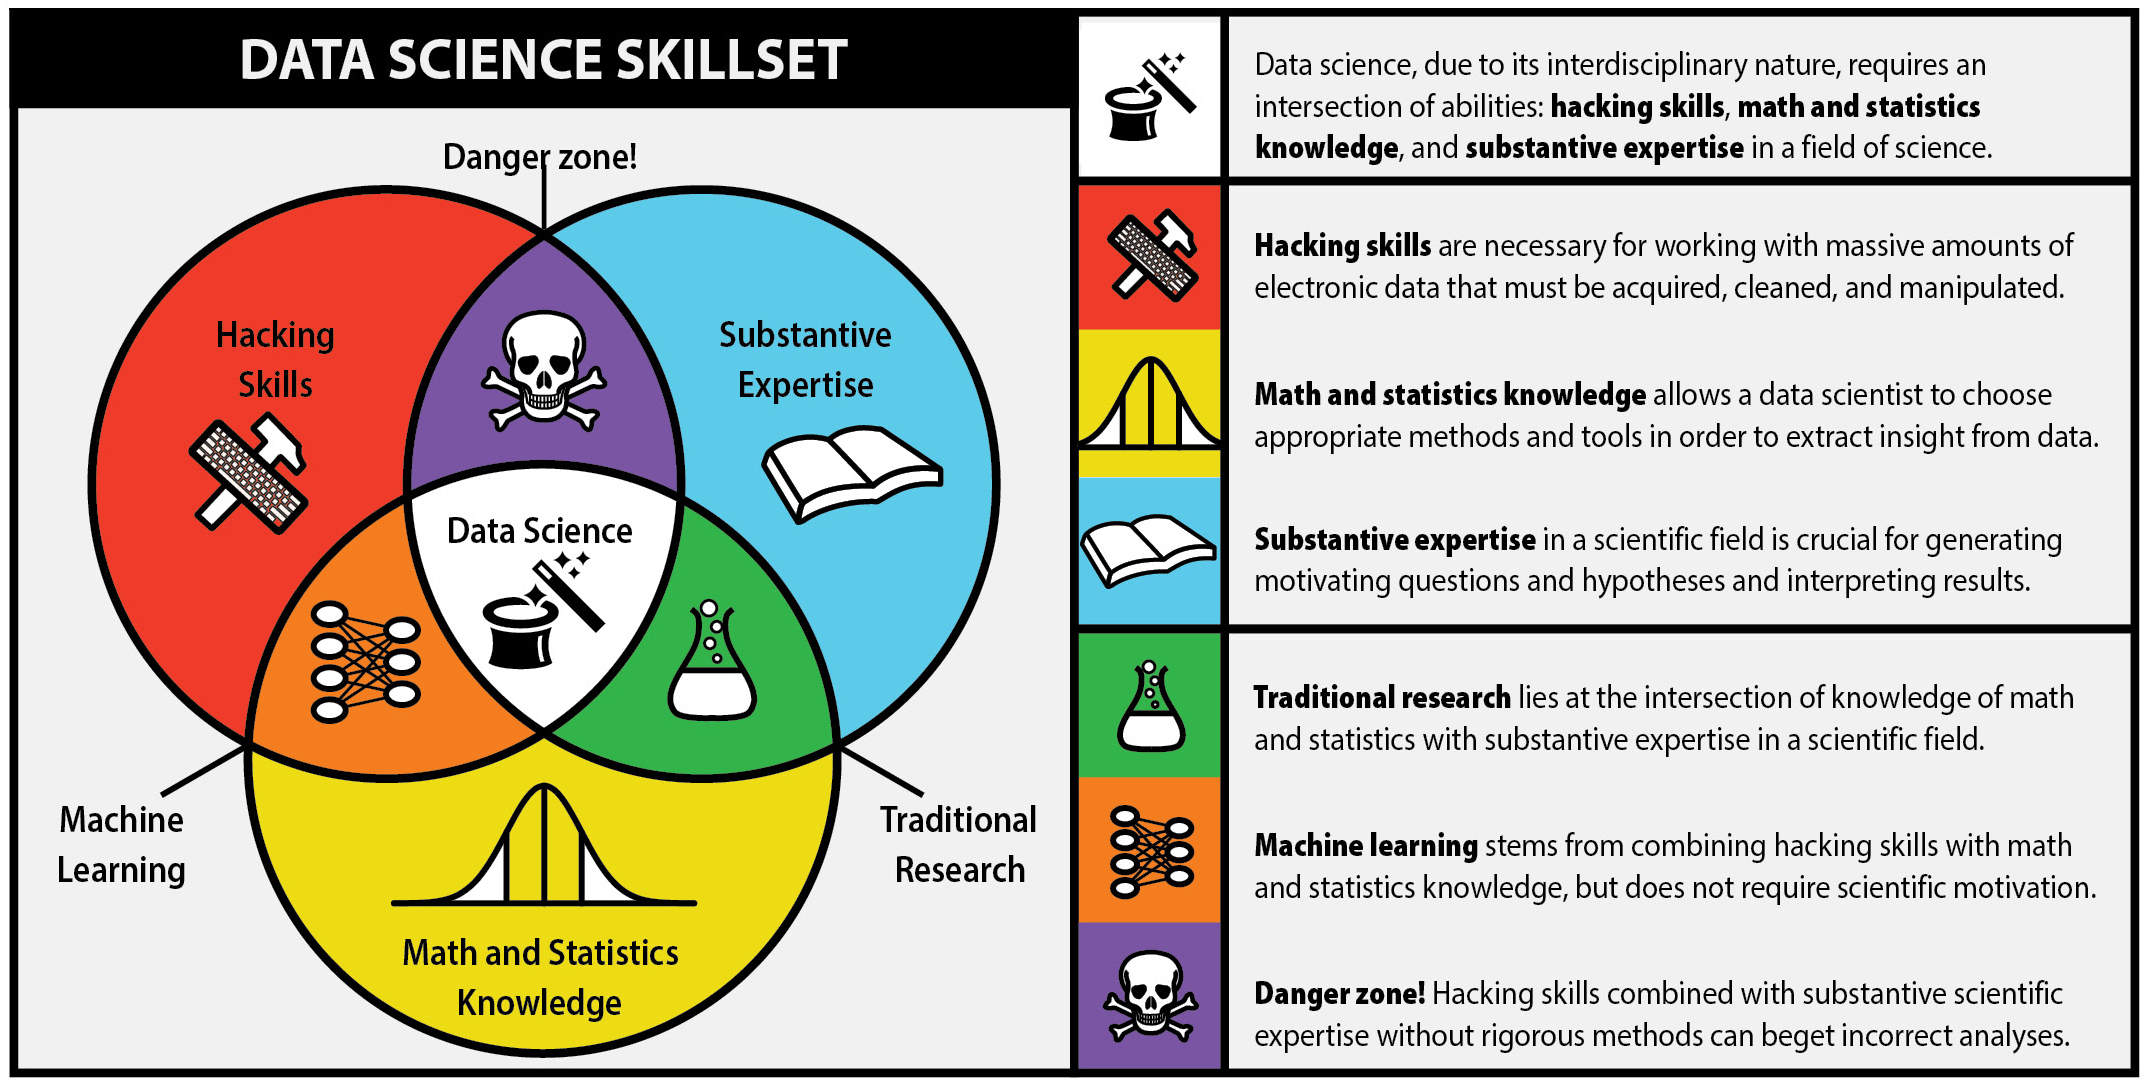
\includegraphics{images/ds.jpg}
\#\#\# Algo de historia de R

\begin{itemize}
\tightlist
\item
  R es el hermano de S
\item
  S es un lenguaje de programación estadística desarrollado por John Chambers de Bell Labs
\item
  El objetivo de S era ``convertir las ideas en el software, de forma rápida y fielmente''
\item
  S fue creado en 1976 y se reinvento 1988 introduciendo muchos cambios
\item
  En 1993, StatSci (fabricante de S-Plus) adquieren licencia exclusiva a S
\item
  S-Plus integra S con una interfaz gráfica de usuario agradable y pleno apoyo al cliente
\item
  R Fue creado por Ross Ihaka y Robert Gentleman de la University of Auckland, New Zealand
\end{itemize}

\hypertarget{acerca-de-r}{%
\subsection{Acerca de R}\label{acerca-de-r}}

\begin{itemize}
\tightlist
\item
  El proyecto R inicio en 1991
\item
  R apareció por primera vez en 1996 como un software de código abierto!
\item
  Altamente personalizable a través de paquetes
\item
  La comunidad R, se basa en el poder de la colaboración con miles de paquetes de libre disposición
\item
  Existen muchas interfaces gráficas de usuario de R libres y comerciales (por ejemplo R Studio y Revolución)
\end{itemize}

\hypertarget{quuxe9-es-r-1}{%
\subsection{¿Qué es R?}\label{quuxe9-es-r-1}}

R es un conjunto integrado de servicios de software para la manipulación de datos, cálculo y representación gráfica. Incluye:

\begin{itemize}
\tightlist
\item
  instalación sencilla y un fácil almacenamiento de datos
\item
  un conjunto de operadores para los cálculos en arrays, particularmente en las matrices
\item
  facilidad en los gráficos y el análisis de datos y
\item
  bien desarrollado, lenguaje de programación sencillo y eficaz que incluye condicionales, bucles, funciones recursivas definidos por el usuario.
\item
  Altamente intuitivo
\end{itemize}

\begin{quote}
A pesar de ser libre y de código abierto, R es ampliamente utilizado por los analistas de datos dentro de las empresas y el mundo académico. (R en the NY Times)
\end{quote}

Ver \href{https://www.nytimes.com/2009/01/07/technology/business-computing/07program.html?pagewanted=all\&_r=0}{NY Times} artículo.

\hypertarget{algunas-referencias}{%
\subsection{Algunas referencias}\label{algunas-referencias}}

\begin{itemize}
\tightlist
\item
  aRrgh: a newcomer's (angry) guide to R by Tim Smith and Kevin Ushey
\item
  Introductory Statistics with by Peter Dalgaard
\item
  R tarjeta de comandos \url{http://cran.r-project.org/doc/contrib/Short-refcard.pdf}
\item
  Tutorial de R \url{http://www.cyclismo.org/tutorial/R/}
\item
  R project and Bioconductor
\end{itemize}

Mas avanzado:

\begin{itemize}
\tightlist
\item
  Hadley Wickham's book
\end{itemize}

\hypertarget{rstudio}{%
\subsection{RStudio}\label{rstudio}}

RStudio es un ambiente libre y abierto de desarrollo de código integrado.

\begin{itemize}
\tightlist
\item
  multiplataforma
\item
  El resaltado de sintaxis, completado de código, y la sangría inteligente
\item
  gestionar fácilmente múltiples directorios de trabajo
\item
  Flexible para el manejo de gráficos
\item
  Integrado con Knitr
\item
  Integrado con Git
\end{itemize}

\hypertarget{instalaciuxf3n}{%
\subsection{Instalación}\label{instalaciuxf3n}}

\begin{itemize}
\tightlist
\item
  R-CRAN \url{https://cran.r-project.org/} (elija el Sistema operativo, descargue y siguiente, siguiente\ldots)
\item
  R-Studio \url{https://www.rstudio.com/} (elija el Sistema operativo, descargue y siguiente, siguiente\ldots)
\end{itemize}

Nota: Para actualizar ambos paquetes: descargue la nueva versión e instale (las librerías no sufren cambios).

\hypertarget{r-markdown}{%
\section{R Markdown}\label{r-markdown}}

\textbf{``R Markdown''} se introdujo por primera vez en el paquete knitr a principios de 2012. La idea era incrustar fragmentos de código (de R u otros) en los documentos de Markdown. De hecho, knitr soportó varios lenguajes de autoría desde el principio además de Markdown, incluidos LaTeX, HTML, AsciiDoc, reStructuredText y Textile.

Markdown se ha convertido en el formato de documento más popular. La simplicidad de Markdown se destaca claramente entre estos formatos de documentos.

\hypertarget{instalaciuxf3n-1}{%
\subsection{Instalación}\label{instalaciuxf3n-1}}

\begin{Shaded}
\begin{Highlighting}[]
\KeywordTok{install.packages}\NormalTok{(}\StringTok{'rmarkdown'}\NormalTok{)}

\CommentTok{# Si se prefiere la versión en desarrollo}
\ControlFlowTok{if}\NormalTok{ (}\OperatorTok{!}\KeywordTok{requireNamespace}\NormalTok{(}\StringTok{"devtools"}\NormalTok{))}
  \KeywordTok{install.packages}\NormalTok{(}\StringTok{'devtools'}\NormalTok{)}
\NormalTok{devtools}\OperatorTok{::}\KeywordTok{install_github}\NormalTok{(}\StringTok{'rstudio/rmarkdown'}\NormalTok{)}
\end{Highlighting}
\end{Shaded}

Si el objetivo es usar Markdown para generar documentos PDF se necesita instalar Latex.

Existen cheatsheets utiles para usar markdown, como: \href{https://github.com/rstudio/cheatsheets/raw/master/rmarkdown-2.0.pdf}{cheatsheets}

\hypertarget{yaml-header}{%
\subsection{YAML Header}\label{yaml-header}}

Al inicio del archivo y entre las lineas ---

\begin{Shaded}
\begin{Highlighting}[]
\OperatorTok{---}
\NormalTok{title}\OperatorTok{:}\StringTok{ }\NormalTok{Mi documento}
\NormalTok{author}\OperatorTok{:}\StringTok{ }\NormalTok{Juan Perez}
\NormalTok{date}\OperatorTok{:}\StringTok{ }\NormalTok{Marzo }\DecValTok{22}\NormalTok{, }\DecValTok{20220}
\NormalTok{output}\OperatorTok{:}\StringTok{ }\NormalTok{html_document}
\OperatorTok{---}
\end{Highlighting}
\end{Shaded}

\hypertarget{sintaxis-buxe1sica}{%
\subsection{Sintaxis básica}\label{sintaxis-buxe1sica}}

Énfasis sobre el texto,

\begin{Shaded}
\begin{Highlighting}[]
\OperatorTok{*}\NormalTok{italic}\OperatorTok{*}\StringTok{   }\ErrorTok{**}\NormalTok{bold}\OperatorTok{**}
\NormalTok{_italic_   __bold__}
\end{Highlighting}
\end{Shaded}

Secciones,

\begin{Shaded}
\begin{Highlighting}[]
\CommentTok{# Header 1}
\CommentTok{## Header 2}
\CommentTok{### Header 3}
\end{Highlighting}
\end{Shaded}

Items (viñetas) no ordenadas y ordenadas,

\begin{Shaded}
\begin{Highlighting}[]
\OperatorTok{*}\StringTok{ }\NormalTok{Item }\DecValTok{1}
\OperatorTok{*}\StringTok{ }\NormalTok{Item }\DecValTok{2}
    \OperatorTok{+}\StringTok{ }\NormalTok{Item 2a}
    \OperatorTok{+}\StringTok{ }\NormalTok{Item 2b}

\FloatTok{1.}\NormalTok{ Item }\DecValTok{1}
\FloatTok{2.}\NormalTok{ Item }\DecValTok{2}
\FloatTok{3.}\NormalTok{ Item }\DecValTok{3}
    \OperatorTok{+}\StringTok{ }\NormalTok{Item 3a}
    \OperatorTok{+}\StringTok{ }\NormalTok{Item 3b}
\end{Highlighting}
\end{Shaded}

Palabras clave con referencias web,

\begin{Shaded}
\begin{Highlighting}[]
\NormalTok{[linked phrase](http}\OperatorTok{:}\ErrorTok{//}\NormalTok{example.com)}
\end{Highlighting}
\end{Shaded}

Imágenes simples o con titulo,

\begin{Shaded}
\begin{Highlighting}[]
\OperatorTok{!}\NormalTok{[](http}\OperatorTok{:}\ErrorTok{//}\NormalTok{example.com}\OperatorTok{/}\NormalTok{logo.png)}

\OperatorTok{!}\NormalTok{[optional caption text](figures}\OperatorTok{/}\NormalTok{img.png)}
\end{Highlighting}
\end{Shaded}

Blockquotes

\begin{quote}
It's always better to give than to receive.
\end{quote}

\begin{Shaded}
\begin{Highlighting}[]
\NormalTok{A friend once said}\OperatorTok{:}

\ErrorTok{>}\StringTok{ }\NormalTok{It}\StringTok{'s always better to give than to receive.}
\end{Highlighting}
\end{Shaded}

Ecuaciones en linea y en párrafo,

En linea \(\sum_i{x^2}\) o en párrafo:

\[\sum_i{x^2}\]

\begin{Shaded}
\begin{Highlighting}[]
\OperatorTok{$}\NormalTok{equation}\OperatorTok{$}

\ErrorTok{$$}\StringTok{ }\NormalTok{equation }\OperatorTok{$}\ErrorTok{$}
\end{Highlighting}
\end{Shaded}

\hypertarget{tipos-de-documentos}{%
\subsection{Tipos de documentos}\label{tipos-de-documentos}}

\begin{itemize}
\tightlist
\item
  beamer\_presentation
\item
  github\_document
\item
  html\_document
\item
  ioslides\_presentation
\item
  latex\_document
\item
  md\_document
\item
  odt\_document
\item
  pdf\_document
\item
  powerpoint\_presentation
\item
  rtf\_document
\item
  slidy\_presentation
\item
  word\_document
\end{itemize}

\hypertarget{chunks}{%
\subsection{Chunks}\label{chunks}}

Los chunks son entornos que permiten incluir código en R dentro de las distintos tipos de documentos que genera Rmarkdown, los chunks inician con \texttt{\textasciigrave{}\textasciigrave{}\textasciigrave{}\{r\}\ y\ termina\ con\ \textasciigrave{}\textasciigrave{}\textasciigrave{}}, también es posible introducir chunks en linea con el texto, esto se logra introduciendo

\begin{Shaded}
\begin{Highlighting}[]
\NormalTok{Texto ... }\StringTok{`}\DataTypeTok{r <code>}\StringTok{`}\NormalTok{ ... texto}
\end{Highlighting}
\end{Shaded}

La parte \{r\} del chunk sirve para introducir las distintas opciones que va a contener ese chunk, las opciones disponibles son:

\begin{itemize}
\tightlist
\item
  echo (default = TRUE), muestra el código del chunk en la salida del documento
\item
  eval (default = TRUE), corre el código del chunk
\item
  message (default = TRUE), muestra los mensajes que genera el chunk
\end{itemize}

Existen funciones útiles para mejorar las salidas de tablas, tales como xtable y kable de la librería knitr.

\hypertarget{r-buxe1sico}{%
\section{R básico}\label{r-buxe1sico}}

R es una calculadora demasiado grande

\begin{Shaded}
\begin{Highlighting}[]
\DecValTok{123}\OperatorTok{+}\DecValTok{456}
\end{Highlighting}
\end{Shaded}

\begin{verbatim}
## [1] 579
\end{verbatim}

\begin{Shaded}
\begin{Highlighting}[]
\DecValTok{4657}\OperatorTok{*}\DecValTok{89}
\end{Highlighting}
\end{Shaded}

\begin{verbatim}
## [1] 414473
\end{verbatim}

\begin{Shaded}
\begin{Highlighting}[]
\DecValTok{12}\OperatorTok{/}\DecValTok{34}
\end{Highlighting}
\end{Shaded}

\begin{verbatim}
## [1] 0.3529412
\end{verbatim}

\begin{Shaded}
\begin{Highlighting}[]
\DecValTok{2443-3434}
\end{Highlighting}
\end{Shaded}

\begin{verbatim}
## [1] -991
\end{verbatim}

\hypertarget{luxf3gica-de-los-comandos-en-r}{%
\subsection{Lógica de los comandos en R}\label{luxf3gica-de-los-comandos-en-r}}

Como entiende R los comandos

\begin{quote}
comando(argumentos, argumentos, \ldots)
\end{quote}

Advertencia:

\begin{itemize}
\tightlist
\item
  No es posible resumir un comando
\item
  R distingue mayúscula de minúscula
\item
  Siempre cerrar los paréntesis
\item
  R entiende el orden de los argumentos o su nombre clave
\end{itemize}

Comando para pedir ayuda

\begin{Shaded}
\begin{Highlighting}[]
\NormalTok{?mean }\CommentTok{# comando para pedir ayuda}
\NormalTok{?lm}
\end{Highlighting}
\end{Shaded}

Escribir varios comandos en una sola línea.

\begin{Shaded}
\begin{Highlighting}[]
\DecValTok{123}\OperatorTok{*}\DecValTok{56}\NormalTok{ ; }\DecValTok{435}\OperatorTok{+}\DecValTok{3544}\NormalTok{ ; }\DecValTok{454}\OperatorTok{+}\DecValTok{56}
\end{Highlighting}
\end{Shaded}

\begin{verbatim}
## [1] 6888
\end{verbatim}

\begin{verbatim}
## [1] 3979
\end{verbatim}

\begin{verbatim}
## [1] 510
\end{verbatim}

\begin{Shaded}
\begin{Highlighting}[]
\CommentTok{#este es un comentario}
\DecValTok{1}\OperatorTok{+}\DecValTok{4}\NormalTok{;}\DecValTok{78}\OperatorTok{+}\DecValTok{89}
\end{Highlighting}
\end{Shaded}

\begin{verbatim}
## [1] 5
\end{verbatim}

\begin{verbatim}
## [1] 167
\end{verbatim}

\hypertarget{palabras-reservadas-y-simbolos-especiales-de-r}{%
\subsection{Palabras reservadas y simbolos especiales de R}\label{palabras-reservadas-y-simbolos-especiales-de-r}}

\begin{itemize}
\item
  NA: datos perdidos
\item
  NULL: datos nulos
\item
  Inf -Inf: Infinito
\item
  \#: comentario en el código
\item
  TRUE (T), FALSE (F): valores lógicos
\item
  NaN: not a number
\item
  ?: Ayuda
\item
  x, ,x + y, x - y ,x * y ,x / y ,x \^{} y (**),x \%\% y (mod) ,x \%/\% y (div int)
\item
  ! x, .x \& y ,x \&\& y ,x \textbar{} y ,x \textbar\textbar{} y
\item
  \begin{quote}
  , \textless, \textgreater=, \textless=
  \end{quote}
\end{itemize}

\hypertarget{suxedmbolos-luxf3gicos}{%
\subsection{Símbolos Lógicos}\label{suxedmbolos-luxf3gicos}}

\begin{Shaded}
\begin{Highlighting}[]
\OperatorTok{!}\NormalTok{(}\DecValTok{5}\OperatorTok{>}\DecValTok{6}\NormalTok{) }\CommentTok{# negación}
\end{Highlighting}
\end{Shaded}

\begin{verbatim}
## [1] TRUE
\end{verbatim}

\begin{Shaded}
\begin{Highlighting}[]
\DecValTok{2}\OperatorTok{^}\DecValTok{2} \OperatorTok{==}\StringTok{ }\DecValTok{4} \CommentTok{# igualdad}
\end{Highlighting}
\end{Shaded}

\begin{verbatim}
## [1] TRUE
\end{verbatim}

\begin{Shaded}
\begin{Highlighting}[]
\DecValTok{2}\OperatorTok{^}\DecValTok{2} \OperatorTok{!=}\StringTok{ }\DecValTok{4} \CommentTok{# desigualdad}
\end{Highlighting}
\end{Shaded}

\begin{verbatim}
## [1] FALSE
\end{verbatim}

\begin{Shaded}
\begin{Highlighting}[]
\NormalTok{(}\DecValTok{5}\OperatorTok{>}\DecValTok{6}\NormalTok{) }\OperatorTok{&}\StringTok{ }\NormalTok{(}\DecValTok{2}\OperatorTok{^}\DecValTok{2}\OperatorTok{==}\DecValTok{4}\NormalTok{) }\CommentTok{# y lógico}
\end{Highlighting}
\end{Shaded}

\begin{verbatim}
## [1] FALSE
\end{verbatim}

\begin{Shaded}
\begin{Highlighting}[]
\NormalTok{(}\DecValTok{5}\OperatorTok{>}\DecValTok{6}\NormalTok{) }\OperatorTok{|}\StringTok{ }\NormalTok{(}\DecValTok{2}\OperatorTok{^}\DecValTok{2}\OperatorTok{==}\DecValTok{4}\NormalTok{) }\CommentTok{# ó lógico}
\end{Highlighting}
\end{Shaded}

\begin{verbatim}
## [1] TRUE
\end{verbatim}

\begin{Shaded}
\begin{Highlighting}[]
\NormalTok{(}\DecValTok{5}\OperatorTok{>}\DecValTok{6}\NormalTok{) }\OperatorTok{&&}\StringTok{ }\NormalTok{(}\DecValTok{2}\OperatorTok{^}\DecValTok{2}\OperatorTok{==}\DecValTok{4}\NormalTok{) }\CommentTok{# y lógico}
\end{Highlighting}
\end{Shaded}

\begin{verbatim}
## [1] FALSE
\end{verbatim}

\begin{Shaded}
\begin{Highlighting}[]
\NormalTok{(}\DecValTok{5}\OperatorTok{>}\DecValTok{6}\NormalTok{) }\OperatorTok{||}\StringTok{ }\NormalTok{(}\DecValTok{2}\OperatorTok{^}\DecValTok{2}\OperatorTok{==}\DecValTok{4}\NormalTok{) }\CommentTok{# ó lógico}
\end{Highlighting}
\end{Shaded}

\begin{verbatim}
## [1] TRUE
\end{verbatim}

\begin{Shaded}
\begin{Highlighting}[]
\DecValTok{5} \OperatorTok{>=}\StringTok{ }\DecValTok{5}
\end{Highlighting}
\end{Shaded}

\begin{verbatim}
## [1] TRUE
\end{verbatim}

\begin{Shaded}
\begin{Highlighting}[]
\DecValTok{5} \OperatorTok{<=}\StringTok{ }\DecValTok{5}
\end{Highlighting}
\end{Shaded}

\begin{verbatim}
## [1] TRUE
\end{verbatim}

\hypertarget{asignaciuxf3n-o-creaciuxf3n-de-objetos-estructuras-variables}{%
\subsection{Asignación o creación de objetos (estructuras, variables)}\label{asignaciuxf3n-o-creaciuxf3n-de-objetos-estructuras-variables}}

\begin{Shaded}
\begin{Highlighting}[]
\NormalTok{x<-}\DecValTok{5}
\NormalTok{y=}\DecValTok{10}
\DecValTok{15}\NormalTok{->z}
\NormalTok{x1<<-}\DecValTok{20}
\NormalTok{x2<-}\StringTok{"Hola"}
\NormalTok{x3<-}\StringTok{'hola'}
\NormalTok{z}\OperatorTok{*}\NormalTok{y}\OperatorTok{^}\NormalTok{x}
\end{Highlighting}
\end{Shaded}

\begin{verbatim}
## [1] 1500000
\end{verbatim}

\begin{Shaded}
\begin{Highlighting}[]
\NormalTok{x1}\OperatorTok{+}\NormalTok{z}
\end{Highlighting}
\end{Shaded}

\begin{verbatim}
## [1] 35
\end{verbatim}

\begin{Shaded}
\begin{Highlighting}[]
\NormalTok{x4<-(}\DecValTok{4}\OperatorTok{>}\DecValTok{5}\NormalTok{)}
\NormalTok{x5<-(y}\OperatorTok{>}\NormalTok{x}\OperatorTok{^}\DecValTok{2}\NormalTok{)}
\end{Highlighting}
\end{Shaded}

Trate de usar nombres significativos! Miren esto:

\href{http://adv-r.had.co.nz/}{Hadley Wickham's book}
\href{https://guiquanz.gitbooks.io/google-cc-style-guide/content/ebook/Naming.html}{Naming}

\hypertarget{clases-en-r}{%
\subsection{Clases en R}\label{clases-en-r}}

\begin{Shaded}
\begin{Highlighting}[]
\NormalTok{y1<-}\DecValTok{50}
\NormalTok{y2<-}\StringTok{"hola"}
\NormalTok{y3<-(}\DecValTok{56}\OperatorTok{>}\DecValTok{60}\NormalTok{)}
\NormalTok{y4<-}\OtherTok{NA}  
\NormalTok{y5<-}\OtherTok{NULL}

\KeywordTok{class}\NormalTok{(y1)}
\end{Highlighting}
\end{Shaded}

\begin{verbatim}
## [1] "numeric"
\end{verbatim}

\begin{Shaded}
\begin{Highlighting}[]
\KeywordTok{class}\NormalTok{(y2)}
\end{Highlighting}
\end{Shaded}

\begin{verbatim}
## [1] "character"
\end{verbatim}

\begin{Shaded}
\begin{Highlighting}[]
\KeywordTok{class}\NormalTok{(y3)}
\end{Highlighting}
\end{Shaded}

\begin{verbatim}
## [1] "logical"
\end{verbatim}

\begin{Shaded}
\begin{Highlighting}[]
\KeywordTok{class}\NormalTok{(y4)}
\end{Highlighting}
\end{Shaded}

\begin{verbatim}
## [1] "logical"
\end{verbatim}

\begin{Shaded}
\begin{Highlighting}[]
\KeywordTok{class}\NormalTok{(y5)}
\end{Highlighting}
\end{Shaded}

\begin{verbatim}
## [1] "NULL"
\end{verbatim}

\begin{Shaded}
\begin{Highlighting}[]
\KeywordTok{typeof}\NormalTok{(y1)}
\end{Highlighting}
\end{Shaded}

\begin{verbatim}
## [1] "double"
\end{verbatim}

\begin{Shaded}
\begin{Highlighting}[]
\KeywordTok{typeof}\NormalTok{(y2)}
\end{Highlighting}
\end{Shaded}

\begin{verbatim}
## [1] "character"
\end{verbatim}

\begin{Shaded}
\begin{Highlighting}[]
\KeywordTok{typeof}\NormalTok{(y3)}
\end{Highlighting}
\end{Shaded}

\begin{verbatim}
## [1] "logical"
\end{verbatim}

\begin{Shaded}
\begin{Highlighting}[]
\KeywordTok{typeof}\NormalTok{(y4)}
\end{Highlighting}
\end{Shaded}

\begin{verbatim}
## [1] "logical"
\end{verbatim}

\begin{Shaded}
\begin{Highlighting}[]
\KeywordTok{typeof}\NormalTok{(y5)}
\end{Highlighting}
\end{Shaded}

\begin{verbatim}
## [1] "NULL"
\end{verbatim}

\begin{Shaded}
\begin{Highlighting}[]
\NormalTok{z<-}\StringTok{"12314234"}
\KeywordTok{class}\NormalTok{(z)}
\end{Highlighting}
\end{Shaded}

\begin{verbatim}
## [1] "character"
\end{verbatim}

\begin{Shaded}
\begin{Highlighting}[]
\NormalTok{z2<-}\KeywordTok{as.numeric}\NormalTok{(z)}
\KeywordTok{class}\NormalTok{(z2)}
\end{Highlighting}
\end{Shaded}

\begin{verbatim}
## [1] "numeric"
\end{verbatim}

\begin{Shaded}
\begin{Highlighting}[]
\CommentTok{# as.character}
\end{Highlighting}
\end{Shaded}

\hypertarget{algunas-comandos-adicionales}{%
\subsection{Algunas comandos adicionales}\label{algunas-comandos-adicionales}}

\begin{Shaded}
\begin{Highlighting}[]
\KeywordTok{rm}\NormalTok{(y) }\CommentTok{# eliminar objetos}
\KeywordTok{rm}\NormalTok{(y1,y2,y3,y4)}

\CommentTok{# listando los objetos en memoria}
\KeywordTok{ls}\NormalTok{()}
\end{Highlighting}
\end{Shaded}

\begin{verbatim}
##  [1] "aux"   "bdj"   "bdv"   "eh19p" "eh19v"
##  [6] "x"     "x1"    "x2"    "x3"    "x4"   
## [11] "x5"    "y5"    "z"     "z2"
\end{verbatim}

\begin{Shaded}
\begin{Highlighting}[]
\CommentTok{# remover todos los objetos en memoria}
\KeywordTok{rm}\NormalTok{(}\DataTypeTok{list=}\KeywordTok{ls}\NormalTok{())}
\end{Highlighting}
\end{Shaded}

\hypertarget{tipos-de-estructuras}{%
\section{Tipos de estructuras}\label{tipos-de-estructuras}}

\hypertarget{homoguxe9neas}{%
\subsection{Homogéneas}\label{homoguxe9neas}}

\begin{itemize}
\tightlist
\item
  Scalar: un único valor
\end{itemize}

\begin{Shaded}
\begin{Highlighting}[]
\NormalTok{x<-}\DecValTok{1}
\NormalTok{y<-}\StringTok{"hola"}
\NormalTok{i<-}\OtherTok{TRUE}
\NormalTok{j<-}\OtherTok{FALSE}
\NormalTok{w<-F}
\end{Highlighting}
\end{Shaded}

\begin{itemize}
\tightlist
\item
  Vectores: Colección de valores simples. Los vectores en R son vectores columna
\end{itemize}

\begin{Shaded}
\begin{Highlighting}[]
\CommentTok{# definición}
\NormalTok{x1<-}\KeywordTok{c}\NormalTok{(}\DecValTok{2}\NormalTok{,}\DecValTok{4}\NormalTok{,}\DecValTok{6}\NormalTok{)}
\NormalTok{x2<-}\KeywordTok{c}\NormalTok{(}\DecValTok{1}\NormalTok{,}\DecValTok{2}\NormalTok{,}\DecValTok{3}\NormalTok{,}\DecValTok{4}\NormalTok{,}\DecValTok{7}\NormalTok{,}\DecValTok{9}\NormalTok{,}\DecValTok{4}\NormalTok{,}\DecValTok{2}\NormalTok{)}
\NormalTok{x3<-}\KeywordTok{c}\NormalTok{(}\StringTok{"hola"}\NormalTok{,}\StringTok{"chau"}\NormalTok{,}\StringTok{"adios"}\NormalTok{,}\StringTok{"hola"}\NormalTok{)}
\NormalTok{x4<-}\KeywordTok{c}\NormalTok{(T,T,T,F,F,F,F,T,F,T,F,F,F)}
\NormalTok{x5<-}\KeywordTok{c}\NormalTok{(}\DecValTok{1}\NormalTok{,}\DecValTok{2}\NormalTok{,}\DecValTok{3}\NormalTok{,T,T,}\StringTok{"Hola"}\NormalTok{)}
\NormalTok{x6<-}\KeywordTok{c}\NormalTok{(}\DecValTok{1}\NormalTok{,}\DecValTok{2}\NormalTok{,}\DecValTok{3}\NormalTok{,T,T,F,F)}
\CommentTok{# operaciones con vectores}
\NormalTok{x1}\OperatorTok{+}\NormalTok{x1}
\end{Highlighting}
\end{Shaded}

\begin{verbatim}
## [1]  4  8 12
\end{verbatim}

\begin{Shaded}
\begin{Highlighting}[]
\NormalTok{x1}\OperatorTok{+}\NormalTok{x2 }\CommentTok{# mal ejemplo}
\end{Highlighting}
\end{Shaded}

\begin{verbatim}
## Warning in x1 + x2: longitud de objeto mayor no
## es múltiplo de la longitud de uno menor
\end{verbatim}

\begin{verbatim}
## [1]  3  6  9  6 11 15  6  6
\end{verbatim}

\begin{Shaded}
\begin{Highlighting}[]
\NormalTok{x1}\OperatorTok{**}\DecValTok{2}
\end{Highlighting}
\end{Shaded}

\begin{verbatim}
## [1]  4 16 36
\end{verbatim}

\begin{Shaded}
\begin{Highlighting}[]
\NormalTok{x1}\OperatorTok{/}\NormalTok{x1}
\end{Highlighting}
\end{Shaded}

\begin{verbatim}
## [1] 1 1 1
\end{verbatim}

\begin{Shaded}
\begin{Highlighting}[]
\NormalTok{x2}\OperatorTok{>}\DecValTok{5}
\end{Highlighting}
\end{Shaded}

\begin{verbatim}
## [1] FALSE FALSE FALSE FALSE  TRUE  TRUE FALSE
## [8] FALSE
\end{verbatim}

\begin{Shaded}
\begin{Highlighting}[]
\KeywordTok{log}\NormalTok{(x2) }\CommentTok{# logaritmo}
\end{Highlighting}
\end{Shaded}

\begin{verbatim}
## [1] 0.0000000 0.6931472 1.0986123 1.3862944
## [5] 1.9459101 2.1972246 1.3862944 0.6931472
\end{verbatim}

\begin{Shaded}
\begin{Highlighting}[]
\KeywordTok{exp}\NormalTok{(x2) }\CommentTok{# exponencial}
\end{Highlighting}
\end{Shaded}

\begin{verbatim}
## [1]    2.718282    7.389056   20.085537
## [4]   54.598150 1096.633158 8103.083928
## [7]   54.598150    7.389056
\end{verbatim}

\begin{Shaded}
\begin{Highlighting}[]
\KeywordTok{sqrt}\NormalTok{(x2) }\CommentTok{# raíz cuadrada}
\end{Highlighting}
\end{Shaded}

\begin{verbatim}
## [1] 1.000000 1.414214 1.732051 2.000000
## [5] 2.645751 3.000000 2.000000 1.414214
\end{verbatim}

\begin{Shaded}
\begin{Highlighting}[]
\DecValTok{2}\OperatorTok{^}\NormalTok{x2}
\end{Highlighting}
\end{Shaded}

\begin{verbatim}
## [1]   2   4   8  16 128 512  16   4
\end{verbatim}

\begin{Shaded}
\begin{Highlighting}[]
\DecValTok{2}\OperatorTok{/}\NormalTok{x1}
\end{Highlighting}
\end{Shaded}

\begin{verbatim}
## [1] 1.0000000 0.5000000 0.3333333
\end{verbatim}

\begin{Shaded}
\begin{Highlighting}[]
\CommentTok{# generando vectores}
\NormalTok{v1<-}\DecValTok{1}\OperatorTok{:}\DecValTok{10}
\NormalTok{v2<-}\DecValTok{1}\OperatorTok{:}\DecValTok{10000}
\KeywordTok{sum}\NormalTok{(v2) }\CommentTok{#sumar}
\end{Highlighting}
\end{Shaded}

\begin{verbatim}
## [1] 50005000
\end{verbatim}

\begin{Shaded}
\begin{Highlighting}[]
\NormalTok{v3<-}\DecValTok{100}\OperatorTok{:}\DecValTok{1}
\NormalTok{v4<-}\DecValTok{99}\OperatorTok{:}\DecValTok{0}

\NormalTok{v5<-}\KeywordTok{seq}\NormalTok{(}\DecValTok{1}\NormalTok{,}\DecValTok{100}\NormalTok{,}\DecValTok{2}\NormalTok{)}
\NormalTok{v6<-}\KeywordTok{seq}\NormalTok{(}\DecValTok{0}\NormalTok{,}\DecValTok{1}\NormalTok{,}\FloatTok{0.01}\NormalTok{)}
\KeywordTok{seq}\NormalTok{(}\DataTypeTok{by=}\DecValTok{10}\NormalTok{,}\DataTypeTok{to=}\DecValTok{100}\NormalTok{,}\DataTypeTok{from=}\OperatorTok{-}\DecValTok{20}\NormalTok{)}\CommentTok{# anotando el nombre de los argumentos}
\end{Highlighting}
\end{Shaded}

\begin{verbatim}
##  [1] -20 -10   0  10  20  30  40  50  60  70
## [11]  80  90 100
\end{verbatim}

\begin{Shaded}
\begin{Highlighting}[]
\KeywordTok{seq}\NormalTok{(}\OperatorTok{-}\DecValTok{20}\NormalTok{,}\DecValTok{100}\NormalTok{,}\DecValTok{10}\NormalTok{) }\CommentTok{# respetando el orden de los argumentos}
\end{Highlighting}
\end{Shaded}

\begin{verbatim}
##  [1] -20 -10   0  10  20  30  40  50  60  70
## [11]  80  90 100
\end{verbatim}

\begin{Shaded}
\begin{Highlighting}[]
\NormalTok{v7<-}\KeywordTok{rep}\NormalTok{(}\DecValTok{1}\NormalTok{,}\DecValTok{100}\NormalTok{) }\CommentTok{# repetir algo }
\NormalTok{v8<-}\KeywordTok{rep}\NormalTok{(}\KeywordTok{c}\NormalTok{(}\DecValTok{1}\NormalTok{,}\DecValTok{2}\NormalTok{,}\DecValTok{3}\NormalTok{),}\DecValTok{10}\NormalTok{)}
\NormalTok{v9<-}\KeywordTok{rep}\NormalTok{(}\KeywordTok{c}\NormalTok{(}\StringTok{"hola"}\NormalTok{,}\StringTok{"cómo","}\NormalTok{estas}\StringTok{","}\NormalTok{?}\StringTok{"),10)}
\StringTok{length(v8) # conocer el tamaño del vector}
\end{Highlighting}
\end{Shaded}

\begin{verbatim}
## [1] 30
\end{verbatim}

\begin{Shaded}
\begin{Highlighting}[]
\KeywordTok{length}\NormalTok{(v6) }\CommentTok{# conocer el tamaño del vector}
\end{Highlighting}
\end{Shaded}

\begin{verbatim}
## [1] 101
\end{verbatim}

\begin{Shaded}
\begin{Highlighting}[]
\CommentTok{# vectores estadísticos, generación de variables aleatorias}
\KeywordTok{set.seed}\NormalTok{(}\DecValTok{1234}\NormalTok{)}
\NormalTok{x<-}\KeywordTok{runif}\NormalTok{(}\DecValTok{100}\NormalTok{,}\DecValTok{10}\NormalTok{,}\DecValTok{20}\NormalTok{)}
\KeywordTok{mean}\NormalTok{(x)}
\end{Highlighting}
\end{Shaded}

\begin{verbatim}
## [1] 14.37497
\end{verbatim}

\begin{Shaded}
\begin{Highlighting}[]
\NormalTok{x}
\end{Highlighting}
\end{Shaded}

\begin{verbatim}
##   [1] 11.13703 16.22299 16.09275 16.23379
##   [5] 18.60915 16.40311 10.09496 12.32551
##   [9] 16.66084 15.14251 16.93591 15.44975
##  [13] 12.82734 19.23433 12.92316 18.37296
##  [17] 12.86223 12.66821 11.86723 12.32226
##  [21] 13.16612 13.02693 11.59046 10.39996
##  [25] 12.18800 18.10599 15.25698 19.14658
##  [29] 18.31345 10.45770 14.56091 12.65187
##  [33] 13.04672 15.07307 11.81096 17.59671
##  [37] 12.01248 12.58810 19.92150 18.07352
##  [41] 15.53334 16.46406 13.11824 16.21819
##  [45] 13.29770 15.01997 16.77095 14.84991
##  [49] 12.43929 17.65460 10.73780 13.09687
##  [53] 17.17272 15.04546 11.52999 15.03933
##  [57] 14.93961 17.51200 11.74650 18.48392
##  [61] 18.64834 10.41857 13.17182 10.13750
##  [65] 12.39026 17.06495 13.08095 15.08548
##  [69] 10.51647 15.64570 11.21480 18.92836
##  [73] 10.14627 17.83121 10.89961 15.19190
##  [77] 13.84267 10.70052 13.20644 16.68495
##  [81] 19.26400 14.71910 11.42615 15.44270
##  [85] 11.96175 18.98580 13.89500 13.10871
##  [89] 11.60029 18.96186 11.66394 19.00425
##  [93] 11.34078 11.31614 11.05288 15.11584
##  [97] 13.00199 10.26717 13.09647 17.42120
\end{verbatim}

\begin{Shaded}
\begin{Highlighting}[]
\NormalTok{z<-}\KeywordTok{round}\NormalTok{(x,}\DecValTok{10}\NormalTok{)}
\NormalTok{y<-}\KeywordTok{rnorm}\NormalTok{(}\DecValTok{100000}\NormalTok{,}\DecValTok{10}\NormalTok{,}\DecValTok{5}\NormalTok{)}
\KeywordTok{hist}\NormalTok{(y)}
\end{Highlighting}
\end{Shaded}

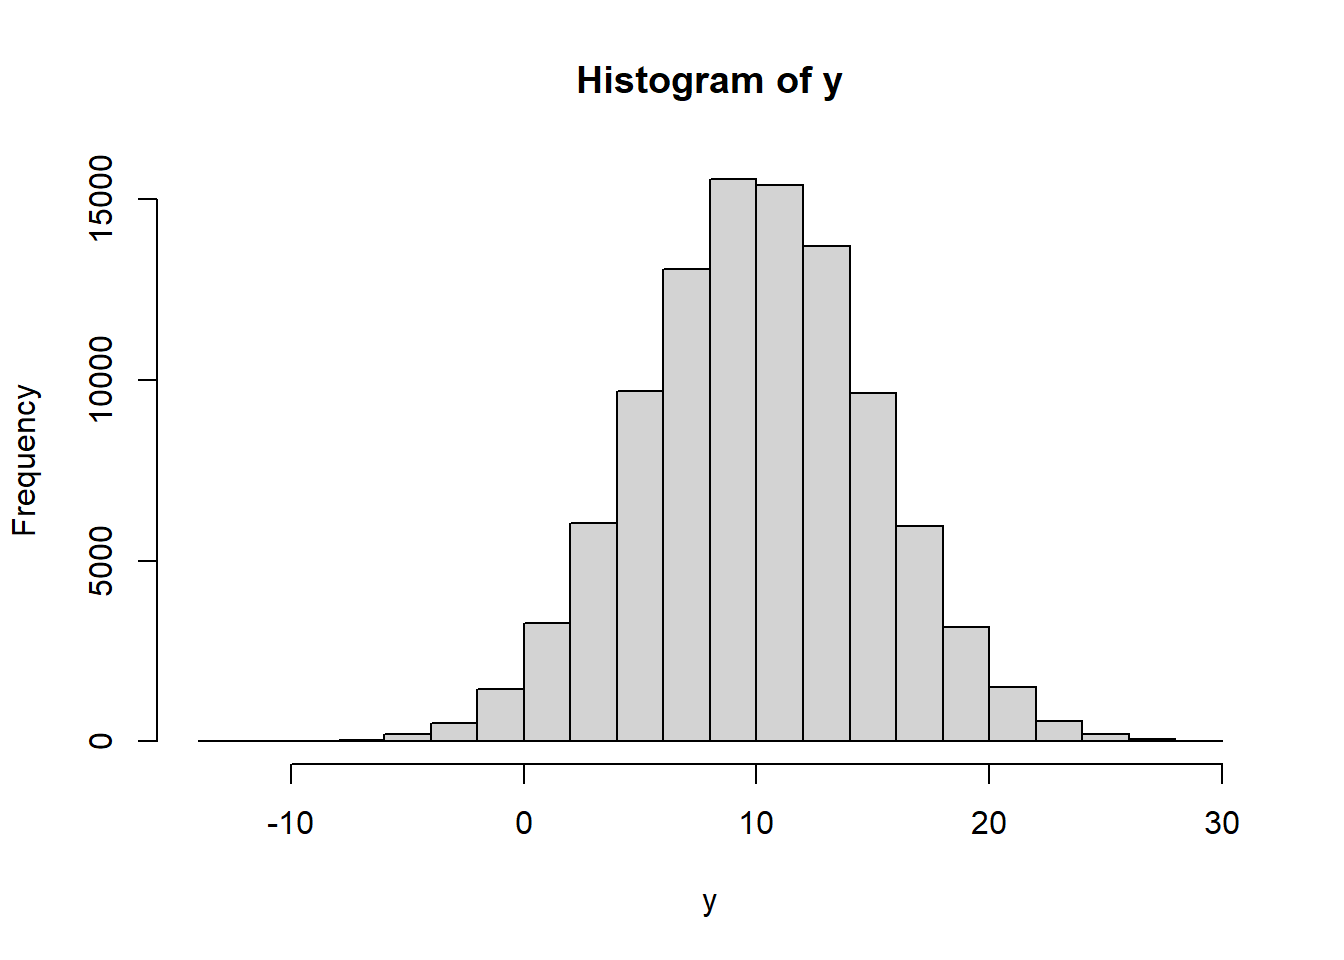
\includegraphics{bigdata_files/figure-latex/unnamed-chunk-21-1.pdf}

\begin{itemize}
\tightlist
\item
  Matrices
\end{itemize}

\begin{Shaded}
\begin{Highlighting}[]
\NormalTok{A<-}\KeywordTok{matrix}\NormalTok{(}\KeywordTok{c}\NormalTok{(}\DecValTok{1}\NormalTok{,}\DecValTok{2}\NormalTok{,}\DecValTok{3}\NormalTok{,}\DecValTok{4}\NormalTok{),}\DecValTok{2}\NormalTok{,}\DecValTok{2}\NormalTok{)}
\KeywordTok{matrix}\NormalTok{(}\KeywordTok{c}\NormalTok{(}\DecValTok{1}\NormalTok{,}\DecValTok{2}\NormalTok{,}\DecValTok{3}\NormalTok{,}\DecValTok{4}\NormalTok{),}\DecValTok{2}\NormalTok{,}\DecValTok{2}\NormalTok{,}\DataTypeTok{byrow=}\NormalTok{T)}
\end{Highlighting}
\end{Shaded}

\begin{verbatim}
##      [,1] [,2]
## [1,]    1    2
## [2,]    3    4
\end{verbatim}

\begin{Shaded}
\begin{Highlighting}[]
\NormalTok{B<-A}\OperatorTok{>=}\DecValTok{2}
\NormalTok{B}
\end{Highlighting}
\end{Shaded}

\begin{verbatim}
##       [,1] [,2]
## [1,] FALSE TRUE
## [2,]  TRUE TRUE
\end{verbatim}

\begin{Shaded}
\begin{Highlighting}[]
\KeywordTok{matrix}\NormalTok{(}\KeywordTok{c}\NormalTok{(}\StringTok{"Hola"}\NormalTok{,}\StringTok{"como"}\NormalTok{, }\StringTok{"estan"}\NormalTok{,}\StringTok{"chau"}\NormalTok{),}\DecValTok{2}\NormalTok{,}\DecValTok{2}\NormalTok{)}
\end{Highlighting}
\end{Shaded}

\begin{verbatim}
##      [,1]   [,2]   
## [1,] "Hola" "estan"
## [2,] "como" "chau"
\end{verbatim}

\begin{Shaded}
\begin{Highlighting}[]
\KeywordTok{matrix}\NormalTok{(}\KeywordTok{c}\NormalTok{(}\StringTok{"Hola"}\NormalTok{,}\DecValTok{1}\NormalTok{,}\DecValTok{2}\NormalTok{,}\DecValTok{3}\NormalTok{),}\DecValTok{2}\NormalTok{,}\DecValTok{2}\NormalTok{)}
\end{Highlighting}
\end{Shaded}

\begin{verbatim}
##      [,1]   [,2]
## [1,] "Hola" "2" 
## [2,] "1"    "3"
\end{verbatim}

\begin{Shaded}
\begin{Highlighting}[]
\KeywordTok{matrix}\NormalTok{(}\DecValTok{1}\OperatorTok{:}\DecValTok{10}\NormalTok{,}\DecValTok{2}\NormalTok{,}\DecValTok{5}\NormalTok{)}
\end{Highlighting}
\end{Shaded}

\begin{verbatim}
##      [,1] [,2] [,3] [,4] [,5]
## [1,]    1    3    5    7    9
## [2,]    2    4    6    8   10
\end{verbatim}

\begin{Shaded}
\begin{Highlighting}[]
\KeywordTok{matrix}\NormalTok{(}\DecValTok{1}\OperatorTok{:}\DecValTok{10}\NormalTok{,}\DecValTok{5}\NormalTok{,}\DecValTok{2}\NormalTok{)}
\end{Highlighting}
\end{Shaded}

\begin{verbatim}
##      [,1] [,2]
## [1,]    1    6
## [2,]    2    7
## [3,]    3    8
## [4,]    4    9
## [5,]    5   10
\end{verbatim}

\begin{Shaded}
\begin{Highlighting}[]
\KeywordTok{matrix}\NormalTok{(}\DecValTok{1}\OperatorTok{:}\DecValTok{10}\NormalTok{,}\DecValTok{5}\NormalTok{,}\DecValTok{5}\NormalTok{)}
\end{Highlighting}
\end{Shaded}

\begin{verbatim}
##      [,1] [,2] [,3] [,4] [,5]
## [1,]    1    6    1    6    1
## [2,]    2    7    2    7    2
## [3,]    3    8    3    8    3
## [4,]    4    9    4    9    4
## [5,]    5   10    5   10    5
\end{verbatim}

\begin{Shaded}
\begin{Highlighting}[]
\CommentTok{# funciones para crear otras matrices}
\KeywordTok{diag}\NormalTok{(}\DecValTok{1}\NormalTok{,}\DecValTok{5}\NormalTok{,}\DecValTok{5}\NormalTok{)}
\end{Highlighting}
\end{Shaded}

\begin{verbatim}
##      [,1] [,2] [,3] [,4] [,5]
## [1,]    1    0    0    0    0
## [2,]    0    1    0    0    0
## [3,]    0    0    1    0    0
## [4,]    0    0    0    1    0
## [5,]    0    0    0    0    1
\end{verbatim}

\begin{Shaded}
\begin{Highlighting}[]
\KeywordTok{diag}\NormalTok{(}\DecValTok{1}\OperatorTok{:}\DecValTok{5}\NormalTok{,}\DecValTok{5}\NormalTok{,}\DecValTok{5}\NormalTok{)}
\end{Highlighting}
\end{Shaded}

\begin{verbatim}
##      [,1] [,2] [,3] [,4] [,5]
## [1,]    1    0    0    0    0
## [2,]    0    2    0    0    0
## [3,]    0    0    3    0    0
## [4,]    0    0    0    4    0
## [5,]    0    0    0    0    5
\end{verbatim}

\begin{Shaded}
\begin{Highlighting}[]
\CommentTok{# Matriz inversa}
\NormalTok{C<-}\KeywordTok{matrix}\NormalTok{(}\KeywordTok{c}\NormalTok{(}\DecValTok{2}\NormalTok{,}\DecValTok{5}\NormalTok{,}\DecValTok{3}\NormalTok{,}\DecValTok{7}\NormalTok{),}\DecValTok{2}\NormalTok{,}\DecValTok{2}\NormalTok{)}
\KeywordTok{solve}\NormalTok{(C)}
\end{Highlighting}
\end{Shaded}

\begin{verbatim}
##      [,1] [,2]
## [1,]   -7    3
## [2,]    5   -2
\end{verbatim}

\begin{Shaded}
\begin{Highlighting}[]
\KeywordTok{det}\NormalTok{(C)}
\end{Highlighting}
\end{Shaded}

\begin{verbatim}
## [1] -1
\end{verbatim}

\begin{Shaded}
\begin{Highlighting}[]
\CommentTok{# operaciones con matrices}
\NormalTok{A}\OperatorTok{+}\NormalTok{C}
\end{Highlighting}
\end{Shaded}

\begin{verbatim}
##      [,1] [,2]
## [1,]    3    6
## [2,]    7   11
\end{verbatim}

\begin{Shaded}
\begin{Highlighting}[]
\NormalTok{A}\OperatorTok{-}\NormalTok{C}
\end{Highlighting}
\end{Shaded}

\begin{verbatim}
##      [,1] [,2]
## [1,]   -1    0
## [2,]   -3   -3
\end{verbatim}

\begin{Shaded}
\begin{Highlighting}[]
\NormalTok{A}\OperatorTok{*}\NormalTok{C }\CommentTok{# elemento a elemento}
\end{Highlighting}
\end{Shaded}

\begin{verbatim}
##      [,1] [,2]
## [1,]    2    9
## [2,]   10   28
\end{verbatim}

\begin{Shaded}
\begin{Highlighting}[]
\NormalTok{A }\OperatorTok\StringTok{ }\NormalTok{C }\CommentTok{# Multiplicación matricial}
\end{Highlighting}
\end{Shaded}

\begin{verbatim}
##      [,1] [,2]
## [1,]   17   24
## [2,]   24   34
\end{verbatim}

\begin{Shaded}
\begin{Highlighting}[]
\KeywordTok{t}\NormalTok{(C)}\CommentTok{# transpuesta}
\end{Highlighting}
\end{Shaded}

\begin{verbatim}
##      [,1] [,2]
## [1,]    2    5
## [2,]    3    7
\end{verbatim}

\begin{Shaded}
\begin{Highlighting}[]
\NormalTok{D<-C }\OperatorTok\StringTok{ }\KeywordTok{t}\NormalTok{(C)     }\CommentTok{# Simétrica}
\NormalTok{C }\OperatorTok\StringTok{ }\KeywordTok{solve}\NormalTok{(C) }\CommentTok{# Inversa}
\end{Highlighting}
\end{Shaded}

\begin{verbatim}
##      [,1]          [,2]
## [1,]    1 -8.881784e-16
## [2,]    0  1.000000e+00
\end{verbatim}

\begin{Shaded}
\begin{Highlighting}[]
\CommentTok{# Desc. Matriz}
\KeywordTok{eigen}\NormalTok{(D)}
\end{Highlighting}
\end{Shaded}

\begin{verbatim}
## eigen() decomposition
## $values
## [1] 86.98850423  0.01149577
## 
## $vectors
##           [,1]       [,2]
## [1,] 0.3864358 -0.9223163
## [2,] 0.9223163  0.3864358
\end{verbatim}

\begin{Shaded}
\begin{Highlighting}[]
\KeywordTok{svd}\NormalTok{(D)}
\end{Highlighting}
\end{Shaded}

\begin{verbatim}
## $d
## [1] 86.98850423  0.01149577
## 
## $u
##            [,1]       [,2]
## [1,] -0.3864358 -0.9223163
## [2,] -0.9223163  0.3864358
## 
## $v
##            [,1]       [,2]
## [1,] -0.3864358 -0.9223163
## [2,] -0.9223163  0.3864358
\end{verbatim}

\begin{Shaded}
\begin{Highlighting}[]
\KeywordTok{qr}\NormalTok{(D)}
\end{Highlighting}
\end{Shaded}

\begin{verbatim}
## $qr
##             [,1]         [,2]
## [1,] -33.6154726 -80.23091122
## [2,]   0.9221944   0.02974821
## 
## $rank
## [1] 2
## 
## $qraux
## [1] 1.38672668 0.02974821
## 
## $pivot
## [1] 1 2
## 
## attr(,"class")
## [1] "qr"
\end{verbatim}

\begin{Shaded}
\begin{Highlighting}[]
\KeywordTok{dim}\NormalTok{(D)}
\end{Highlighting}
\end{Shaded}

\begin{verbatim}
## [1] 2 2
\end{verbatim}

\begin{itemize}
\tightlist
\item
  Arrays (Generalización)
\end{itemize}

\begin{Shaded}
\begin{Highlighting}[]
\KeywordTok{array}\NormalTok{(}\DecValTok{1}\OperatorTok{:}\DecValTok{27}\NormalTok{,}\KeywordTok{c}\NormalTok{(}\DecValTok{3}\NormalTok{,}\DecValTok{3}\NormalTok{,}\DecValTok{3}\NormalTok{))}
\end{Highlighting}
\end{Shaded}

\begin{verbatim}
## , , 1
## 
##      [,1] [,2] [,3]
## [1,]    1    4    7
## [2,]    2    5    8
## [3,]    3    6    9
## 
## , , 2
## 
##      [,1] [,2] [,3]
## [1,]   10   13   16
## [2,]   11   14   17
## [3,]   12   15   18
## 
## , , 3
## 
##      [,1] [,2] [,3]
## [1,]   19   22   25
## [2,]   20   23   26
## [3,]   21   24   27
\end{verbatim}

\begin{Shaded}
\begin{Highlighting}[]
\KeywordTok{array}\NormalTok{(}\DecValTok{1}\OperatorTok{:}\DecValTok{81}\NormalTok{,}\KeywordTok{c}\NormalTok{(}\DecValTok{3}\NormalTok{,}\DecValTok{3}\NormalTok{,}\DecValTok{3}\NormalTok{,}\DecValTok{3}\NormalTok{))}
\end{Highlighting}
\end{Shaded}

\begin{verbatim}
## , , 1, 1
## 
##      [,1] [,2] [,3]
## [1,]    1    4    7
## [2,]    2    5    8
## [3,]    3    6    9
## 
## , , 2, 1
## 
##      [,1] [,2] [,3]
## [1,]   10   13   16
## [2,]   11   14   17
## [3,]   12   15   18
## 
## , , 3, 1
## 
##      [,1] [,2] [,3]
## [1,]   19   22   25
## [2,]   20   23   26
## [3,]   21   24   27
## 
## , , 1, 2
## 
##      [,1] [,2] [,3]
## [1,]   28   31   34
## [2,]   29   32   35
## [3,]   30   33   36
## 
## , , 2, 2
## 
##      [,1] [,2] [,3]
## [1,]   37   40   43
## [2,]   38   41   44
## [3,]   39   42   45
## 
## , , 3, 2
## 
##      [,1] [,2] [,3]
## [1,]   46   49   52
## [2,]   47   50   53
## [3,]   48   51   54
## 
## , , 1, 3
## 
##      [,1] [,2] [,3]
## [1,]   55   58   61
## [2,]   56   59   62
## [3,]   57   60   63
## 
## , , 2, 3
## 
##      [,1] [,2] [,3]
## [1,]   64   67   70
## [2,]   65   68   71
## [3,]   66   69   72
## 
## , , 3, 3
## 
##      [,1] [,2] [,3]
## [1,]   73   76   79
## [2,]   74   77   80
## [3,]   75   78   81
\end{verbatim}

\hypertarget{heteroguxe9neas}{%
\subsection{Heterogéneas}\label{heteroguxe9neas}}

Estas estructuras permiten el uso de diferentes tipos de clases u objetos.

\begin{itemize}
\tightlist
\item
  Dataframes (Bases de datos)
\end{itemize}

Tiene una estructura similar a una matriz, donde se define que las filas corresponden a observaciones/sujetos y las columnas son variables.

\begin{Shaded}
\begin{Highlighting}[]
\CommentTok{#encuesta en la sala de clases}
\NormalTok{id<-}\DecValTok{1}\OperatorTok{:}\DecValTok{8}
\NormalTok{name<-}\KeywordTok{c}\NormalTok{(}\StringTok{"adriana"}\NormalTok{,}\StringTok{"anahi"}\NormalTok{,}\StringTok{"miguel"}\NormalTok{,}\StringTok{"rayner"}\NormalTok{,}\StringTok{"rebeca"}\NormalTok{,}\StringTok{"sergio"}\NormalTok{,}\StringTok{"vania"}\NormalTok{,}\StringTok{"yoselin"}\NormalTok{)}
\NormalTok{mujer<-}\KeywordTok{c}\NormalTok{(}\DecValTok{1}\NormalTok{,}\DecValTok{1}\NormalTok{,}\DecValTok{0}\NormalTok{,}\DecValTok{0}\NormalTok{,}\DecValTok{1}\NormalTok{,}\DecValTok{0}\NormalTok{,}\DecValTok{1}\NormalTok{,}\DecValTok{1}\NormalTok{)}
\NormalTok{bd<-}\KeywordTok{data.frame}\NormalTok{(id,name,mujer)}
\NormalTok{bd}
\end{Highlighting}
\end{Shaded}

\begin{verbatim}
##   id    name mujer
## 1  1 adriana     1
## 2  2   anahi     1
## 3  3  miguel     0
## 4  4  rayner     0
## 5  5  rebeca     1
## 6  6  sergio     0
## 7  7   vania     1
## 8  8 yoselin     1
\end{verbatim}

\begin{Shaded}
\begin{Highlighting}[]
\KeywordTok{dim}\NormalTok{(bd)}
\end{Highlighting}
\end{Shaded}

\begin{verbatim}
## [1] 8 3
\end{verbatim}

\begin{Shaded}
\begin{Highlighting}[]
\KeywordTok{str}\NormalTok{(bd)}\CommentTok{# estructura del objeto}
\end{Highlighting}
\end{Shaded}

\begin{verbatim}
## 'data.frame':    8 obs. of  3 variables:
##  $ id   : int  1 2 3 4 5 6 7 8
##  $ name : chr  "adriana" "anahi" "miguel" "rayner" ...
##  $ mujer: num  1 1 0 0 1 0 1 1
\end{verbatim}

\begin{Shaded}
\begin{Highlighting}[]
\CommentTok{# incorporando variables}
\NormalTok{bd}\OperatorTok{$}\NormalTok{edad<-}\KeywordTok{round}\NormalTok{(}\KeywordTok{runif}\NormalTok{(}\DecValTok{8}\NormalTok{,}\DecValTok{19}\NormalTok{,}\DecValTok{25}\NormalTok{),}\DecValTok{0}\NormalTok{)}
\NormalTok{bd}
\end{Highlighting}
\end{Shaded}

\begin{verbatim}
##   id    name mujer edad
## 1  1 adriana     1   22
## 2  2   anahi     1   22
## 3  3  miguel     0   24
## 4  4  rayner     0   20
## 5  5  rebeca     1   23
## 6  6  sergio     0   21
## 7  7   vania     1   24
## 8  8 yoselin     1   21
\end{verbatim}

\begin{itemize}
\tightlist
\item
  Listas
  Las listas en R son de los objetos más poderosos que tiene, ya que permite almacenar todo.
\end{itemize}

\begin{Shaded}
\begin{Highlighting}[]
\NormalTok{w1<-}\KeywordTok{list}\NormalTok{(bd,bd,C,}\DecValTok{1}\OperatorTok{:}\DecValTok{10000}\NormalTok{,}\StringTok{"Hola"}\NormalTok{,}\DecValTok{1}\OperatorTok{:}\DecValTok{10}\OperatorTok{^}\DecValTok{6}\NormalTok{)}
\NormalTok{w1}
\end{Highlighting}
\end{Shaded}

\begin{verbatim}
## [[1]]
##   id    name mujer edad
## 1  1 adriana     1   22
## 2  2   anahi     1   22
## 3  3  miguel     0   24
## 4  4  rayner     0   20
## 5  5  rebeca     1   23
## 6  6  sergio     0   21
## 7  7   vania     1   24
## 8  8 yoselin     1   21
## 
## [[2]]
##   id    name mujer edad
## 1  1 adriana     1   22
## 2  2   anahi     1   22
## 3  3  miguel     0   24
## 4  4  rayner     0   20
## 5  5  rebeca     1   23
## 6  6  sergio     0   21
## 7  7   vania     1   24
## 8  8 yoselin     1   21
## 
## [[3]]
##      [,1] [,2]
## [1,]    2    3
## [2,]    5    7
## 
## [[4]]
##    [1]    1    2    3    4    5    6    7    8
##    [9]    9   10   11   12   13   14   15   16
##   [17]   17   18   19   20   21   22   23   24
##   [25]   25   26   27   28   29   30   31   32
##   [33]   33   34   35   36   37   38   39   40
##   [41]   41   42   43   44   45   46   47   48
##   [49]   49   50   51   52   53   54   55   56
##   [57]   57   58   59   60   61   62   63   64
##   [65]   65   66   67   68   69   70   71   72
##   [73]   73   74   75   76   77   78   79   80
##   [81]   81   82   83   84   85   86   87   88
##   [89]   89   90   91   92   93   94   95   96
##   [97]   97   98   99  100  101  102  103  104
##  [105]  105  106  107  108  109  110  111  112
##  [113]  113  114  115  116  117  118  119  120
##  [121]  121  122  123  124  125  126  127  128
##  [129]  129  130  131  132  133  134  135  136
##  [137]  137  138  139  140  141  142  143  144
##  [145]  145  146  147  148  149  150  151  152
##  [153]  153  154  155  156  157  158  159  160
##  [161]  161  162  163  164  165  166  167  168
##  [169]  169  170  171  172  173  174  175  176
##  [177]  177  178  179  180  181  182  183  184
##  [185]  185  186  187  188  189  190  191  192
##  [193]  193  194  195  196  197  198  199  200
##  [201]  201  202  203  204  205  206  207  208
##  [209]  209  210  211  212  213  214  215  216
##  [217]  217  218  219  220  221  222  223  224
##  [225]  225  226  227  228  229  230  231  232
##  [233]  233  234  235  236  237  238  239  240
##  [241]  241  242  243  244  245  246  247  248
##  [249]  249  250  251  252  253  254  255  256
##  [257]  257  258  259  260  261  262  263  264
##  [265]  265  266  267  268  269  270  271  272
##  [273]  273  274  275  276  277  278  279  280
##  [281]  281  282  283  284  285  286  287  288
##  [289]  289  290  291  292  293  294  295  296
##  [297]  297  298  299  300  301  302  303  304
##  [305]  305  306  307  308  309  310  311  312
##  [313]  313  314  315  316  317  318  319  320
##  [321]  321  322  323  324  325  326  327  328
##  [329]  329  330  331  332  333  334  335  336
##  [337]  337  338  339  340  341  342  343  344
##  [345]  345  346  347  348  349  350  351  352
##  [353]  353  354  355  356  357  358  359  360
##  [361]  361  362  363  364  365  366  367  368
##  [369]  369  370  371  372  373  374  375  376
##  [377]  377  378  379  380  381  382  383  384
##  [385]  385  386  387  388  389  390  391  392
##  [393]  393  394  395  396  397  398  399  400
##  [401]  401  402  403  404  405  406  407  408
##  [409]  409  410  411  412  413  414  415  416
##  [417]  417  418  419  420  421  422  423  424
##  [425]  425  426  427  428  429  430  431  432
##  [433]  433  434  435  436  437  438  439  440
##  [441]  441  442  443  444  445  446  447  448
##  [449]  449  450  451  452  453  454  455  456
##  [457]  457  458  459  460  461  462  463  464
##  [465]  465  466  467  468  469  470  471  472
##  [473]  473  474  475  476  477  478  479  480
##  [481]  481  482  483  484  485  486  487  488
##  [489]  489  490  491  492  493  494  495  496
##  [497]  497  498  499  500  501  502  503  504
##  [505]  505  506  507  508  509  510  511  512
##  [513]  513  514  515  516  517  518  519  520
##  [521]  521  522  523  524  525  526  527  528
##  [529]  529  530  531  532  533  534  535  536
##  [537]  537  538  539  540  541  542  543  544
##  [545]  545  546  547  548  549  550  551  552
##  [553]  553  554  555  556  557  558  559  560
##  [561]  561  562  563  564  565  566  567  568
##  [569]  569  570  571  572  573  574  575  576
##  [577]  577  578  579  580  581  582  583  584
##  [585]  585  586  587  588  589  590  591  592
##  [593]  593  594  595  596  597  598  599  600
##  [601]  601  602  603  604  605  606  607  608
##  [609]  609  610  611  612  613  614  615  616
##  [617]  617  618  619  620  621  622  623  624
##  [625]  625  626  627  628  629  630  631  632
##  [633]  633  634  635  636  637  638  639  640
##  [641]  641  642  643  644  645  646  647  648
##  [649]  649  650  651  652  653  654  655  656
##  [657]  657  658  659  660  661  662  663  664
##  [665]  665  666  667  668  669  670  671  672
##  [673]  673  674  675  676  677  678  679  680
##  [681]  681  682  683  684  685  686  687  688
##  [689]  689  690  691  692  693  694  695  696
##  [697]  697  698  699  700  701  702  703  704
##  [705]  705  706  707  708  709  710  711  712
##  [713]  713  714  715  716  717  718  719  720
##  [721]  721  722  723  724  725  726  727  728
##  [729]  729  730  731  732  733  734  735  736
##  [737]  737  738  739  740  741  742  743  744
##  [745]  745  746  747  748  749  750  751  752
##  [753]  753  754  755  756  757  758  759  760
##  [761]  761  762  763  764  765  766  767  768
##  [769]  769  770  771  772  773  774  775  776
##  [777]  777  778  779  780  781  782  783  784
##  [785]  785  786  787  788  789  790  791  792
##  [793]  793  794  795  796  797  798  799  800
##  [801]  801  802  803  804  805  806  807  808
##  [809]  809  810  811  812  813  814  815  816
##  [817]  817  818  819  820  821  822  823  824
##  [825]  825  826  827  828  829  830  831  832
##  [833]  833  834  835  836  837  838  839  840
##  [841]  841  842  843  844  845  846  847  848
##  [849]  849  850  851  852  853  854  855  856
##  [857]  857  858  859  860  861  862  863  864
##  [865]  865  866  867  868  869  870  871  872
##  [873]  873  874  875  876  877  878  879  880
##  [881]  881  882  883  884  885  886  887  888
##  [889]  889  890  891  892  893  894  895  896
##  [897]  897  898  899  900  901  902  903  904
##  [905]  905  906  907  908  909  910  911  912
##  [913]  913  914  915  916  917  918  919  920
##  [921]  921  922  923  924  925  926  927  928
##  [929]  929  930  931  932  933  934  935  936
##  [937]  937  938  939  940  941  942  943  944
##  [945]  945  946  947  948  949  950  951  952
##  [953]  953  954  955  956  957  958  959  960
##  [961]  961  962  963  964  965  966  967  968
##  [969]  969  970  971  972  973  974  975  976
##  [977]  977  978  979  980  981  982  983  984
##  [985]  985  986  987  988  989  990  991  992
##  [993]  993  994  995  996  997  998  999 1000
##  [ reached getOption("max.print") -- omitted 9000 entries ]
## 
## [[5]]
## [1] "Hola"
## 
## [[6]]
##    [1]    1    2    3    4    5    6    7    8
##    [9]    9   10   11   12   13   14   15   16
##   [17]   17   18   19   20   21   22   23   24
##   [25]   25   26   27   28   29   30   31   32
##   [33]   33   34   35   36   37   38   39   40
##   [41]   41   42   43   44   45   46   47   48
##   [49]   49   50   51   52   53   54   55   56
##   [57]   57   58   59   60   61   62   63   64
##   [65]   65   66   67   68   69   70   71   72
##   [73]   73   74   75   76   77   78   79   80
##   [81]   81   82   83   84   85   86   87   88
##   [89]   89   90   91   92   93   94   95   96
##   [97]   97   98   99  100  101  102  103  104
##  [105]  105  106  107  108  109  110  111  112
##  [113]  113  114  115  116  117  118  119  120
##  [121]  121  122  123  124  125  126  127  128
##  [129]  129  130  131  132  133  134  135  136
##  [137]  137  138  139  140  141  142  143  144
##  [145]  145  146  147  148  149  150  151  152
##  [153]  153  154  155  156  157  158  159  160
##  [161]  161  162  163  164  165  166  167  168
##  [169]  169  170  171  172  173  174  175  176
##  [177]  177  178  179  180  181  182  183  184
##  [185]  185  186  187  188  189  190  191  192
##  [193]  193  194  195  196  197  198  199  200
##  [201]  201  202  203  204  205  206  207  208
##  [209]  209  210  211  212  213  214  215  216
##  [217]  217  218  219  220  221  222  223  224
##  [225]  225  226  227  228  229  230  231  232
##  [233]  233  234  235  236  237  238  239  240
##  [241]  241  242  243  244  245  246  247  248
##  [249]  249  250  251  252  253  254  255  256
##  [257]  257  258  259  260  261  262  263  264
##  [265]  265  266  267  268  269  270  271  272
##  [273]  273  274  275  276  277  278  279  280
##  [281]  281  282  283  284  285  286  287  288
##  [289]  289  290  291  292  293  294  295  296
##  [297]  297  298  299  300  301  302  303  304
##  [305]  305  306  307  308  309  310  311  312
##  [313]  313  314  315  316  317  318  319  320
##  [321]  321  322  323  324  325  326  327  328
##  [329]  329  330  331  332  333  334  335  336
##  [337]  337  338  339  340  341  342  343  344
##  [345]  345  346  347  348  349  350  351  352
##  [353]  353  354  355  356  357  358  359  360
##  [361]  361  362  363  364  365  366  367  368
##  [369]  369  370  371  372  373  374  375  376
##  [377]  377  378  379  380  381  382  383  384
##  [385]  385  386  387  388  389  390  391  392
##  [393]  393  394  395  396  397  398  399  400
##  [401]  401  402  403  404  405  406  407  408
##  [409]  409  410  411  412  413  414  415  416
##  [417]  417  418  419  420  421  422  423  424
##  [425]  425  426  427  428  429  430  431  432
##  [433]  433  434  435  436  437  438  439  440
##  [441]  441  442  443  444  445  446  447  448
##  [449]  449  450  451  452  453  454  455  456
##  [457]  457  458  459  460  461  462  463  464
##  [465]  465  466  467  468  469  470  471  472
##  [473]  473  474  475  476  477  478  479  480
##  [481]  481  482  483  484  485  486  487  488
##  [489]  489  490  491  492  493  494  495  496
##  [497]  497  498  499  500  501  502  503  504
##  [505]  505  506  507  508  509  510  511  512
##  [513]  513  514  515  516  517  518  519  520
##  [521]  521  522  523  524  525  526  527  528
##  [529]  529  530  531  532  533  534  535  536
##  [537]  537  538  539  540  541  542  543  544
##  [545]  545  546  547  548  549  550  551  552
##  [553]  553  554  555  556  557  558  559  560
##  [561]  561  562  563  564  565  566  567  568
##  [569]  569  570  571  572  573  574  575  576
##  [577]  577  578  579  580  581  582  583  584
##  [585]  585  586  587  588  589  590  591  592
##  [593]  593  594  595  596  597  598  599  600
##  [601]  601  602  603  604  605  606  607  608
##  [609]  609  610  611  612  613  614  615  616
##  [617]  617  618  619  620  621  622  623  624
##  [625]  625  626  627  628  629  630  631  632
##  [633]  633  634  635  636  637  638  639  640
##  [641]  641  642  643  644  645  646  647  648
##  [649]  649  650  651  652  653  654  655  656
##  [657]  657  658  659  660  661  662  663  664
##  [665]  665  666  667  668  669  670  671  672
##  [673]  673  674  675  676  677  678  679  680
##  [681]  681  682  683  684  685  686  687  688
##  [689]  689  690  691  692  693  694  695  696
##  [697]  697  698  699  700  701  702  703  704
##  [705]  705  706  707  708  709  710  711  712
##  [713]  713  714  715  716  717  718  719  720
##  [721]  721  722  723  724  725  726  727  728
##  [729]  729  730  731  732  733  734  735  736
##  [737]  737  738  739  740  741  742  743  744
##  [745]  745  746  747  748  749  750  751  752
##  [753]  753  754  755  756  757  758  759  760
##  [761]  761  762  763  764  765  766  767  768
##  [769]  769  770  771  772  773  774  775  776
##  [777]  777  778  779  780  781  782  783  784
##  [785]  785  786  787  788  789  790  791  792
##  [793]  793  794  795  796  797  798  799  800
##  [801]  801  802  803  804  805  806  807  808
##  [809]  809  810  811  812  813  814  815  816
##  [817]  817  818  819  820  821  822  823  824
##  [825]  825  826  827  828  829  830  831  832
##  [833]  833  834  835  836  837  838  839  840
##  [841]  841  842  843  844  845  846  847  848
##  [849]  849  850  851  852  853  854  855  856
##  [857]  857  858  859  860  861  862  863  864
##  [865]  865  866  867  868  869  870  871  872
##  [873]  873  874  875  876  877  878  879  880
##  [881]  881  882  883  884  885  886  887  888
##  [889]  889  890  891  892  893  894  895  896
##  [897]  897  898  899  900  901  902  903  904
##  [905]  905  906  907  908  909  910  911  912
##  [913]  913  914  915  916  917  918  919  920
##  [921]  921  922  923  924  925  926  927  928
##  [929]  929  930  931  932  933  934  935  936
##  [937]  937  938  939  940  941  942  943  944
##  [945]  945  946  947  948  949  950  951  952
##  [953]  953  954  955  956  957  958  959  960
##  [961]  961  962  963  964  965  966  967  968
##  [969]  969  970  971  972  973  974  975  976
##  [977]  977  978  979  980  981  982  983  984
##  [985]  985  986  987  988  989  990  991  992
##  [993]  993  994  995  996  997  998  999 1000
##  [ reached getOption("max.print") -- omitted 999000 entries ]
\end{verbatim}

\begin{Shaded}
\begin{Highlighting}[]
\KeywordTok{str}\NormalTok{(w1)}
\end{Highlighting}
\end{Shaded}

\begin{verbatim}
## List of 6
##  $ :'data.frame':    8 obs. of  4 variables:
##   ..$ id   : int [1:8] 1 2 3 4 5 6 7 8
##   ..$ name : chr [1:8] "adriana" "anahi" "miguel" "rayner" ...
##   ..$ mujer: num [1:8] 1 1 0 0 1 0 1 1
##   ..$ edad : num [1:8] 22 22 24 20 23 21 24 21
##  $ :'data.frame':    8 obs. of  4 variables:
##   ..$ id   : int [1:8] 1 2 3 4 5 6 7 8
##   ..$ name : chr [1:8] "adriana" "anahi" "miguel" "rayner" ...
##   ..$ mujer: num [1:8] 1 1 0 0 1 0 1 1
##   ..$ edad : num [1:8] 22 22 24 20 23 21 24 21
##  $ : num [1:2, 1:2] 2 5 3 7
##  $ : int [1:10000] 1 2 3 4 5 6 7 8 9 10 ...
##  $ : chr "Hola"
##  $ : int [1:1000000] 1 2 3 4 5 6 7 8 9 10 ...
\end{verbatim}

\begin{Shaded}
\begin{Highlighting}[]
\KeywordTok{object.size}\NormalTok{(w1)}\OperatorTok{/}\DecValTok{10}\OperatorTok{^}\DecValTok{6}
\end{Highlighting}
\end{Shaded}

\begin{verbatim}
## 4 bytes
\end{verbatim}

\begin{Shaded}
\begin{Highlighting}[]
\NormalTok{w2<-}\KeywordTok{list}\NormalTok{(w1,w1,}\KeywordTok{list}\NormalTok{(w1,C),C,}\DecValTok{1}\OperatorTok{:}\DecValTok{1000}\NormalTok{) }\CommentTok{# R puede encapsular objetos de tipo}
\KeywordTok{str}\NormalTok{(w2)}
\end{Highlighting}
\end{Shaded}

\begin{verbatim}
## List of 5
##  $ :List of 6
##   ..$ :'data.frame': 8 obs. of  4 variables:
##   .. ..$ id   : int [1:8] 1 2 3 4 5 6 7 8
##   .. ..$ name : chr [1:8] "adriana" "anahi" "miguel" "rayner" ...
##   .. ..$ mujer: num [1:8] 1 1 0 0 1 0 1 1
##   .. ..$ edad : num [1:8] 22 22 24 20 23 21 24 21
##   ..$ :'data.frame': 8 obs. of  4 variables:
##   .. ..$ id   : int [1:8] 1 2 3 4 5 6 7 8
##   .. ..$ name : chr [1:8] "adriana" "anahi" "miguel" "rayner" ...
##   .. ..$ mujer: num [1:8] 1 1 0 0 1 0 1 1
##   .. ..$ edad : num [1:8] 22 22 24 20 23 21 24 21
##   ..$ : num [1:2, 1:2] 2 5 3 7
##   ..$ : int [1:10000] 1 2 3 4 5 6 7 8 9 10 ...
##   ..$ : chr "Hola"
##   ..$ : int [1:1000000] 1 2 3 4 5 6 7 8 9 10 ...
##  $ :List of 6
##   ..$ :'data.frame': 8 obs. of  4 variables:
##   .. ..$ id   : int [1:8] 1 2 3 4 5 6 7 8
##   .. ..$ name : chr [1:8] "adriana" "anahi" "miguel" "rayner" ...
##   .. ..$ mujer: num [1:8] 1 1 0 0 1 0 1 1
##   .. ..$ edad : num [1:8] 22 22 24 20 23 21 24 21
##   ..$ :'data.frame': 8 obs. of  4 variables:
##   .. ..$ id   : int [1:8] 1 2 3 4 5 6 7 8
##   .. ..$ name : chr [1:8] "adriana" "anahi" "miguel" "rayner" ...
##   .. ..$ mujer: num [1:8] 1 1 0 0 1 0 1 1
##   .. ..$ edad : num [1:8] 22 22 24 20 23 21 24 21
##   ..$ : num [1:2, 1:2] 2 5 3 7
##   ..$ : int [1:10000] 1 2 3 4 5 6 7 8 9 10 ...
##   ..$ : chr "Hola"
##   ..$ : int [1:1000000] 1 2 3 4 5 6 7 8 9 10 ...
##  $ :List of 2
##   ..$ :List of 6
##   .. ..$ :'data.frame':  8 obs. of  4 variables:
##   .. .. ..$ id   : int [1:8] 1 2 3 4 5 6 7 8
##   .. .. ..$ name : chr [1:8] "adriana" "anahi" "miguel" "rayner" ...
##   .. .. ..$ mujer: num [1:8] 1 1 0 0 1 0 1 1
##   .. .. ..$ edad : num [1:8] 22 22 24 20 23 21 24 21
##   .. ..$ :'data.frame':  8 obs. of  4 variables:
##   .. .. ..$ id   : int [1:8] 1 2 3 4 5 6 7 8
##   .. .. ..$ name : chr [1:8] "adriana" "anahi" "miguel" "rayner" ...
##   .. .. ..$ mujer: num [1:8] 1 1 0 0 1 0 1 1
##   .. .. ..$ edad : num [1:8] 22 22 24 20 23 21 24 21
##   .. ..$ : num [1:2, 1:2] 2 5 3 7
##   .. ..$ : int [1:10000] 1 2 3 4 5 6 7 8 9 10 ...
##   .. ..$ : chr "Hola"
##   .. ..$ : int [1:1000000] 1 2 3 4 5 6 7 8 9 10 ...
##   ..$ : num [1:2, 1:2] 2 5 3 7
##  $ : num [1:2, 1:2] 2 5 3 7
##  $ : int [1:1000] 1 2 3 4 5 6 7 8 9 10 ...
\end{verbatim}

\begin{Shaded}
\begin{Highlighting}[]
\KeywordTok{object.size}\NormalTok{(w2)}\OperatorTok{/}\DecValTok{10}\OperatorTok{^}\DecValTok{6}
\end{Highlighting}
\end{Shaded}

\begin{verbatim}
## 12.1 bytes
\end{verbatim}

\hypertarget{indexaciuxf3n}{%
\section{Indexación}\label{indexaciuxf3n}}

Es el proceso de manejar los elementos dentro de los objetos.

\begin{Shaded}
\begin{Highlighting}[]
\CommentTok{#VECTORES}
\NormalTok{x<-}\DecValTok{1}\OperatorTok{:}\DecValTok{100}
\NormalTok{x[}\KeywordTok{c}\NormalTok{(}\DecValTok{1}\NormalTok{,}\DecValTok{5}\NormalTok{,}\DecValTok{7}\NormalTok{)]}
\end{Highlighting}
\end{Shaded}

\begin{verbatim}
## [1] 1 5 7
\end{verbatim}

\begin{Shaded}
\begin{Highlighting}[]
\NormalTok{x[}\OperatorTok{-}\KeywordTok{c}\NormalTok{(}\DecValTok{1}\NormalTok{,}\DecValTok{5}\NormalTok{,}\DecValTok{7}\NormalTok{)]}
\end{Highlighting}
\end{Shaded}

\begin{verbatim}
##  [1]   2   3   4   6   8   9  10  11  12  13
## [11]  14  15  16  17  18  19  20  21  22  23
## [21]  24  25  26  27  28  29  30  31  32  33
## [31]  34  35  36  37  38  39  40  41  42  43
## [41]  44  45  46  47  48  49  50  51  52  53
## [51]  54  55  56  57  58  59  60  61  62  63
## [61]  64  65  66  67  68  69  70  71  72  73
## [71]  74  75  76  77  78  79  80  81  82  83
## [81]  84  85  86  87  88  89  90  91  92  93
## [91]  94  95  96  97  98  99 100
\end{verbatim}

\begin{Shaded}
\begin{Highlighting}[]
\NormalTok{o<-(x }\OperatorTok\StringTok{ }\DecValTok{2}\NormalTok{)}\OperatorTok{==}\DecValTok{0}
\NormalTok{x[o]}
\end{Highlighting}
\end{Shaded}

\begin{verbatim}
##  [1]   2   4   6   8  10  12  14  16  18  20
## [11]  22  24  26  28  30  32  34  36  38  40
## [21]  42  44  46  48  50  52  54  56  58  60
## [31]  62  64  66  68  70  72  74  76  78  80
## [41]  82  84  86  88  90  92  94  96  98 100
\end{verbatim}

\begin{Shaded}
\begin{Highlighting}[]
\NormalTok{x2<-}\KeywordTok{c}\NormalTok{(}\DecValTok{2}\NormalTok{,}\DecValTok{3}\NormalTok{,}\DecValTok{7}\NormalTok{,}\DecValTok{4}\NormalTok{)}
\NormalTok{x2[}\KeywordTok{c}\NormalTok{(T,T,F,F)]}
\end{Highlighting}
\end{Shaded}

\begin{verbatim}
## [1] 2 3
\end{verbatim}

\begin{Shaded}
\begin{Highlighting}[]
\CommentTok{#matrices}
\NormalTok{A<-}\KeywordTok{matrix}\NormalTok{(}\DecValTok{1}\OperatorTok{:}\DecValTok{30}\NormalTok{,}\DecValTok{5}\NormalTok{,}\DecValTok{6}\NormalTok{)}
\NormalTok{A[ }\DecValTok{3}\NormalTok{, }\DecValTok{4}\NormalTok{]}
\end{Highlighting}
\end{Shaded}

\begin{verbatim}
## [1] 18
\end{verbatim}

\begin{Shaded}
\begin{Highlighting}[]
\NormalTok{A[}\DecValTok{3}\NormalTok{, ]}
\end{Highlighting}
\end{Shaded}

\begin{verbatim}
## [1]  3  8 13 18 23 28
\end{verbatim}

\begin{Shaded}
\begin{Highlighting}[]
\NormalTok{A[}\KeywordTok{c}\NormalTok{(}\DecValTok{1}\NormalTok{,}\DecValTok{4}\NormalTok{), ]}
\end{Highlighting}
\end{Shaded}

\begin{verbatim}
##      [,1] [,2] [,3] [,4] [,5] [,6]
## [1,]    1    6   11   16   21   26
## [2,]    4    9   14   19   24   29
\end{verbatim}

\begin{Shaded}
\begin{Highlighting}[]
\NormalTok{A[,}\DecValTok{1}\OperatorTok{:}\DecValTok{2}\NormalTok{ ]}
\end{Highlighting}
\end{Shaded}

\begin{verbatim}
##      [,1] [,2]
## [1,]    1    6
## [2,]    2    7
## [3,]    3    8
## [4,]    4    9
## [5,]    5   10
\end{verbatim}

\begin{Shaded}
\begin{Highlighting}[]
\NormalTok{A[,}\OperatorTok{-}\KeywordTok{c}\NormalTok{(}\DecValTok{1}\OperatorTok{:}\DecValTok{2}\NormalTok{) ]}
\end{Highlighting}
\end{Shaded}

\begin{verbatim}
##      [,1] [,2] [,3] [,4]
## [1,]   11   16   21   26
## [2,]   12   17   22   27
## [3,]   13   18   23   28
## [4,]   14   19   24   29
## [5,]   15   20   25   30
\end{verbatim}

\begin{Shaded}
\begin{Highlighting}[]
\NormalTok{A[}\DecValTok{3}\OperatorTok{:}\DecValTok{4}\NormalTok{,}\KeywordTok{c}\NormalTok{(}\DecValTok{1}\NormalTok{,}\DecValTok{3}\NormalTok{)]}
\end{Highlighting}
\end{Shaded}

\begin{verbatim}
##      [,1] [,2]
## [1,]    3   13
## [2,]    4   14
\end{verbatim}

\begin{Shaded}
\begin{Highlighting}[]
\NormalTok{A[}\KeywordTok{c}\NormalTok{(T,T,F,T,T),}\KeywordTok{c}\NormalTok{(T,F,T,T,T,F)]}
\end{Highlighting}
\end{Shaded}

\begin{verbatim}
##      [,1] [,2] [,3] [,4]
## [1,]    1   11   16   21
## [2,]    2   12   17   22
## [3,]    4   14   19   24
## [4,]    5   15   20   25
\end{verbatim}

\begin{Shaded}
\begin{Highlighting}[]
\CommentTok{#data frame}
\NormalTok{bd[}\DecValTok{1}\OperatorTok{:}\DecValTok{3}\NormalTok{,}\DecValTok{2}\OperatorTok{:}\DecValTok{3}\NormalTok{]}
\end{Highlighting}
\end{Shaded}

\begin{verbatim}
##      name mujer
## 1 adriana     1
## 2   anahi     1
## 3  miguel     0
\end{verbatim}

\begin{Shaded}
\begin{Highlighting}[]
\CommentTok{# también es posible usar el nombre de las variables }
\NormalTok{bd[}\DecValTok{1}\OperatorTok{:}\DecValTok{6}\NormalTok{,}\KeywordTok{c}\NormalTok{(}\StringTok{"name"}\NormalTok{,}\StringTok{"id"}\NormalTok{)]}
\end{Highlighting}
\end{Shaded}

\begin{verbatim}
##      name id
## 1 adriana  1
## 2   anahi  2
## 3  miguel  3
## 4  rayner  4
## 5  rebeca  5
## 6  sergio  6
\end{verbatim}

\begin{Shaded}
\begin{Highlighting}[]
\NormalTok{bd[,}\OperatorTok{-}\KeywordTok{c}\NormalTok{(}\DecValTok{3}\NormalTok{)]}
\end{Highlighting}
\end{Shaded}

\begin{verbatim}
##   id    name edad
## 1  1 adriana   22
## 2  2   anahi   22
## 3  3  miguel   24
## 4  4  rayner   20
## 5  5  rebeca   23
## 6  6  sergio   21
## 7  7   vania   24
## 8  8 yoselin   21
\end{verbatim}

\begin{Shaded}
\begin{Highlighting}[]
\NormalTok{bd}\OperatorTok{$}\NormalTok{mujer}
\end{Highlighting}
\end{Shaded}

\begin{verbatim}
## [1] 1 1 0 0 1 0 1 1
\end{verbatim}

\begin{Shaded}
\begin{Highlighting}[]
\KeywordTok{mean}\NormalTok{(bd}\OperatorTok{$}\NormalTok{mujer)}
\end{Highlighting}
\end{Shaded}

\begin{verbatim}
## [1] 0.625
\end{verbatim}

\begin{Shaded}
\begin{Highlighting}[]
\NormalTok{bd[}\KeywordTok{c}\NormalTok{(}\DecValTok{2}\NormalTok{,}\DecValTok{6}\NormalTok{,}\DecValTok{8}\NormalTok{),]}
\end{Highlighting}
\end{Shaded}

\begin{verbatim}
##   id    name mujer edad
## 2  2   anahi     1   22
## 6  6  sergio     0   21
## 8  8 yoselin     1   21
\end{verbatim}

\begin{Shaded}
\begin{Highlighting}[]
\NormalTok{bd[bd}\OperatorTok{$}\NormalTok{edad}\OperatorTok{<=}\DecValTok{21} \OperatorTok{&}\StringTok{ }\NormalTok{bd}\OperatorTok{$}\NormalTok{mujer}\OperatorTok{==}\DecValTok{1}\NormalTok{,]}
\end{Highlighting}
\end{Shaded}

\begin{verbatim}
##   id    name mujer edad
## 8  8 yoselin     1   21
\end{verbatim}

\begin{Shaded}
\begin{Highlighting}[]
\CommentTok{#bd %>% filter(mujer==1 & edad<=21)}
\end{Highlighting}
\end{Shaded}

\hypertarget{loops-y-condiciones}{%
\section{Loops y condiciones}\label{loops-y-condiciones}}

\begin{Shaded}
\begin{Highlighting}[]
\KeywordTok{rm}\NormalTok{(}\DataTypeTok{list =} \KeywordTok{ls}\NormalTok{())}
\NormalTok{x<-}\DecValTok{5}
\CommentTok{## if}
\ControlFlowTok{if}\NormalTok{(x}\OperatorTok{>}\DecValTok{6}\NormalTok{)\{}
  \KeywordTok{hist}\NormalTok{(}\KeywordTok{rnorm}\NormalTok{(}\DecValTok{100}\NormalTok{,}\DecValTok{3}\NormalTok{,}\DecValTok{2}\NormalTok{))}
\NormalTok{\}}
\CommentTok{## if else}
\ControlFlowTok{if}\NormalTok{(x}\OperatorTok{>}\DecValTok{6}\NormalTok{)\{}
  \KeywordTok{hist}\NormalTok{(}\KeywordTok{rnorm}\NormalTok{(}\DecValTok{100}\NormalTok{,}\DecValTok{3}\NormalTok{,}\DecValTok{2}\NormalTok{))}
\NormalTok{\} }\ControlFlowTok{else}\NormalTok{ \{}
  \KeywordTok{boxplot}\NormalTok{(}\KeywordTok{rnorm}\NormalTok{(}\DecValTok{100}\NormalTok{,}\DecValTok{3}\NormalTok{,}\DecValTok{2}\NormalTok{))}
\NormalTok{\}}
\CommentTok{## if encadenado}
\NormalTok{x<-}\DecValTok{60}
\ControlFlowTok{if}\NormalTok{(x}\OperatorTok{>}\DecValTok{6}\NormalTok{)\{}
  \KeywordTok{hist}\NormalTok{(}\KeywordTok{rnorm}\NormalTok{(}\DecValTok{100}\NormalTok{,}\DecValTok{3}\NormalTok{,}\DecValTok{2}\NormalTok{))}
  \KeywordTok{mean}\NormalTok{(x)}
\NormalTok{\} }\ControlFlowTok{else} \ControlFlowTok{if}\NormalTok{(x}\OperatorTok{<}\DecValTok{6}\NormalTok{)\{}
  \KeywordTok{boxplot}\NormalTok{(}\KeywordTok{rnorm}\NormalTok{(}\DecValTok{100}\NormalTok{,}\DecValTok{3}\NormalTok{,}\DecValTok{2}\NormalTok{))}
\NormalTok{\} }\ControlFlowTok{else} \ControlFlowTok{if}\NormalTok{(}\KeywordTok{typeof}\NormalTok{(x)}\OperatorTok{==}\StringTok{"double"}\NormalTok{)\{}
  \KeywordTok{print}\NormalTok{(}\StringTok{"hola"}\NormalTok{)}
\NormalTok{\} }\ControlFlowTok{else}\NormalTok{ \{}
  \KeywordTok{print}\NormalTok{(}\StringTok{"hola hola"}\NormalTok{)}
\NormalTok{\}}
\CommentTok{##for}
\ControlFlowTok{for}\NormalTok{(i }\ControlFlowTok{in} \DecValTok{1}\OperatorTok{:}\DecValTok{100}\NormalTok{)\{}
  \KeywordTok{print}\NormalTok{(i)}
\NormalTok{\}}
\ControlFlowTok{for}\NormalTok{(i }\ControlFlowTok{in} \KeywordTok{c}\NormalTok{(}\DecValTok{2}\NormalTok{,}\DecValTok{7}\NormalTok{,}\DecValTok{9}\NormalTok{,}\DecValTok{15}\NormalTok{,}\DecValTok{19}\NormalTok{))\{}
  \KeywordTok{print}\NormalTok{(i)}
\NormalTok{\}  }
\ControlFlowTok{for}\NormalTok{(i }\ControlFlowTok{in} \KeywordTok{c}\NormalTok{(}\StringTok{"a"}\NormalTok{,}\StringTok{"b"}\NormalTok{,}\StringTok{"c"}\NormalTok{))\{}
  \KeywordTok{print}\NormalTok{(i)}
\NormalTok{\}  }
\ControlFlowTok{for}\NormalTok{(i }\ControlFlowTok{in} \DecValTok{1}\OperatorTok{:}\DecValTok{5}\NormalTok{)\{}
  \ControlFlowTok{for}\NormalTok{(j }\ControlFlowTok{in} \DecValTok{6}\OperatorTok{:}\DecValTok{10}\NormalTok{)\{}
    \KeywordTok{print}\NormalTok{(i}\OperatorTok{*}\NormalTok{j)}
\NormalTok{  \}}
\NormalTok{\}}
\ControlFlowTok{for}\NormalTok{(i }\ControlFlowTok{in} \DecValTok{1}\OperatorTok{:}\DecValTok{5}\NormalTok{)\{}
  \ControlFlowTok{for}\NormalTok{(j }\ControlFlowTok{in} \DecValTok{6}\OperatorTok{:}\DecValTok{10}\NormalTok{)\{}
\NormalTok{    aux<-i}\OperatorTok{*}\NormalTok{j}
    \KeywordTok{print}\NormalTok{(aux)}
    \ControlFlowTok{if}\NormalTok{(aux}\OperatorTok{==}\DecValTok{20}\NormalTok{)\{}
      \ControlFlowTok{break}\NormalTok{()}
      \KeywordTok{print}\NormalTok{(}\StringTok{"hola"}\NormalTok{)}
      \KeywordTok{boxplot}\NormalTok{(}\KeywordTok{rnorm}\NormalTok{(}\DecValTok{100}\NormalTok{,i,j))}
\NormalTok{    \}}
\NormalTok{  \}}
\NormalTok{\}}

\ControlFlowTok{for}\NormalTok{(i }\ControlFlowTok{in} \DecValTok{1}\OperatorTok{:}\DecValTok{50}\NormalTok{)\{}
  \KeywordTok{print}\NormalTok{(i)}
  \ControlFlowTok{if}\NormalTok{(i}\OperatorTok{==}\DecValTok{20}\NormalTok{)\{}
    \ControlFlowTok{break}\NormalTok{()}
\NormalTok{  \}}
\NormalTok{\}}

\CommentTok{#while}
\NormalTok{z<-}\DecValTok{1}
\NormalTok{k<-}\DecValTok{1}
\ControlFlowTok{while}\NormalTok{(z}\OperatorTok{>}\FloatTok{0.0001}\NormalTok{)\{}
  \KeywordTok{print}\NormalTok{(k)}
\NormalTok{  z<-}\DecValTok{1}\OperatorTok{/}\NormalTok{k}
\NormalTok{  k<-k}\OperatorTok{+}\DecValTok{1}
\NormalTok{\}}
\NormalTok{z}\OperatorTok{==}\FloatTok{0.0001}
\end{Highlighting}
\end{Shaded}

\hypertarget{crear-funciones-en-r.}{%
\section{Crear funciones en R.}\label{crear-funciones-en-r.}}

Una función en R tiene la misma idea de lo que realiza una función en cálculo \(f(x)=y\), \(f(x)=x^2=y\), \(f(x,y)=.()\).

Estructura básica de una función en R.

\begin{itemize}
\tightlist
\item
  El nombre de la función (\(f\))
\item
  Los argumentos \(X,Y,\ldots\)
\item
  Los procedimientos dentro de la función
\item
  Las salidas \(y\)
\end{itemize}

\begin{Shaded}
\begin{Highlighting}[]
\NormalTok{nombrefuncion<-}\ControlFlowTok{function}\NormalTok{(x)\{}
  \KeywordTok{print}\NormalTok{(}\StringTok{"Hola"}\NormalTok{)}\CommentTok{#procedimiento 1}
\NormalTok{  y<-x}\OperatorTok{^}\DecValTok{2} \CommentTok{#procedimiento 2}
  \KeywordTok{return}\NormalTok{(y)}
\NormalTok{\}}
\KeywordTok{nombrefuncion}\NormalTok{(}\DataTypeTok{x=}\DecValTok{2}\NormalTok{)}
\KeywordTok{nombrefuncion}\NormalTok{(}\DataTypeTok{x=}\DecValTok{2}\OperatorTok{:}\DecValTok{10}\NormalTok{)}

\NormalTok{x2<-}\KeywordTok{nombrefuncion}\NormalTok{(}\DataTypeTok{x=}\DecValTok{1}\OperatorTok{:}\DecValTok{100}\NormalTok{)}
\NormalTok{x2}
\NormalTok{x3<-}\KeywordTok{nombrefuncion}\NormalTok{(}\DecValTok{2}\OperatorTok{:}\DecValTok{5}\NormalTok{)}
\NormalTok{x3}
\CommentTok{###### funciones matemáticas}
\NormalTok{ff<-}\ControlFlowTok{function}\NormalTok{(x)\{}
\NormalTok{  y<-x}\OperatorTok{^}\DecValTok{2}
  \KeywordTok{return}\NormalTok{(y)}
\NormalTok{\}}
\NormalTok{gg<-}\ControlFlowTok{function}\NormalTok{(x)\{}
\NormalTok{  y<-}\KeywordTok{log}\NormalTok{(x)}
  \KeywordTok{return}\NormalTok{(y)}
\NormalTok{\}}
\NormalTok{hh<-}\ControlFlowTok{function}\NormalTok{(x)\{}
\NormalTok{  y<-}\KeywordTok{exp}\NormalTok{(}\OperatorTok{-}\NormalTok{x}\OperatorTok{^}\DecValTok{2}\NormalTok{)}
  \KeywordTok{return}\NormalTok{(y)}
\NormalTok{\}}
\KeywordTok{curve}\NormalTok{(ff,}\DataTypeTok{xlim=}\KeywordTok{c}\NormalTok{(}\OperatorTok{-}\DecValTok{10}\NormalTok{,}\DecValTok{10}\NormalTok{))}
\KeywordTok{curve}\NormalTok{(gg,}\DataTypeTok{xlim=}\KeywordTok{c}\NormalTok{(}\DecValTok{0}\NormalTok{,}\DecValTok{100}\NormalTok{))}
\KeywordTok{curve}\NormalTok{(hh,}\DataTypeTok{xlim=}\KeywordTok{c}\NormalTok{(}\OperatorTok{-}\DecValTok{10}\NormalTok{,}\DecValTok{10}\NormalTok{))}
\end{Highlighting}
\end{Shaded}

Ejemplo, desarrolle una función que dado un vector numérico de valores enteros, devuelva;

\begin{itemize}
\tightlist
\item
  La suma de los números pares
\item
  La suma del vector
\item
  Coeficiente de variación del vector
\end{itemize}

\begin{Shaded}
\begin{Highlighting}[]
\NormalTok{tarea1<-}\ControlFlowTok{function}\NormalTok{(x)\{}
\NormalTok{  s1<-}\KeywordTok{sum}\NormalTok{(x[x }\OperatorTok\StringTok{ }\DecValTok{2} \OperatorTok{==}\DecValTok{0}\NormalTok{])}
\NormalTok{  s2<-}\KeywordTok{sum}\NormalTok{(x)}
\NormalTok{  s3<-}\KeywordTok{sd}\NormalTok{(x)}\OperatorTok{/}\KeywordTok{mean}\NormalTok{(x)}
  \KeywordTok{return}\NormalTok{(}\KeywordTok{list}\NormalTok{(}\DataTypeTok{suma_pares=}\NormalTok{s1,}\DataTypeTok{suma=}\NormalTok{s2,}\DataTypeTok{cv=}\NormalTok{s3))}
\NormalTok{\}}
\KeywordTok{tarea1}\NormalTok{(}\DecValTok{1}\OperatorTok{:}\DecValTok{10}\NormalTok{)}
\CommentTok{####################################################}
\NormalTok{tarea1_alt<-}\ControlFlowTok{function}\NormalTok{(x)\{}
  \KeywordTok{return}\NormalTok{(}\KeywordTok{list}\NormalTok{(}\DataTypeTok{suma_pares=}\KeywordTok{sum}\NormalTok{(x[x }\OperatorTok\StringTok{ }\DecValTok{2} \OperatorTok{==}\DecValTok{0}\NormalTok{]),}\DataTypeTok{suma=}\KeywordTok{sum}\NormalTok{(x),}\DataTypeTok{cv=}\KeywordTok{sd}\NormalTok{(x)}\OperatorTok{/}\KeywordTok{mean}\NormalTok{(x)))}
\NormalTok{\}}
\KeywordTok{tarea1_alt}\NormalTok{(}\DecValTok{1}\OperatorTok{:}\DecValTok{10}\NormalTok{)}
\KeywordTok{tarea1}\NormalTok{(}\KeywordTok{rnorm}\NormalTok{(}\DecValTok{100}\NormalTok{))}

\NormalTok{x<-}\DecValTok{1}\OperatorTok{:}\DecValTok{10}
\KeywordTok{sum}\NormalTok{(}\DecValTok{1}\OperatorTok{:}\DecValTok{10}\NormalTok{)}
\KeywordTok{cumsum}\NormalTok{(}\DecValTok{1}\OperatorTok{:}\DecValTok{10}\NormalTok{)}
\KeywordTok{tail}\NormalTok{(}\KeywordTok{cumsum}\NormalTok{(}\DecValTok{1}\OperatorTok{:}\DecValTok{10}\NormalTok{),}\DecValTok{1}\NormalTok{)}

\CommentTok{# el comando scan permite leer los datos directamente por la consola}
\NormalTok{xx<-}\KeywordTok{scan}\NormalTok{()}
\KeywordTok{tarea1}\NormalTok{(xx)}
\end{Highlighting}
\end{Shaded}

Otros ejemplos,

\begin{Shaded}
\begin{Highlighting}[]
\NormalTok{fx<-}\ControlFlowTok{function}\NormalTok{(x)\{}
\NormalTok{  y<-}\DecValTok{8}\OperatorTok{*}\NormalTok{x}\OperatorTok{**}\DecValTok{2}
  \KeywordTok{return}\NormalTok{(y)}
\NormalTok{\}}
\KeywordTok{fx}\NormalTok{(}\DecValTok{5}\NormalTok{)}
\KeywordTok{fx}\NormalTok{(}\DecValTok{1}\OperatorTok{:}\DecValTok{10}\NormalTok{)}
\KeywordTok{curve}\NormalTok{(fx,}\DataTypeTok{xlim =} \KeywordTok{c}\NormalTok{(}\OperatorTok{-}\DecValTok{20}\NormalTok{,}\DecValTok{20}\NormalTok{),}\DataTypeTok{ylim=}\KeywordTok{c}\NormalTok{(}\DecValTok{0}\NormalTok{,}\DecValTok{1000}\NormalTok{))}
\KeywordTok{plot}\NormalTok{(fx)}
\CommentTok{##comando de estadísticas de tendencia central}
\NormalTok{tendencia<-}\ControlFlowTok{function}\NormalTok{(x)\{}
\NormalTok{  n<-}\KeywordTok{length}\NormalTok{(x)}
  \KeywordTok{cat}\NormalTok{(}\StringTok{"media:"}\NormalTok{,}\DataTypeTok{fill =}\NormalTok{ T)}
  \KeywordTok{print}\NormalTok{(}\KeywordTok{sum}\NormalTok{(x)}\OperatorTok{/}\NormalTok{n)}
  \KeywordTok{cat}\NormalTok{(}\StringTok{"mediana:"}\NormalTok{,}\DataTypeTok{fill =}\NormalTok{ T)}
\NormalTok{  x<-}\KeywordTok{sort}\NormalTok{(x)}
  \ControlFlowTok{if}\NormalTok{(n}\OperatorTok\DecValTok{2}\OperatorTok{==}\DecValTok{0}\NormalTok{)\{}
\NormalTok{    me<-(x[n}\OperatorTok{/}\DecValTok{2}\NormalTok{]}\OperatorTok{+}\NormalTok{x[n}\OperatorTok{/}\DecValTok{2}\OperatorTok{+}\DecValTok{1}\NormalTok{])}\OperatorTok{/}\DecValTok{2}
\NormalTok{  \} }\ControlFlowTok{else}\NormalTok{ \{}
\NormalTok{    me<-x[}\KeywordTok{ceiling}\NormalTok{(n}\OperatorTok{/}\DecValTok{2}\NormalTok{)]}
\NormalTok{  \}}
  \KeywordTok{print}\NormalTok{(me)}
  \KeywordTok{cat}\NormalTok{(}\StringTok{"moda:"}\NormalTok{,}\DataTypeTok{fill =}\NormalTok{ T)}
\NormalTok{  tt<-}\KeywordTok{table}\NormalTok{(x)}
\NormalTok{  mm<-}\KeywordTok{max}\NormalTok{(tt)}
  \KeywordTok{print}\NormalTok{(}\KeywordTok{names}\NormalTok{(tt)[(}\KeywordTok{table}\NormalTok{(x)}\OperatorTok{==}\NormalTok{mm)])}
  \KeywordTok{cat}\NormalTok{(}\StringTok{"media cuadrática:"}\NormalTok{,}\DataTypeTok{fill =}\NormalTok{ T)}
\NormalTok{  mc<-}\KeywordTok{sqrt}\NormalTok{(}\KeywordTok{sum}\NormalTok{(x}\OperatorTok{**}\DecValTok{2}\NormalTok{)}\OperatorTok{/}\NormalTok{n)}
  \KeywordTok{print}\NormalTok{(mc)}
  \KeywordTok{cat}\NormalTok{(}\StringTok{"media armónica",fill = T)}
\StringTok{  ma<-n/sum(1/x)}
\StringTok{  print(ma)}
\StringTok{  cat("}\NormalTok{media geométrica}\OperatorTok{:}\StringTok{",fill = T)}
\StringTok{  mg<-prod(x)**(1/n)}
\StringTok{  print(mg)}
\StringTok{\}}

\StringTok{tendencia2<-function(x)\{}
\StringTok{  n<-length(x)}
\StringTok{  media<-sum(x)/n}
\StringTok{  x<-sort(x)}
\StringTok{  if(n%%2==0)\{}
\StringTok{    me<-(x[n/2]+x[n/2+1])/2}
\StringTok{  \} else \{}
\StringTok{    me<-x[ceiling(n/2)]}
\StringTok{  \}}
\StringTok{  tt<-table(x)}
\StringTok{  mm<-max(tt)}
\StringTok{  mo<-names(tt)[(table(x)==mm)]}
\StringTok{  mc<-sqrt(sum(x**2)/n)}
\StringTok{  ma<-n/sum(1/x)}
\StringTok{  mg<-prod(x)**(1/n)}
\StringTok{  aux<-list(media,me,mo,mc,ma,mg)}
\StringTok{  return(aux)}
\StringTok{\}}
\StringTok{a<-tendencia2(xx)}

\StringTok{tendenciaF<-function(x,f)\{}
\StringTok{  n<-sum(f)}
\StringTok{  media<-sum(x*f)/n}
\StringTok{\}}
\end{Highlighting}
\end{Shaded}

\hypertarget{importaciuxf3n-de-datos}{%
\section{Importación de datos}\label{importaciuxf3n-de-datos}}

\begin{itemize}
\tightlist
\item
  Definir el directorio de trabajo
\item
  Identificar el formato de la base de datos que se va a importar
\item
  Usar el comando adecuado para la importación
\end{itemize}

\begin{Shaded}
\begin{Highlighting}[]
\CommentTok{#gestión de directorios del R}
\KeywordTok{getwd}\NormalTok{() }\CommentTok{# indica el directorio de trabajo actual}
\KeywordTok{dir}\NormalTok{() }\CommentTok{# lista los archivos en el directorio de trabajo}
\KeywordTok{setwd}\NormalTok{(}\StringTok{"C:/Users}\CharTok{\textbackslash{}\textbackslash{}}\StringTok{ALVARO}\CharTok{\textbackslash{}\textbackslash{}}\StringTok{Desktop}\CharTok{\textbackslash{}\textbackslash{}}\StringTok{ejemplo"}\NormalTok{) }\CommentTok{# cambiar el directorio de trabajo}
\CommentTok{# Cargar la base de datos, depende del formato de la base de datos}
\NormalTok{mun15<-}\KeywordTok{read.csv}\NormalTok{(}\StringTok{"municipales2015.csv"}\NormalTok{)}
\CommentTok{#trabajar con librerías}
\KeywordTok{library}\NormalTok{(foreign) }\CommentTok{#habilitar una librería}
\NormalTok{bd12pv<-}\KeywordTok{read.dta}\NormalTok{(}\StringTok{"DBvivienda2012vf_9.dta"}\NormalTok{)}
\end{Highlighting}
\end{Shaded}

\hypertarget{exportar-la-base-de-datos}{%
\section{Exportar la base de datos}\label{exportar-la-base-de-datos}}

\begin{Shaded}
\begin{Highlighting}[]
\KeywordTok{write.csv}\NormalTok{(bd12pv,}\StringTok{"bd12pv.csv"}\NormalTok{) }\CommentTok{# a otros formatos}
\KeywordTok{save}\NormalTok{(mun15,bd12pv,}\DataTypeTok{file=}\StringTok{"bases.RData"}\NormalTok{) }\CommentTok{# al formato .RData}
\end{Highlighting}
\end{Shaded}

Para abrir un objeto RData

\begin{Shaded}
\begin{Highlighting}[]
\KeywordTok{rm}\NormalTok{(}\DataTypeTok{list=}\KeywordTok{ls}\NormalTok{())}
\KeywordTok{load}\NormalTok{(}\StringTok{"bases.RData"}\NormalTok{)}
\KeywordTok{load}\NormalTok{(}\KeywordTok{url}\NormalTok{(}\StringTok{"https://github.com/AlvaroLimber/EST-383/raw/master/data/eh19.RData"}\NormalTok{))}
\end{Highlighting}
\end{Shaded}

Actividad Martes.
* Indagar el github
* Crearse una cuenta
* Crear un repositorio para sus proyectos
* Crear un repositorio para sus ejercicios
* Instalar el github desktop
* Interactuar con sus repositorios
* Poner en el tablón del classroom su nombre de usuario del classroom o enlace

\begin{quote}
Instalando librerías en R
\end{quote}

\begin{Shaded}
\begin{Highlighting}[]
\CommentTok{#install.packages("dplyr")}
\CommentTok{#install.packages("rlang")}
\KeywordTok{library}\NormalTok{(dplyr) }\CommentTok{#gramática de manejo de bases de datos }
\end{Highlighting}
\end{Shaded}

\hypertarget{dataframe-y-exploraciuxf3n}{%
\section{Dataframe y exploración}\label{dataframe-y-exploraciuxf3n}}

\begin{Shaded}
\begin{Highlighting}[]
\KeywordTok{rm}\NormalTok{(}\DataTypeTok{list=}\KeywordTok{ls}\NormalTok{())}
\CommentTok{#encuestas a hogares 2019}
\KeywordTok{load}\NormalTok{(}\KeywordTok{url}\NormalTok{(}\StringTok{"https://github.com/AlvaroLimber/EST-383/raw/master/data/eh19.RData"}\NormalTok{))}
\CommentTok{#computo La Paz 2021, 9 marzo}
\KeywordTok{setwd}\NormalTok{(}\StringTok{"C:}\CharTok{\textbackslash{}\textbackslash{}}\StringTok{Users}\CharTok{\textbackslash{}\textbackslash{}}\StringTok{ALVARO}\CharTok{\textbackslash{}\textbackslash{}}\StringTok{Desktop}\CharTok{\textbackslash{}\textbackslash{}}\StringTok{_data}\CharTok{\textbackslash{}\textbackslash{}}\StringTok{bigdata"}\NormalTok{)}
\NormalTok{bd<-}\KeywordTok{read.csv}\NormalTok{(}\StringTok{"lp_2021.csv"}\NormalTok{,}\DataTypeTok{sep=}\StringTok{"|"}\NormalTok{,}\DataTypeTok{header =}\NormalTok{ T)}
\CommentTok{# exploración}
\KeywordTok{names}\NormalTok{(bd)}
\KeywordTok{names}\NormalTok{(eh19v)}

\KeywordTok{attributes}\NormalTok{(bd)}
\NormalTok{ehvat<-}\KeywordTok{attributes}\NormalTok{(eh19v)}

\KeywordTok{head}\NormalTok{(bd)}
\KeywordTok{tail}\NormalTok{(bd)}
\KeywordTok{View}\NormalTok{(bd)}

\KeywordTok{View}\NormalTok{(eh19p)}
\CommentTok{# Renombrando variables}
\CommentTok{# R base}
\KeywordTok{names}\NormalTok{(eh19p)[}\DecValTok{5}\NormalTok{]<-}\StringTok{"sexo"}
\CommentTok{# dplyr "anidar acciones" pipeline %>% }
\NormalTok{eh19p<-eh19p }\OperatorTok\StringTok{ }\KeywordTok{rename}\NormalTok{(}\DataTypeTok{edad=}\NormalTok{s02a_}\DecValTok{03}\NormalTok{) }

\CommentTok{# Filtrar bases de datos (filas)}
\CommentTok{## filtrar por tipo de elección en bd}
\NormalTok{aux<-}\KeywordTok{unique}\NormalTok{(bd}\OperatorTok{$}\NormalTok{DESCRIPCION)}
\NormalTok{bdgob<-bd[bd}\OperatorTok{$}\NormalTok{DESCRIPCION}\OperatorTok{==}\StringTok{"GOBERNADOR(A)"}\NormalTok{ , ] }\CommentTok{# R base}
\NormalTok{bdast<-}\KeywordTok{subset}\NormalTok{(bd,DESCRIPCION}\OperatorTok{==}\StringTok{"ASAMBLEISTA TERRITORIO"}\NormalTok{) }\CommentTok{# R base}

\NormalTok{bdasp<-bd }\OperatorTok\StringTok{ }\KeywordTok{filter}\NormalTok{(DESCRIPCION}\OperatorTok{==}\StringTok{"ASAMBLEISTA POBLACION"}\NormalTok{) }\CommentTok{# dplyr}
\NormalTok{bdalc<-bd }\OperatorTok\StringTok{ }\KeywordTok{filter}\NormalTok{(DESCRIPCION}\OperatorTok{==}\NormalTok{aux[}\DecValTok{4}\NormalTok{])}
\NormalTok{bdcon<-bd }\OperatorTok\StringTok{ }\KeywordTok{filter}\NormalTok{(DESCRIPCION}\OperatorTok{==}\NormalTok{aux[}\DecValTok{5}\NormalTok{])}
\CommentTok{## filtrar solo a jefes/as del hogar eh19}
\CommentTok{#tarea ...}
 
\CommentTok{# Seleccionar variables (columnas)}
\CommentTok{## R base}
\NormalTok{aux2<-eh19p[,}\KeywordTok{c}\NormalTok{(}\StringTok{"edad"}\NormalTok{,}\StringTok{"sexo"}\NormalTok{)]}
\NormalTok{aux3<-}\KeywordTok{subset}\NormalTok{(eh19p,}\DataTypeTok{select =} \KeywordTok{c}\NormalTok{(}\StringTok{"edad"}\NormalTok{,}\StringTok{"sexo"}\NormalTok{) )}
\NormalTok{aux4<-eh19p[,}\OperatorTok{-}\KeywordTok{c}\NormalTok{(}\DecValTok{4}\OperatorTok{:}\DecValTok{50}\NormalTok{,}\DecValTok{100}\NormalTok{)]}
\CommentTok{## dplyr}
\NormalTok{aux5<-eh19p }\OperatorTok\StringTok{ }\KeywordTok{select}\NormalTok{(edad,sexo)}
\NormalTok{aux6<-eh19p }\OperatorTok\StringTok{ }\KeywordTok{select}\NormalTok{(}\OperatorTok{-}\NormalTok{edad,}\OperatorTok{-}\NormalTok{sexo)}
\end{Highlighting}
\end{Shaded}

Otros comandos útiles son los que permiten añadir información

\begin{itemize}
\tightlist
\item
  Añadir filas: rbind (R base) bind\_rows, tratar de garantizar que las bases de datos tengan los mismos nombres de variables
\end{itemize}

\begin{Shaded}
\begin{Highlighting}[]
\NormalTok{bdmun<-}\KeywordTok{rbind}\NormalTok{(bdalc,bdcon)}
\NormalTok{bdmun2<-}\KeywordTok{bind_rows}\NormalTok{(bdalc,bdcon)}
\end{Highlighting}
\end{Shaded}

\begin{itemize}
\tightlist
\item
  Añadir columnas (variables): merge (R base) bind\_cols (dplyr), asegurarse que ambas bases de datos tengan una variables de unión (key)
\end{itemize}

\begin{Shaded}
\begin{Highlighting}[]
\NormalTok{bdpv<-}\KeywordTok{merge}\NormalTok{(eh19p[,}\KeywordTok{c}\NormalTok{(}\StringTok{"edad"}\NormalTok{,}\StringTok{"folio"}\NormalTok{,}\StringTok{"sexo"}\NormalTok{)],eh19v[,}\KeywordTok{c}\NormalTok{(}\StringTok{"folio"}\NormalTok{,}\StringTok{"s01a_10"}\NormalTok{)],}\StringTok{"folio"}\NormalTok{)}
\KeywordTok{View}\NormalTok{(bdpv)}
\end{Highlighting}
\end{Shaded}

Tarea: Para la encuesta a hogares 2019, generar una base de datos de jefas/jefas que incluya:

\begin{itemize}
\tightlist
\item
  Información demográfica (edad, sexo, estado civil, lugar de nacimiento)
\item
  Información geográfica (departamento, área)
\item
  Educación (Nivel educativo, años de educación)
\item
  Condiciones de su vivienda (techo, piso, pared, agua, alcantarillado)
\item
  Pobreza moderada y extrema
\end{itemize}

Generar un reporte por departamento y sexo del jefe del hogar respecto su condición de pobreza extrema.

\begin{Shaded}
\begin{Highlighting}[]
\KeywordTok{rm}\NormalTok{(}\DataTypeTok{list=}\KeywordTok{ls}\NormalTok{())}
\KeywordTok{library}\NormalTok{(dplyr)}
\KeywordTok{load}\NormalTok{(}\KeywordTok{url}\NormalTok{(}\StringTok{"https://github.com/AlvaroLimber/EST-383/raw/master/data/eh19.RData"}\NormalTok{))}
\CommentTok{#jefe/jefa}
\NormalTok{aux<-}\KeywordTok{unique}\NormalTok{(eh19p}\OperatorTok{$}\NormalTok{s02a_}\DecValTok{05}\NormalTok{)}
\NormalTok{bdj<-eh19p }\OperatorTok\StringTok{ }\KeywordTok{filter}\NormalTok{(s02a_}\DecValTok{05}\OperatorTok{==}\NormalTok{aux[}\DecValTok{1}\NormalTok{])}
\CommentTok{#selección de variables para el/la jefa/jefa }
\NormalTok{bdj<-bdj }\OperatorTok\StringTok{ }\KeywordTok{select}\NormalTok{(folio,depto,area,s02a_}\DecValTok{02}\NormalTok{,s02a_}\DecValTok{03}\NormalTok{,s02a_}\DecValTok{10}\NormalTok{,p0, pext0, niv_ed, niv_ed_g, aestudio)}
\CommentTok{#selección de variables para la vivienda}
\NormalTok{bdv<-eh19v }\OperatorTok\StringTok{ }\KeywordTok{select}\NormalTok{(folio,s01a_}\DecValTok{06}\NormalTok{,s01a_}\DecValTok{08}\NormalTok{,s01a_}\DecValTok{09}\NormalTok{,s01a_}\DecValTok{10}\NormalTok{,s01a_}\DecValTok{15}\NormalTok{,s01a_}\DecValTok{16}\NormalTok{)}
\CommentTok{# unir las bases de datos, }
\NormalTok{bdj<-}\KeywordTok{merge}\NormalTok{(bdj,bdv,}\StringTok{"folio"}\NormalTok{)}
\end{Highlighting}
\end{Shaded}

\hypertarget{estaduxedstica-descriptiva}{%
\section{Estadística descriptiva}\label{estaduxedstica-descriptiva}}

\begin{Shaded}
\begin{Highlighting}[]
\CommentTok{##tablas de frecuencias y Porcentajes}
\NormalTok{t1<-}\KeywordTok{table}\NormalTok{(bdj}\OperatorTok{$}\NormalTok{depto)}\CommentTok{# frecuencias}
\NormalTok{t2<-}\KeywordTok{prop.table}\NormalTok{(t1)}\OperatorTok{*}\DecValTok{100}
\NormalTok{t3<-}\KeywordTok{cumsum}\NormalTok{(t1)}

\NormalTok{tabla1<-}\KeywordTok{cbind}\NormalTok{(t1,t3,t2)}
\NormalTok{tabla1}
\KeywordTok{barplot}\NormalTok{(t1)}
\KeywordTok{pie}\NormalTok{(t2)}
\CommentTok{#tabla de contingencia}
\NormalTok{t4<-}\KeywordTok{table}\NormalTok{(bdj}\OperatorTok{$}\NormalTok{depto,bdj}\OperatorTok{$}\NormalTok{s02a_}\DecValTok{02}\NormalTok{)}
\NormalTok{t5<-}\KeywordTok{prop.table}\NormalTok{(t4)}\CommentTok{#celda}
\KeywordTok{sum}\NormalTok{(t5)}
\NormalTok{t6<-}\KeywordTok{prop.table}\NormalTok{(t4,}\DecValTok{1}\NormalTok{)}\OperatorTok{*}\DecValTok{100}\CommentTok{#fila}
\NormalTok{t7<-}\KeywordTok{prop.table}\NormalTok{(t4,}\DecValTok{2}\NormalTok{)}\OperatorTok{*}\DecValTok{100}\CommentTok{#columna}
\NormalTok{t8<-}\KeywordTok{addmargins}\NormalTok{(t4)}
\KeywordTok{addmargins}\NormalTok{(t4,}\DecValTok{1}\NormalTok{)}
\KeywordTok{addmargins}\NormalTok{(t4,}\DecValTok{2}\NormalTok{)}
\KeywordTok{colnames}\NormalTok{(t8)[}\DecValTok{3}\NormalTok{]<-}\StringTok{"Total"}
\KeywordTok{row.names}\NormalTok{(t8)[}\DecValTok{10}\NormalTok{]<-}\StringTok{"Total"}
\KeywordTok{install.packages}\NormalTok{(}\StringTok{"xtable"}\NormalTok{)}
\KeywordTok{library}\NormalTok{(xtable)}
\KeywordTok{xtable}\NormalTok{(t8)}
\KeywordTok{library}\NormalTok{(knitr)}
\KeywordTok{kable}\NormalTok{(t8)}

\KeywordTok{table}\NormalTok{(bdj}\OperatorTok{$}\NormalTok{depto,bdj}\OperatorTok{$}\NormalTok{area,bdj}\OperatorTok{$}\NormalTok{s02a_}\DecValTok{02}\NormalTok{)}

\KeywordTok{chisq.test}\NormalTok{(t4)}\CommentTok{# tarea: recordar}
\KeywordTok{chisq.test}\NormalTok{(}\KeywordTok{table}\NormalTok{(bdj}\OperatorTok{$}\NormalTok{niv_ed_g,bdj}\OperatorTok{$}\NormalTok{s02a_}\DecValTok{02}\NormalTok{))}
\CommentTok{##medidas de tendencia central}
\KeywordTok{mean}\NormalTok{(bdj}\OperatorTok{$}\NormalTok{s02a_}\DecValTok{03}\NormalTok{)}
\KeywordTok{median}\NormalTok{(bdj}\OperatorTok{$}\NormalTok{s02a_}\DecValTok{03}\NormalTok{)}
\CommentTok{#media y mediana de edad por departamento y sexo}
\NormalTok{bdj }\OperatorTok\StringTok{ }\KeywordTok{group_by}\NormalTok{(}\DataTypeTok{Departamento=}\NormalTok{depto,}\DataTypeTok{sexo=}\NormalTok{s02a_}\DecValTok{02}\NormalTok{) }\OperatorTok\StringTok{ }\KeywordTok{summarise}\NormalTok{(}\DataTypeTok{media=}\KeywordTok{mean}\NormalTok{(s02a_}\DecValTok{03}\NormalTok{),}\DataTypeTok{Me=}\KeywordTok{median}\NormalTok{(s02a_}\DecValTok{03}\NormalTok{))}

\CommentTok{#tip ctr+shift+m %>% }

\CommentTok{#medidas de dispersión}
\KeywordTok{var}\NormalTok{(bdj}\OperatorTok{$}\NormalTok{s02a_}\DecValTok{03}\NormalTok{) }
\KeywordTok{sd}\NormalTok{(bdj}\OperatorTok{$}\NormalTok{s02a_}\DecValTok{03}\NormalTok{)}
\KeywordTok{range}\NormalTok{(bdj}\OperatorTok{$}\NormalTok{s02a_}\DecValTok{03}\NormalTok{)}
\KeywordTok{min}\NormalTok{(bdj}\OperatorTok{$}\NormalTok{s02a_}\DecValTok{03}\NormalTok{)}
\KeywordTok{max}\NormalTok{(bdj}\OperatorTok{$}\NormalTok{s02a_}\DecValTok{03}\NormalTok{)}
\NormalTok{bdj }\OperatorTok\StringTok{ }\KeywordTok{group_by}\NormalTok{(}\DataTypeTok{Departamento=}\NormalTok{depto,}\DataTypeTok{sexo=}\NormalTok{s02a_}\DecValTok{02}\NormalTok{) }\OperatorTok\StringTok{ }\KeywordTok{summarise}\NormalTok{(}\DataTypeTok{media=}\KeywordTok{mean}\NormalTok{(s02a_}\DecValTok{03}\NormalTok{),}\DataTypeTok{Me=}\KeywordTok{median}\NormalTok{(s02a_}\DecValTok{03}\NormalTok{),}\DataTypeTok{sd_media=}\KeywordTok{sd}\NormalTok{(s02a_}\DecValTok{03}\NormalTok{))}
\KeywordTok{boxplot}\NormalTok{(bdj}\OperatorTok{$}\NormalTok{s02a_}\DecValTok{03}\NormalTok{)}
\CommentTok{#medidas de forma}
\KeywordTok{quantile}\NormalTok{(bdj}\OperatorTok{$}\NormalTok{s02a_}\DecValTok{03}\NormalTok{)}
\KeywordTok{quantile}\NormalTok{(bdj}\OperatorTok{$}\NormalTok{s02a_}\DecValTok{03}\NormalTok{,}\KeywordTok{c}\NormalTok{(}\FloatTok{0.15}\NormalTok{,}\FloatTok{0.45}\NormalTok{,}\FloatTok{0.99}\NormalTok{))}
\KeywordTok{quantile}\NormalTok{(bdj}\OperatorTok{$}\NormalTok{s02a_}\DecValTok{03}\NormalTok{,}\KeywordTok{seq}\NormalTok{(}\DecValTok{0}\NormalTok{,}\DecValTok{1}\NormalTok{,}\FloatTok{0.01}\NormalTok{))}
\KeywordTok{quantile}\NormalTok{(bdj}\OperatorTok{$}\NormalTok{s02a_}\DecValTok{03}\NormalTok{,}\KeywordTok{seq}\NormalTok{(}\DecValTok{0}\NormalTok{,}\DecValTok{1}\NormalTok{,}\FloatTok{0.2}\NormalTok{))}
\CommentTok{#Coeficiente de asimetría-> averiguar}
\CommentTok{#kurtosis...}
\KeywordTok{hist}\NormalTok{(bdj}\OperatorTok{$}\NormalTok{s02a_}\DecValTok{03}\NormalTok{)}
\KeywordTok{plot}\NormalTok{(}\KeywordTok{density}\NormalTok{(bdj}\OperatorTok{$}\NormalTok{s02a_}\DecValTok{03}\NormalTok{))}

\KeywordTok{plot}\NormalTok{(}\KeywordTok{density}\NormalTok{(}\KeywordTok{rnorm}\NormalTok{(}\DecValTok{10000}\NormalTok{,}\DecValTok{0}\NormalTok{,}\DecValTok{3}\NormalTok{)),}\DataTypeTok{ylim=}\KeywordTok{c}\NormalTok{(}\DecValTok{0}\NormalTok{,}\FloatTok{0.25}\NormalTok{))}
\KeywordTok{points}\NormalTok{(}\KeywordTok{density}\NormalTok{(}\KeywordTok{rnorm}\NormalTok{(}\DecValTok{10000}\NormalTok{,}\DecValTok{0}\NormalTok{,}\FloatTok{1.5}\NormalTok{)),}\DataTypeTok{col=}\StringTok{"red"}\NormalTok{,}\DataTypeTok{type=}\StringTok{"l"}\NormalTok{)}
\KeywordTok{points}\NormalTok{(}\KeywordTok{density}\NormalTok{(}\KeywordTok{rnorm}\NormalTok{(}\DecValTok{10000}\NormalTok{,}\DecValTok{0}\NormalTok{,}\DecValTok{6}\NormalTok{)),}\DataTypeTok{col=}\StringTok{"green"}\NormalTok{,}\DataTypeTok{type=}\StringTok{"l"}\NormalTok{)}

\KeywordTok{summary}\NormalTok{(bdj}\OperatorTok{$}\NormalTok{s02a_}\DecValTok{03}\NormalTok{)}
\NormalTok{bdj}\OperatorTok{$}\NormalTok{edadg<-}\KeywordTok{cut}\NormalTok{(bdj}\OperatorTok{$}\NormalTok{s02a_}\DecValTok{03}\NormalTok{,}\KeywordTok{c}\NormalTok{(}\DecValTok{15}\NormalTok{,}\DecValTok{25}\NormalTok{,}\DecValTok{50}\NormalTok{,}\DecValTok{98}\NormalTok{))}
\KeywordTok{table}\NormalTok{(bdj}\OperatorTok{$}\NormalTok{edadg)}
\KeywordTok{mean}\NormalTok{(bdj}\OperatorTok{$}\NormalTok{s02a_}\DecValTok{03}\NormalTok{)}
\end{Highlighting}
\end{Shaded}

\hypertarget{inferencia-en-r}{%
\section{Inferencia en R}\label{inferencia-en-r}}

Esta orientada a generar el análisis a partir de una muestra probabilística, reconociendo los insumos básicos para esto. Recordar al estimador de Horvitz Thompson para el parámetro del total:

\[\hat{t}_y=\sum_s \frac{ y_k}{\pi_k}=\sum_s y_k*\frac{1}{\pi_k}=\sum_s y_k*w_k\]

Donde \(\pi_k\) es la probabilidad de selección del individuo \(k\) y \(w_k=\pi_k^{-1}\) se conoce como el factor de expansión.

\[\bar{y}_s=\frac{\hat{t_y}}{N}\]

Todo estimador tiene su varianza teórica \(V(\hat{\theta})\) y su estimación de la varianza (\(\hat{V}(\hat{\theta})\)). Estas varianza depende del método de muestreo empleado, las características mas importantes para construir (aproximar) la varianza en muestreos complejos; la conglomeración y estratificación de la primera etapa.

\begin{Shaded}
\begin{Highlighting}[]
\CommentTok{####Inferencia a partir de una muestra}
\CommentTok{#librería survey}
\KeywordTok{install.packages}\NormalTok{(}\StringTok{"survey"}\NormalTok{)}
\KeywordTok{install.packages}\NormalTok{(}\StringTok{"srvyr"}\NormalTok{)}\CommentTok{#trabaja con dplyr}
\KeywordTok{library}\NormalTok{(survey)}
\KeywordTok{load}\NormalTok{(}\KeywordTok{url}\NormalTok{(}\StringTok{"https://github.com/AlvaroLimber/EST-383/raw/master/data/eh19.RData"}\NormalTok{))}

\KeywordTok{mean}\NormalTok{(eh19p}\OperatorTok{$}\NormalTok{s02a_}\DecValTok{03}\NormalTok{) }\CommentTok{# media a nivel de la muestra}
\CommentTok{#definir el diseño muestral}
\NormalTok{sd1<-}\KeywordTok{svydesign}\NormalTok{(}\DataTypeTok{ids=} \OperatorTok{~}\NormalTok{upm ,}\DataTypeTok{strata =} \OperatorTok{~}\NormalTok{estrato,}\DataTypeTok{weights =} \OperatorTok{~}\NormalTok{factor,}\DataTypeTok{data=}\NormalTok{eh19p)}
\NormalTok{r1<-}\KeywordTok{svymean}\NormalTok{(}\OperatorTok{~}\NormalTok{s02a_}\DecValTok{03}\NormalTok{,}\DataTypeTok{design =}\NormalTok{ sd1,}\DataTypeTok{deff=}\NormalTok{T)}
\NormalTok{r1}
\KeywordTok{confint}\NormalTok{(r1)}
\KeywordTok{cv}\NormalTok{(r1)}
\KeywordTok{deff}\NormalTok{(r1)}
\CommentTok{#pobreza}
\KeywordTok{prop.table}\NormalTok{(}\KeywordTok{table}\NormalTok{(eh19p}\OperatorTok{$}\NormalTok{p0))}\OperatorTok{*}\DecValTok{100}
\KeywordTok{svymean}\NormalTok{(}\OperatorTok{~}\NormalTok{p0,}\DataTypeTok{design =}\NormalTok{ sd1,}\DataTypeTok{deff=}\NormalTok{T,}\DataTypeTok{na.rm=}\NormalTok{T)}\OperatorTok{*}\DecValTok{100}
\end{Highlighting}
\end{Shaded}

nota: los valores perdidos en R se denotan por \(NA\)

\begin{Shaded}
\begin{Highlighting}[]
\NormalTok{x<-}\KeywordTok{c}\NormalTok{(}\DecValTok{23}\NormalTok{,}\DecValTok{45}\NormalTok{,}\DecValTok{64}\NormalTok{,}\DecValTok{22}\NormalTok{,}\OtherTok{NA}\NormalTok{,}\OtherTok{NA}\NormalTok{,}\DecValTok{78}\NormalTok{,}\DecValTok{54}\NormalTok{)}
\KeywordTok{mean}\NormalTok{(x,}\DataTypeTok{na.rm=}\NormalTok{T)}
\KeywordTok{mean}\NormalTok{(}\KeywordTok{na.omit}\NormalTok{(x))}

\KeywordTok{table}\NormalTok{(}\KeywordTok{is.na}\NormalTok{(eh19p}\OperatorTok{$}\NormalTok{p0))}
\CommentTok{#modelos lineales}
\KeywordTok{lm}\NormalTok{(ylab}\OperatorTok{~}\NormalTok{aestudio,}\DataTypeTok{data=}\NormalTok{eh19p)}
\KeywordTok{svyglm}\NormalTok{(ylab}\OperatorTok{~}\NormalTok{aestudio,}\DataTypeTok{design =}\NormalTok{ sd1)}
\end{Highlighting}
\end{Shaded}

\hypertarget{gruxe1ficos-de-origen}{%
\section{Gráficos de origen}\label{gruxe1ficos-de-origen}}

\begin{Shaded}
\begin{Highlighting}[]
\KeywordTok{rm}\NormalTok{(}\DataTypeTok{list=}\KeywordTok{ls}\NormalTok{())}
\CommentTok{################}
\KeywordTok{plot}\NormalTok{(}\DecValTok{0}\NormalTok{,}\DecValTok{0}\NormalTok{)}\CommentTok{#inicia una hoja en blanco}
\KeywordTok{plot}\NormalTok{(}\DecValTok{0}\NormalTok{,}\DecValTok{0}\NormalTok{,}\DataTypeTok{type =} \StringTok{"n"}\NormalTok{)}

\NormalTok{x<-}\KeywordTok{c}\NormalTok{(}\DecValTok{3}\NormalTok{,}\DecValTok{4}\NormalTok{,}\DecValTok{7}\NormalTok{,}\DecValTok{2}\NormalTok{)}
\NormalTok{y<-}\KeywordTok{c}\NormalTok{(}\DecValTok{0}\NormalTok{,}\DecValTok{6}\NormalTok{,}\DecValTok{9}\NormalTok{,}\DecValTok{2}\NormalTok{)}
\KeywordTok{plot}\NormalTok{(x,y,}\DataTypeTok{type=}\StringTok{"p"}\NormalTok{)}

\KeywordTok{plot}\NormalTok{(x,y,}\DataTypeTok{type=}\StringTok{"h"}\NormalTok{)}
\KeywordTok{plot}\NormalTok{(x,y,}\DataTypeTok{type=}\StringTok{"l"}\NormalTok{)}
\NormalTok{x[}\KeywordTok{order}\NormalTok{(x)]}

\KeywordTok{plot}\NormalTok{(x[}\KeywordTok{order}\NormalTok{(x)],y[}\KeywordTok{order}\NormalTok{(x)],}\DataTypeTok{type=}\StringTok{"l"}\NormalTok{)}
\KeywordTok{plot}\NormalTok{(x,y,}\DataTypeTok{type =} \StringTok{"b"}\NormalTok{)}
\KeywordTok{plot}\NormalTok{(x,y,}\DataTypeTok{type =} \StringTok{"o"}\NormalTok{)}
\CommentTok{#ventanas multiples}
\KeywordTok{par}\NormalTok{(}\DataTypeTok{mfrow=}\KeywordTok{c}\NormalTok{(}\DecValTok{2}\NormalTok{,}\DecValTok{2}\NormalTok{))}
\KeywordTok{plot}\NormalTok{(}\DecValTok{0}\NormalTok{,}\DecValTok{0}\NormalTok{,}\DataTypeTok{type =} \StringTok{"n"}\NormalTok{)}
\KeywordTok{plot}\NormalTok{(x,y,}\DataTypeTok{type=}\StringTok{"p"}\NormalTok{)}
\KeywordTok{plot}\NormalTok{(x,y,}\DataTypeTok{type=}\StringTok{"h"}\NormalTok{)}
\KeywordTok{plot}\NormalTok{(x,y,}\DataTypeTok{type =} \StringTok{"b"}\NormalTok{)}
\KeywordTok{dev.off}\NormalTok{()}\CommentTok{#desactivando el par}

\CommentTok{#limites para el plot}
\KeywordTok{plot}\NormalTok{(x,y,}\DataTypeTok{xlim=}\KeywordTok{c}\NormalTok{(}\DecValTok{0}\NormalTok{,}\DecValTok{10}\NormalTok{),}\DataTypeTok{ylim=}\KeywordTok{c}\NormalTok{(}\DecValTok{0}\NormalTok{,}\DecValTok{10}\NormalTok{))}
\CommentTok{#título}
\KeywordTok{plot}\NormalTok{(x,y,}\DataTypeTok{xlim=}\KeywordTok{c}\NormalTok{(}\DecValTok{0}\NormalTok{,}\DecValTok{10}\NormalTok{),}\DataTypeTok{ylim=}\KeywordTok{c}\NormalTok{(}\DecValTok{0}\NormalTok{,}\DecValTok{10}\NormalTok{),}\DataTypeTok{main=}\StringTok{"Nombre de la figura"}\NormalTok{)}
\CommentTok{#sin ejes}
\KeywordTok{plot}\NormalTok{(x,y,}\DataTypeTok{xlim=}\KeywordTok{c}\NormalTok{(}\DecValTok{0}\NormalTok{,}\DecValTok{10}\NormalTok{),}\DataTypeTok{ylim=}\KeywordTok{c}\NormalTok{(}\DecValTok{0}\NormalTok{,}\DecValTok{10}\NormalTok{),}\DataTypeTok{main=}\StringTok{"Nombre de la figura"}\NormalTok{,}\DataTypeTok{axes=}\NormalTok{F)}
\CommentTok{#sin ejes y etiquetas de los ejes}
\KeywordTok{plot}\NormalTok{(x,y,}\DataTypeTok{xlim=}\KeywordTok{c}\NormalTok{(}\DecValTok{0}\NormalTok{,}\DecValTok{10}\NormalTok{),}\DataTypeTok{ylim=}\KeywordTok{c}\NormalTok{(}\DecValTok{0}\NormalTok{,}\DecValTok{10}\NormalTok{),}\DataTypeTok{axes=}\NormalTok{F,}\DataTypeTok{ann=}\NormalTok{F)}
\CommentTok{#tipo de la salida del punto}
\KeywordTok{plot}\NormalTok{(x,y,}\DataTypeTok{xlim=}\KeywordTok{c}\NormalTok{(}\DecValTok{0}\NormalTok{,}\DecValTok{10}\NormalTok{),}\DataTypeTok{ylim=}\KeywordTok{c}\NormalTok{(}\DecValTok{0}\NormalTok{,}\DecValTok{10}\NormalTok{),}\DataTypeTok{axes=}\NormalTok{F,}\DataTypeTok{ann=}\NormalTok{F,}\DataTypeTok{pch=}\DecValTok{15}\NormalTok{)}
\CommentTok{#tamaño de los puntos}
\KeywordTok{plot}\NormalTok{(x,y,}\DataTypeTok{xlim=}\KeywordTok{c}\NormalTok{(}\DecValTok{0}\NormalTok{,}\DecValTok{10}\NormalTok{),}\DataTypeTok{ylim=}\KeywordTok{c}\NormalTok{(}\DecValTok{0}\NormalTok{,}\DecValTok{10}\NormalTok{),}\DataTypeTok{axes=}\NormalTok{F,}\DataTypeTok{ann=}\NormalTok{F,}\DataTypeTok{pch=}\DecValTok{15}\NormalTok{,}\DataTypeTok{cex=}\DecValTok{4}\NormalTok{)}
\CommentTok{#Color de los puntos}
\KeywordTok{plot}\NormalTok{(x,y,}\DataTypeTok{xlim=}\KeywordTok{c}\NormalTok{(}\DecValTok{0}\NormalTok{,}\DecValTok{10}\NormalTok{),}\DataTypeTok{ylim=}\KeywordTok{c}\NormalTok{(}\DecValTok{0}\NormalTok{,}\DecValTok{10}\NormalTok{),}\DataTypeTok{axes=}\NormalTok{F,}\DataTypeTok{ann=}\NormalTok{F,}\DataTypeTok{pch=}\DecValTok{15}\NormalTok{,}\DataTypeTok{cex=}\DecValTok{4}\NormalTok{,}\DataTypeTok{col=}\StringTok{"darkgreen"}\NormalTok{)}
\CommentTok{#definir, formas, tamaños y colores para cada punto.}
\KeywordTok{plot}\NormalTok{(x,y,}\DataTypeTok{xlim=}\KeywordTok{c}\NormalTok{(}\DecValTok{0}\NormalTok{,}\DecValTok{10}\NormalTok{),}\DataTypeTok{ylim=}\KeywordTok{c}\NormalTok{(}\DecValTok{0}\NormalTok{,}\DecValTok{10}\NormalTok{),}\DataTypeTok{axes=}\NormalTok{F,}\DataTypeTok{ann=}\NormalTok{F,}\DataTypeTok{pch=}\KeywordTok{c}\NormalTok{(}\DecValTok{4}\NormalTok{,}\DecValTok{5}\NormalTok{,}\DecValTok{15}\NormalTok{,}\DecValTok{6}\NormalTok{),}\DataTypeTok{cex=}\KeywordTok{c}\NormalTok{(}\DecValTok{1}\NormalTok{,}\DecValTok{2}\NormalTok{,}\DecValTok{3}\NormalTok{,}\DecValTok{4}\NormalTok{),}\DataTypeTok{col=}\KeywordTok{c}\NormalTok{(}\StringTok{"red"}\NormalTok{,}\StringTok{"gray"}\NormalTok{,}\StringTok{"green"}\NormalTok{,}\StringTok{"blue"}\NormalTok{))}
\CommentTok{#con lwd se puede dar mayor grosor a las líneas}

\KeywordTok{pdf}\NormalTok{(}\StringTok{"f1.pdf"}\NormalTok{,}\DataTypeTok{height =} \DecValTok{5}\NormalTok{,}\DataTypeTok{width =} \DecValTok{10}\NormalTok{)}
\KeywordTok{plot}\NormalTok{(x,y,}\DataTypeTok{xlim=}\KeywordTok{c}\NormalTok{(}\DecValTok{0}\NormalTok{,}\DecValTok{10}\NormalTok{),}\DataTypeTok{ylim=}\KeywordTok{c}\NormalTok{(}\DecValTok{0}\NormalTok{,}\DecValTok{10}\NormalTok{),}\DataTypeTok{axes=}\NormalTok{F,}\DataTypeTok{ann=}\NormalTok{F,}\DataTypeTok{pch=}\KeywordTok{c}\NormalTok{(}\DecValTok{4}\NormalTok{,}\DecValTok{5}\NormalTok{,}\DecValTok{15}\NormalTok{,}\DecValTok{6}\NormalTok{),}\DataTypeTok{cex=}\KeywordTok{c}\NormalTok{(}\DecValTok{1}\NormalTok{,}\DecValTok{2}\NormalTok{,}\DecValTok{3}\NormalTok{,}\DecValTok{4}\NormalTok{),}\DataTypeTok{col=}\KeywordTok{c}\NormalTok{(}\StringTok{"red"}\NormalTok{,}\StringTok{"gray"}\NormalTok{,}\StringTok{"green"}\NormalTok{,}\StringTok{"blue"}\NormalTok{),}\DataTypeTok{lwd=}\DecValTok{4}\NormalTok{,}\DataTypeTok{type =} \StringTok{"p"}\NormalTok{)}
\KeywordTok{points}\NormalTok{(x,y,}\DataTypeTok{type=}\StringTok{"h"}\NormalTok{)}
\KeywordTok{points}\NormalTok{(}\DecValTok{2}\NormalTok{,}\DecValTok{8}\NormalTok{,}\DataTypeTok{col=}\StringTok{"red"}\NormalTok{,}\DataTypeTok{pch=}\DecValTok{14}\NormalTok{)}
\KeywordTok{text}\NormalTok{(}\DecValTok{5}\NormalTok{,}\DecValTok{7}\NormalTok{,}\StringTok{"Hola"}\NormalTok{)}
\KeywordTok{axis}\NormalTok{(}\DecValTok{1}\NormalTok{,}\KeywordTok{c}\NormalTok{(}\DecValTok{0}\NormalTok{,}\DecValTok{5}\NormalTok{,}\DecValTok{10}\NormalTok{))}
\KeywordTok{axis}\NormalTok{(}\DecValTok{2}\NormalTok{,}\KeywordTok{c}\NormalTok{(}\DecValTok{0}\NormalTok{,}\DecValTok{5}\NormalTok{,}\DecValTok{10}\NormalTok{),}\KeywordTok{c}\NormalTok{(}\StringTok{"A"}\NormalTok{,}\StringTok{"B"}\NormalTok{,}\StringTok{"C"}\NormalTok{))}
\KeywordTok{dev.off}\NormalTok{()}
\CommentTok{#png}
\CommentTok{#jpeg}
\end{Highlighting}
\end{Shaded}

\hypertarget{ggplot}{%
\section{ggplot}\label{ggplot}}

The grammar of graphics is an answer to a question: what is a statistical graphic?

\begin{itemize}
\tightlist
\item
  base graphics 1983
\item
  grid 2000
\item
  lattice 1993
\item
  ggplot 2005
\item
  ggvis 2014
\item
  plotly
\end{itemize}

\hypertarget{datos-estetica-y-geometria-layers}{%
\subsection{Datos, estetica y geometria (layers)}\label{datos-estetica-y-geometria-layers}}

\begin{Shaded}
\begin{Highlighting}[]
\KeywordTok{rm}\NormalTok{(}\DataTypeTok{list=}\KeywordTok{ls}\NormalTok{())}
\CommentTok{#install.packages("ggplot2")}
\CommentTok{#install.packages("dplyr")}
\CommentTok{#install.packages("maps")}
\CommentTok{#install.packages("ggvis")}
\KeywordTok{library}\NormalTok{(ggplot2)}
\KeywordTok{library}\NormalTok{(dplyr)}
\KeywordTok{library}\NormalTok{(maps)}
\KeywordTok{library}\NormalTok{(ggvis)}
\KeywordTok{library}\NormalTok{(readxl)}
\CommentTok{#######################################}
\KeywordTok{load}\NormalTok{(}\KeywordTok{url}\NormalTok{(}\StringTok{"https://github.com/AlvaroLimber/EST-383/raw/master/data/eh19.RData"}\NormalTok{))}
\KeywordTok{set.seed}\NormalTok{(}\DecValTok{1424}\NormalTok{)}
\NormalTok{s<-}\KeywordTok{sample}\NormalTok{(}\DecValTok{1}\OperatorTok{:}\DecValTok{39605}\NormalTok{,}\DecValTok{2000}\NormalTok{)}
\NormalTok{bd<-eh19p[s,]}

\CommentTok{# una variable}
\KeywordTok{ggplot}\NormalTok{(bd,}\KeywordTok{aes}\NormalTok{(s02a_}\DecValTok{03}\NormalTok{))}\OperatorTok{+}\KeywordTok{geom_histogram}\NormalTok{()}
\KeywordTok{ggplot}\NormalTok{(bd,}\KeywordTok{aes}\NormalTok{(s02a_}\DecValTok{03}\NormalTok{))}\OperatorTok{+}\KeywordTok{geom_boxplot}\NormalTok{()}
\KeywordTok{ggplot}\NormalTok{(bd,}\KeywordTok{aes}\NormalTok{(s02a_}\DecValTok{03}\NormalTok{))}\OperatorTok{+}\KeywordTok{geom_density}\NormalTok{()}

\CommentTok{#2 variables cuantitativas}
\KeywordTok{ggplot}\NormalTok{(bd,}\KeywordTok{aes}\NormalTok{(s02a_}\DecValTok{03}\NormalTok{,ylab))}\OperatorTok{+}\KeywordTok{geom_point}\NormalTok{()}
\CommentTok{# 3 variables}
\KeywordTok{ggplot}\NormalTok{(bd,}\KeywordTok{aes}\NormalTok{(s02a_}\DecValTok{03}\NormalTok{,}\KeywordTok{log}\NormalTok{(ylab),}\DataTypeTok{shape=}\NormalTok{s02a_}\DecValTok{02}\NormalTok{))}\OperatorTok{+}\KeywordTok{geom_point}\NormalTok{()}
\KeywordTok{ggplot}\NormalTok{(bd,}\KeywordTok{aes}\NormalTok{(aestudio,}\KeywordTok{log}\NormalTok{(ylab),}\DataTypeTok{shape=}\NormalTok{s02a_}\DecValTok{02}\NormalTok{))}\OperatorTok{+}\KeywordTok{geom_point}\NormalTok{()}
\CommentTok{#4variables}
\KeywordTok{ggplot}\NormalTok{(bd,}\KeywordTok{aes}\NormalTok{(s02a_}\DecValTok{03}\NormalTok{,}\KeywordTok{log}\NormalTok{(ylab),}\DataTypeTok{shape=}\NormalTok{s02a_}\DecValTok{02}\NormalTok{,}\DataTypeTok{colour=}\NormalTok{area))}\OperatorTok{+}\KeywordTok{geom_point}\NormalTok{()}
\CommentTok{#5variables}
\KeywordTok{ggplot}\NormalTok{(bd,}\KeywordTok{aes}\NormalTok{(s02a_}\DecValTok{03}\NormalTok{,}\KeywordTok{log}\NormalTok{(ylab),}\DataTypeTok{shape=}\NormalTok{s02a_}\DecValTok{02}\NormalTok{,}\DataTypeTok{colour=}\NormalTok{area,}\DataTypeTok{size=}\NormalTok{ynolab))}\OperatorTok{+}\KeywordTok{geom_point}\NormalTok{()}\OperatorTok{+}\KeywordTok{geom_smooth}\NormalTok{()}

\KeywordTok{ggplot}\NormalTok{(bd,}\KeywordTok{aes}\NormalTok{(s02a_}\DecValTok{03}\NormalTok{,}\KeywordTok{log}\NormalTok{(ylab)))}\OperatorTok{+}\KeywordTok{geom_point}\NormalTok{()}\OperatorTok{+}\KeywordTok{geom_smooth}\NormalTok{(}\DataTypeTok{method =} \StringTok{"lm"}\NormalTok{)}\CommentTok{#introducir un ajuste lineal}
\CommentTok{#6variables}
\KeywordTok{ggplot}\NormalTok{(bd,}\KeywordTok{aes}\NormalTok{(s02a_}\DecValTok{03}\NormalTok{,}\KeywordTok{log}\NormalTok{(ylab),}\DataTypeTok{shape=}\NormalTok{s02a_}\DecValTok{02}\NormalTok{,}\DataTypeTok{colour=}\NormalTok{area,}\DataTypeTok{size=}\NormalTok{ynolab))}\OperatorTok{+}\KeywordTok{geom_point}\NormalTok{()}\OperatorTok{+}\KeywordTok{facet_wrap}\NormalTok{(}\OperatorTok{~}\NormalTok{depto)}
\CommentTok{#7 variables}
\KeywordTok{ggplot}\NormalTok{(bd,}\KeywordTok{aes}\NormalTok{(s02a_}\DecValTok{03}\NormalTok{,}\KeywordTok{log}\NormalTok{(ylab),}\DataTypeTok{shape=}\NormalTok{s02a_}\DecValTok{02}\NormalTok{,}\DataTypeTok{colour=}\NormalTok{area,}\DataTypeTok{size=}\NormalTok{ynolab))}\OperatorTok{+}\KeywordTok{geom_point}\NormalTok{()}\OperatorTok{+}\KeywordTok{facet_wrap}\NormalTok{(}\OperatorTok{~}\NormalTok{depto}\OperatorTok{+}\NormalTok{p0)}

\CommentTok{#2 variables 1 cuanti cuali}
\KeywordTok{ggplot}\NormalTok{(bd,}\KeywordTok{aes}\NormalTok{(ylab,area))}\OperatorTok{+}\KeywordTok{geom_boxplot}\NormalTok{()}
\KeywordTok{ggplot}\NormalTok{(bd,}\KeywordTok{aes}\NormalTok{(area,ylab))}\OperatorTok{+}\KeywordTok{geom_boxplot}\NormalTok{()}
\KeywordTok{ggplot}\NormalTok{(bd,}\KeywordTok{aes}\NormalTok{(area,ylab))}\OperatorTok{+}\KeywordTok{geom_violin}\NormalTok{()}
\KeywordTok{ggplot}\NormalTok{(bd,}\KeywordTok{aes}\NormalTok{(area,ylab))}\OperatorTok{+}\KeywordTok{geom_violin}\NormalTok{()}\OperatorTok{+}\KeywordTok{facet_wrap}\NormalTok{(}\OperatorTok{~}\NormalTok{depto)}
\KeywordTok{ggplot}\NormalTok{(bd,}\KeywordTok{aes}\NormalTok{(depto,}\KeywordTok{log}\NormalTok{(ylab)))}\OperatorTok{+}\KeywordTok{geom_violin}\NormalTok{()}\OperatorTok{+}\KeywordTok{facet_wrap}\NormalTok{(}\OperatorTok{~}\NormalTok{area)}
\KeywordTok{ggplot}\NormalTok{(bd,}\KeywordTok{aes}\NormalTok{(area,ylab))}\OperatorTok{+}\KeywordTok{geom_jitter}\NormalTok{()}


\KeywordTok{ggplot}\NormalTok{(mpg, }\KeywordTok{aes}\NormalTok{(}\DataTypeTok{x =}\NormalTok{ displ, }\DataTypeTok{y =}\NormalTok{ hwy)) }\OperatorTok{+}\StringTok{ }
\StringTok{  }\KeywordTok{geom_area}\NormalTok{()}

\CommentTok{# 1 variable cualitativa}
\KeywordTok{ggplot}\NormalTok{(bd,}\KeywordTok{aes}\NormalTok{(depto))}\OperatorTok{+}\KeywordTok{geom_bar}\NormalTok{(}\DataTypeTok{colour=}\StringTok{"blue"}\NormalTok{,}\DataTypeTok{fill=}\StringTok{"red"}\NormalTok{,}\DataTypeTok{alpha=}\FloatTok{0.1}\NormalTok{)}
\CommentTok{#Etiquetas}
\NormalTok{g1<-}\KeywordTok{ggplot}\NormalTok{(bd,}\KeywordTok{aes}\NormalTok{(depto))}\OperatorTok{+}\KeywordTok{geom_bar}\NormalTok{(}\DataTypeTok{colour=}\StringTok{"blue"}\NormalTok{,}\DataTypeTok{fill=}\StringTok{"red"}\NormalTok{,}\DataTypeTok{alpha=}\FloatTok{0.1}\NormalTok{)}\OperatorTok{+}\KeywordTok{ggtitle}\NormalTok{(}\StringTok{"Departamentos"}\NormalTok{)}\OperatorTok{+}\KeywordTok{xlab}\NormalTok{(}\StringTok{"Departamento"}\NormalTok{)}

\NormalTok{g1}\OperatorTok{+}\KeywordTok{ylab}\NormalTok{(}\StringTok{"Frecuencia"}\NormalTok{)}\OperatorTok{+}\KeywordTok{ylim}\NormalTok{(}\DecValTok{0}\NormalTok{,}\DecValTok{1000}\NormalTok{)}

\CommentTok{#guardar }
\KeywordTok{pdf}\NormalTok{(}\StringTok{"g1.pdf"}\NormalTok{)}
\NormalTok{g1}\OperatorTok{+}\KeywordTok{ylab}\NormalTok{(}\StringTok{"Frecuencia"}\NormalTok{)}\OperatorTok{+}\KeywordTok{ylim}\NormalTok{(}\DecValTok{0}\NormalTok{,}\DecValTok{1000}\NormalTok{)}
\KeywordTok{dev.off}\NormalTok{()}
\CommentTok{#temas }
\KeywordTok{ggplot}\NormalTok{(bd,}\KeywordTok{aes}\NormalTok{(depto))}\OperatorTok{+}\KeywordTok{geom_bar}\NormalTok{()}\OperatorTok{+}\KeywordTok{theme_gray}\NormalTok{()}
\KeywordTok{ggplot}\NormalTok{(bd,}\KeywordTok{aes}\NormalTok{(depto))}\OperatorTok{+}\KeywordTok{geom_bar}\NormalTok{()}\OperatorTok{+}\KeywordTok{theme_bw}\NormalTok{()}
\KeywordTok{ggplot}\NormalTok{(bd,}\KeywordTok{aes}\NormalTok{(depto))}\OperatorTok{+}\KeywordTok{geom_bar}\NormalTok{()}\OperatorTok{+}\KeywordTok{theme_dark}\NormalTok{()}
\KeywordTok{ggplot}\NormalTok{(bd,}\KeywordTok{aes}\NormalTok{(depto))}\OperatorTok{+}\KeywordTok{geom_bar}\NormalTok{()}\OperatorTok{+}\KeywordTok{theme_minimal}\NormalTok{()}
\KeywordTok{ggplot}\NormalTok{(bd,}\KeywordTok{aes}\NormalTok{(depto))}\OperatorTok{+}\KeywordTok{geom_bar}\NormalTok{()}\OperatorTok{+}\KeywordTok{theme_light}\NormalTok{()}
\KeywordTok{ggplot}\NormalTok{(bd,}\KeywordTok{aes}\NormalTok{(depto))}\OperatorTok{+}\KeywordTok{geom_bar}\NormalTok{()}\OperatorTok{+}\KeywordTok{theme_void}\NormalTok{()}
\KeywordTok{ggplot}\NormalTok{(bd,}\KeywordTok{aes}\NormalTok{(depto))}\OperatorTok{+}\KeywordTok{geom_bar}\NormalTok{()}\OperatorTok{+}\KeywordTok{theme_classic}\NormalTok{()}
\CommentTok{#temas}
\KeywordTok{theme_bw}\NormalTok{()}
\KeywordTok{theme_grey}\NormalTok{()}
\KeywordTok{theme_linedraw}\NormalTok{()}
\KeywordTok{theme_light}\NormalTok{()}
\KeywordTok{theme_dark}\NormalTok{()}
\KeywordTok{theme_minimal}\NormalTok{()}
\KeywordTok{theme_classic}\NormalTok{()}
\KeywordTok{theme_void}\NormalTok{()}
\end{Highlighting}
\end{Shaded}

\hypertarget{flexdashboard}{%
\section{Flexdashboard}\label{flexdashboard}}

Es una librería de R que permite crear tableros de datos (dashboard), la salida final esta diseñada para un entorno web (html).

\begin{Shaded}
\begin{Highlighting}[]
\KeywordTok{install.packages}\NormalTok{(}\StringTok{"flexdashboard"}\NormalTok{)}
\KeywordTok{library}\NormalTok{(flexdashboard)}
\end{Highlighting}
\end{Shaded}

\hypertarget{shiny}{%
\section{Shiny}\label{shiny}}

Shiny es una librería de RStudio orientada a crear aplicaciones web interactivas con R. Una vez instalada existen dos formas de crear una aplicación en Shiny.
Una alternativa cada vez mas popular es la de crear un documento shiny junto con Markdown.

\begin{enumerate}
\def\labelenumi{\arabic{enumi}.}
\tightlist
\item
  Mediante un solo archivo denominando app.R
\item
  Mediante dos archivos separados, el server.R y ui.R
\end{enumerate}

Se recomienda que en cualquiera de las dos alternativas, estos archivos estén contenidos en alguna carpeta. Existen dos partes esenciales al momento de definir una app en Shiny, el UI que es una función que define la interfaz de la aplicación y el Server que define una función con instrucciones sobre cómo construir y reconstruir los objetos R que se mostraran en la UI. La composición básica según las formas de aplicarlas son:

\begin{Shaded}
\begin{Highlighting}[]
\CommentTok{# app.R}
\KeywordTok{library}\NormalTok{(shiny)}
\NormalTok{ui <-}\StringTok{ }\KeywordTok{fluidPage}\NormalTok{(}
\KeywordTok{numericInput}\NormalTok{(}\DataTypeTok{inputId =} \StringTok{"n"}\NormalTok{,}
\StringTok{"Sample size"}\NormalTok{, }\DataTypeTok{value =} \DecValTok{25}\NormalTok{),}
\KeywordTok{plotOutput}\NormalTok{(}\DataTypeTok{outputId =} \StringTok{"hist"}\NormalTok{)}
\NormalTok{)}
\NormalTok{server <-}\StringTok{ }\ControlFlowTok{function}\NormalTok{(input, output) \{}
\NormalTok{output}\OperatorTok{$}\NormalTok{hist <-}\StringTok{ }\KeywordTok{renderPlot}\NormalTok{(\{}
\KeywordTok{hist}\NormalTok{(}\KeywordTok{rnorm}\NormalTok{(input}\OperatorTok{$}\NormalTok{n))}
\NormalTok{\})}
\NormalTok{\}}
\KeywordTok{shinyApp}\NormalTok{(}\DataTypeTok{ui =}\NormalTok{ ui, }\DataTypeTok{server =}\NormalTok{ server)}
\end{Highlighting}
\end{Shaded}

\begin{Shaded}
\begin{Highlighting}[]
\CommentTok{# ui.R}

\KeywordTok{fluidPage}\NormalTok{(}
\KeywordTok{numericInput}\NormalTok{(}\DataTypeTok{inputId =} \StringTok{"n"}\NormalTok{,}
\StringTok{"Sample size"}\NormalTok{, }\DataTypeTok{value =} \DecValTok{25}\NormalTok{),}
\KeywordTok{plotOutput}\NormalTok{(}\DataTypeTok{outputId =} \StringTok{"hist"}\NormalTok{)}
\NormalTok{)}

\CommentTok{# server.R}

\ControlFlowTok{function}\NormalTok{(input, output) \{}
\NormalTok{output}\OperatorTok{$}\NormalTok{hist <-}\StringTok{ }\KeywordTok{renderPlot}\NormalTok{(\{}
\KeywordTok{hist}\NormalTok{(}\KeywordTok{rnorm}\NormalTok{(input}\OperatorTok{$}\NormalTok{n))}
\NormalTok{\})}
\end{Highlighting}
\end{Shaded}

\hypertarget{ui}{%
\subsection{UI}\label{ui}}

Al ser UI la interfaz esta permite la interacción directa con el usuario, a estas se las denominan los entradas \(input\), las opciones de \emph{input} son:

\begin{itemize}
\tightlist
\item
  \textbf{Botón de acción:} actionButton(inputId, label, icon)
\item
  \textbf{Enlace:} actionLink(inputId, label, icon,)
\item
  \textbf{Check box múltiple:} checkboxGroupInput(inputId,label, choices, selected, inline)
\item
  \textbf{Check box simple:} checkboxInput(inputId, label,value)
\item
  \textbf{Fecha:} dateInput(inputId, label, value,min, max, format, startview,weekstart, language)
\item
  \textbf{Rango de fecha:} dateRangeInput(inputId, label,start, end, min, max, format,startview, weekstart, language,separator)
\item
  \textbf{Cargar archivo:} fileInput(inputId, label, multiple,accept)
\item
  \textbf{Entrada numérica:} numericInput(inputId, label, value,min, max, step)
\item
  \textbf{Tipo contraseña:} passwordInput(inputId, label,value)
\item
  \textbf{Selección tipo botones:} radioButtons(inputId, label,choices, selected, inline)
\item
  \textbf{Seleccionable:} selectInput(inputId, label, choices,selected, multiple, selectize,width, size)
\item
  \textbf{Slider:} sliderInput(inputId, label, min,max, value, step, round, format,locale, ticks, animate, * width,sep,pre, post)
\item
  \textbf{Enviar} submitButton(text, icon)
\item
  \textbf{Entrada de texto} textInput(inputId, label, value)
\end{itemize}

Los inputs principalmente tienen dos argumentos el \textbf{inputId} que se refiere al identificador del input, este se utiliza en el server, y el \textbf{label} que es la etiqueta que aparece en la interfaz visual, estos inputs se asignan a algún objeto (xx\textless-input()). En el server se tiene acceso al input mediante input\$xx.

\hypertarget{server}{%
\subsection{Server}\label{server}}

En cuanto el server, este usa los distintos inputs para generar las salidas (outputs), las opciones de salidas disponibles son:

\begin{itemize}
\tightlist
\item
  DT::renderDataTable(expr, options,callback, escape, env, quoted)
\item
  renderImage(expr, env, quoted,deleteFile)
\item
  renderPlot(expr, width, height, res, \ldots,env, quoted, func)
\item
  renderPrint(expr, env, quoted, func,width)
\item
  renderTable(expr,\ldots, env, quoted, func)
\item
  renderText(expr, env, quoted, func)
\item
  renderUI(expr, env, quoted, func)
\end{itemize}

Estos outputs ``render'' se asignan a un objeto y luego ellos deben ser incluidos dentro del UI con su correspondiente Output:

\begin{itemize}
\tightlist
\item
  dataTableOutput(outputId, icon, \ldots)
\item
  imageOutput(outputId, width, height,click, dblclick, hover, hoverDelay, inline,hoverDelayType, brush, clickId,hoverId)
\item
  plotOutput(outputId, width, height, click,dblclick, hover, hoverDelay, inline,hoverDelayType, brush, clickId,hoverId)
\item
  verbatimTextOutput(outputId)
\item
  tableOutput(outputId)
\item
  textOutput(outputId, container, inline)
\item
  uiOutput(outputId, inline, container, \ldots) y htmlOutput(outputId, inline, container, \ldots)
\end{itemize}

\hypertarget{ejercicios-propuestos}{%
\section{Ejercicios Propuestos}\label{ejercicios-propuestos}}

\begin{enumerate}
\def\labelenumi{\arabic{enumi}.}
\tightlist
\item
  Crear una función que devuelva los \(k\) primeros números primos
\item
  Crear una función que calcule la mediana para tablas de frecuencias con intervalos de clases
\item
  Crear una función que calcule los Quantiles para tablas de frecuencias con intervalos de clases
\item
  Realice una función para el calculo del tamaño de muestra para el muestreo aleatorio simple, considere la media, el margen de error relativo y coeficientes de confianza.
\item
  Crear una función que realice la prueba de independencia Chi-cuadrado
\item
  Empleando la ENDSA muestre por año y departamento el porcentaje de personas que fuman
\item
  Utilizando la base de datos del COVID-19 genere un gráfico de evolución de contagios, muertes y recuperados. Use los gráficos de origen
\item
  Utilizando la base de datos del COVID-19 genere un gráfico de evolución de contagios, muertes y recuperados. Use ggplot
\item
  Utilizando la encuesta 2018, genere un reporte que presente:

  \begin{itemize}
  \tightlist
  \item
    Total de población y viviendas por departamento y área
  \item
    Pobreza moderada por Departamento y área
  \item
    Indice de Gini por departamento
  \end{itemize}
\item
  Realice una función en Shiny empleando la base de datos electoral del \(20o\) que permita ver los resultados por recinto, seleccionando, su país, departamento, municipio, recinto.
\item
  Usando la EH 2018, determine el porcentaje de personas que sufrieron un Atraco (Robo a personas) en la vía pública en los últimos 12 meses.
\end{enumerate}

\hypertarget{introducciuxf3n-al-big-data}{%
\chapter{Introducción al Big Data}\label{introducciuxf3n-al-big-data}}

\hypertarget{definiendo-al-big-data}{%
\section{Definiendo al Big Data}\label{definiendo-al-big-data}}

De forma simple el Big Data se define como:

\[DATA>RAM\]

O de forma mas literal ``cualquier cosa demasiado grande para caber en su computadora.''

La Asociación Americana de Investigación de Opinión Pública menciona: ``El término'' Big Data ``es una descripción imprecisa de un conjunto rico y complicado de características, prácticas, técnicas, cuestiones éticas y resultados, todos asociados con los datos''.

\hypertarget{las-5-v-en-el-big-data}{%
\section{Las 5 V en el Big Data}\label{las-5-v-en-el-big-data}}

\begin{itemize}
\tightlist
\item
  Velocidad
\item
  Volumen
\item
  Valor
\item
  Variedad
\item
  Veracidad
\end{itemize}

\hypertarget{ciclo-de-vida-de-un-proyecto-de-anuxe1lisis-de-datos}{%
\section{Ciclo de vida de un proyecto de análisis de datos}\label{ciclo-de-vida-de-un-proyecto-de-anuxe1lisis-de-datos}}

Se pueden identificar 4 fases:

\begin{enumerate}
\def\labelenumi{\arabic{enumi}.}
\tightlist
\item
  Clarify: (Clarificar) Llegar a familiarizarse con los datos
\item
  Develop: (Desarrollar) Crear un modelop de trabajo
\item
  Productize: (Producir) Automatizar e integrar
\item
  Publish: (Publicar) Socializar
\end{enumerate}

Estas fases pueden contener nodos adicionales según el proyecto:

\begin{enumerate}
\def\labelenumi{\arabic{enumi}.}
\setcounter{enumi}{-1}
\tightlist
\item
  Subset: Extraer los datos a explorar, los datos de trabajo
\item
  Clarify: (Clarificar) Llegar a familiarizarse con los datos
\item
  Develop: (Desarrollar) Crear un modelop de trabajo
  *. Scale Up: Generalizar a la base de datos completa
\item
  Productize: (Producir) Automatizar e integrar
\item
  Publish: (Publicar) Socializar
\end{enumerate}

Otros ciclos de trabajo puedes ser:

\begin{enumerate}
\def\labelenumi{\arabic{enumi}.}
\tightlist
\item
  Identificar el problema
\item
  Diseño del requerimiento de datos
\item
  Procesar los datos
\item
  Desarrollo del análisis sobre los datos
\item
  Visualizar los datos
\end{enumerate}

\hypertarget{inferencia-y-big-data}{%
\section{Inferencia y Big Data}\label{inferencia-y-big-data}}

El objetivo de la inferencia es poder decir algo de la población objetivo a partir de la información disponibles. Se debe tener en cuenta los tipos de estudio provenientes; ya sean de encuestas probabilísticas, diseño experimentales o estudios de observación. Se debe estar seguro de la calidad de la base de datos proveniente, ya sean estos los errores de muestreo, procesos de calibración, ponderación, post estratificación en el caso de muestreo o el propensity score y la estratificación principal para reparar diseño experimentales rotos.

Se puede distinguir tres metas en el proceso de inferencia:

\begin{itemize}
\tightlist
\item
  Descriptivo
\item
  Causal
\item
  Predictivo
\end{itemize}

\hypertarget{descriptivo}{%
\subsection{Descriptivo}\label{descriptivo}}

La estadística descriptiva puede ser; (1) a un nivel simple de descripción de una base de datos sin la búsqueda de querer expandir los resultados (registros administrativos, censos, estudios de observación) o (2) para encuestas probabilisticas, realizar las estimaciones de la muestra con sus respectivos errores muestrales y a partir de estas estimaciones describir a la población

\begin{quote}
\textbf{Ejemplo:} El INE estima a partir de la EH-2018 que la incidencia de pobreza moderadara en Bolivia para el 2018 alcanza el \ldots\%
\end{quote}

Ejemplos como este muestra que el propósito es puramente descriptivo en cuanto a la pobreza.

\hypertarget{causal}{%
\subsection{Causal}\label{causal}}

Muchos investigadores buscan explorar hipótesis, aveces originadas en la teoría o en alguna relación observada de forma empírica, con la idea central de permitir la inferencia causal.

La data para esto proviene de diseños experimentales o fuertes estudios no experimentales (cuasi-experimentales), el interés de estos estudios es principalmente encontrar el efecto de de una variable entre otra.

\[X \rightarrow Y\]
Aspecto que es logrado fácilmente mediante los diseños experimentales. En este tipo de estudio el componente descriptivo no es tan importante como el método para identificar la causalidad. Es importante diferenciar en este punto \emph{la causalidad de la correlación}.

\begin{quote}
\textbf{Ejemplo:} (3ie) Este informe se basa en un estudio de Dupas, Duflo y Kremer que se realizó en colaboración con el gobierno de Ghana. El estudio examinó los impactos a mediano plazo de otorgar becas de cuatro años a estudiantes que no podían matricularse en escuelas secundarias superiores (SHS) debido a limitaciones financieras. Los investigadores encontraron que el programa de becas tuvo un impacto significativo en el logro educativo y las habilidades cognitivas, particularmente entre las niñas. El programa también tuvo un mayor impacto en las tasas de finalización de SHS de las niñas en términos porcentuales.
\end{quote}

\begin{quote}
\textbf{Ejemplo:} UDAPE el 2013 realizó el calculo del impacto de la renta dignidad en Bolivia empleando el método de regresión discontinua un método cuasi-experimental.
\end{quote}

Una de las debilidades principales de estos estudios es la falta o poca de validez externa, es decir, es difícil poder generalizar los resultados.

\begin{itemize}
\tightlist
\item
  Métodos cuasi-experimentales

  \begin{itemize}
  \tightlist
  \item
    Diferencia en diferencia
  \item
    Propensity Score Matching (PSM) Probit.
  \item
    Variables instrumentales
  \item
    Modelos estructurales
  \item
    Regresión Discontinua.
  \end{itemize}
\end{itemize}

\hypertarget{predictivo}{%
\subsection{Predictivo}\label{predictivo}}

El pronóstico o predicción tiene un rol diferenciado según la ciencia de aplicación, teniendo un rol significativo dentro de las estadística oficiales, principalmente en lo social (proyecciones poblacionales) y económico (indicadores macroeconómicos), principalmente para hacedores de política, gobernantes y empresarios. Similar a
En la configuración de inferencia causal, es de suma importancia que conozcamos el proceso que generó los datos, y podemos descartar cualquier mecanismo de selección sistemática desconocido o no observado.

\begin{quote}
\textbf{Ejemplo:} El Institute of Global Health, Faculty of Medicine, University of Geneva tiene una página web que realiza pronosticos por país para los casos de COVID-19. \href{https://renkulab.shinyapps.io/COVID-19-Epidemic-Forecasting/}{Enlace}
\end{quote}

\hypertarget{calidad-de-dato-y-big-data}{%
\section{Calidad de dato y Big Data}\label{calidad-de-dato-y-big-data}}

La mayoría de los datos en el mundo real son ruidosos, inconsistentes y adolecen de valores perdidos, independientemente de su origen. Incluso si la recopilación de datos es barata, los costos de crear datos de alta calidad a partir de la fuente (limpieza, conservación, estandarización e integración) son considerables. La calidad de los datos se puede caracterizar de múltiples maneras:

\begin{itemize}
\tightlist
\item
  \textbf{Precisión:} ¿qué tan precisos son los valores de los atributos en los datos?
\item
  \textbf{Integridad:} ¿están completos los datos?
\item
  \textbf{Consistencia:} ¿Cuán consistentes son los valores en y entre las bases de datos?
\item
  \textbf{Puntualidad:} ¿qué tan oportunos son los datos?
\item
  \textbf{Accesibilidad:} ¿están disponibles todas las variables para el análisis?
\end{itemize}

Los cientistas de datos tienen décadas de experiencia en la transformación de datos desordenados, ruidosos y no estructurados en un conjunto de datos bien definido, claramente estructurado y probado en calidad. El pre procesamiento es un proceso complejo y que lleva mucho tiempo porque es \emph{práctico}: requiere juicio y no puede automatizarse de manera efectiva. Un flujo de trabajo típico comprende múltiples pasos desde la definición de datos hasta el análisis y termina con el filtrado. Es difícil exagerar el valor del pre-procesamiento para cualquier análisis de datos, pero esto es particularmente cierto en big data. Los datos deben analizarse, estandarizarse, no duplicarse y normalizarse.

\begin{itemize}
\tightlist
\item
  \textbf{Análisis (parsing):} Exploración de datos
\item
  \textbf{Estandarización (Standardization):} Identificar variables que requieren transformación y ajustes.
\item
  \textbf{Duplicación:} Consiste en eliminar registros redundantes
\item
  \textbf{Normalización (Normalization):} Es el proceso de garantizar que los campos que se comparan entre archivos sean lo más similares posible en el sentido de que podrían haber sido generados por el mismo proceso. Como mínimo, se deben aplicar las mismas reglas de estandarización a ambos archivos.
\end{itemize}

\hypertarget{captura-y-preservaciuxf3n}{%
\section{Captura y preservación}\label{captura-y-preservaciuxf3n}}

Se refiere al proceso de obtener la información de las distintas fuentes posibles y luego pasar a un proceso de preservación.

\hypertarget{fuentes-convencionales}{%
\subsection{Fuentes convencionales}\label{fuentes-convencionales}}

Estas están basadas en la información que se distribuye de forma tradicional mediante bases de datos estructuradas, normalmente estas las distribuyen instituciones con amplios conocimientos en la gestión de bases de datos, para el caso de Bolivia se puede citar algunas:

\begin{itemize}
\tightlist
\item
  Instituto Nacional de Estadística
\item
  SNIS
\item
  UDAPE
\item
  Geoboliva
\item
  Ministerios \ldots{}
\end{itemize}

\hypertarget{datos-web-y-apis}{%
\subsection{Datos web y APIs}\label{datos-web-y-apis}}

Referirse al capítulo 2 de scraping web, estos son los mecanismos para extraer información en internet

\hypertarget{record-linkage}{%
\subsection{Record Linkage}\label{record-linkage}}

Se refiere al proceso de concatenar o unir observaciones dispuestas en múltiples bases de datos.

\begin{itemize}
\tightlist
\item
  Puede ser usado para compensar la falta de información
\item
  Se usa para crear estudios longitudinales
\item
  Se pueden armar seudo-paneles
\end{itemize}

Esto permite mejorar la cobertura (append), ampliar las temáticas de estudio (merge).

\begin{figure}
\centering
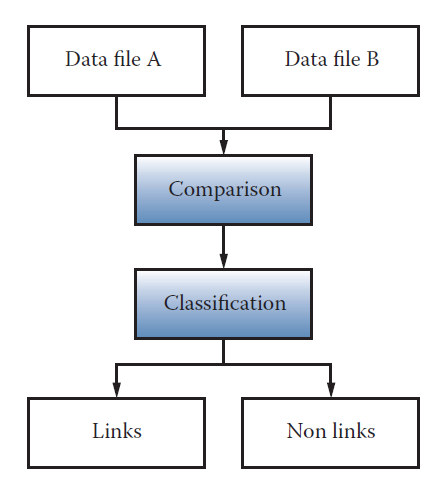
\includegraphics{images/bd1.png}
\caption{Pre-procesamiento}
\end{figure}

\begin{itemize}
\tightlist
\item
  Matching: Une información a partir de una clave, existen muchos problemas con claves tipo texto.
\item
  Aproximaciones a reglas para hacer math: Definir criterios para posibilitar el match basados en reglas, distancias cercanas, etc.
\item
  Match basados en probabilidad: Fellegi--Sunter method
\end{itemize}

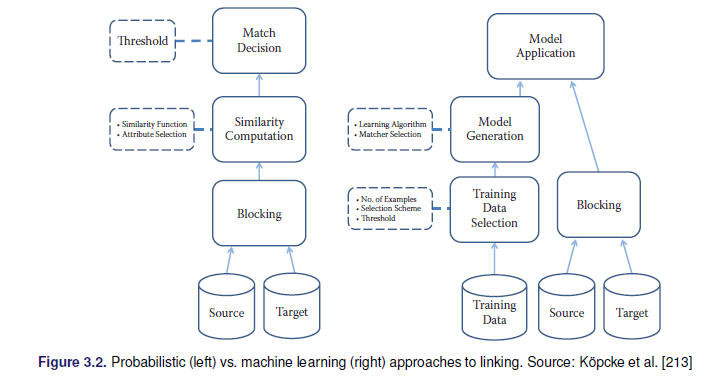
\includegraphics{images/bd2.PNG}

\hypertarget{bases-de-datos-1}{%
\subsection{Bases de datos}\label{bases-de-datos-1}}

Una vez que los datos fueron recolectados y enlazados entre diferentes fuentes, es necesario guardar la información. Ahora se discute las alternativas para guardar la información.

\begin{itemize}
\tightlist
\item
  DBMS (databasemanagement systems) Sistema de gestión de base de datos: Decidir que herramienta usar segun la dimensión de los archivos.
\end{itemize}

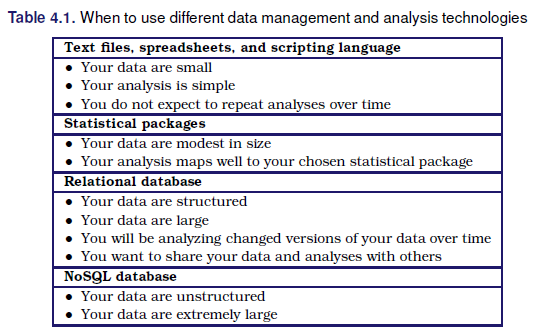
\includegraphics{images/bd3.PNG}

\begin{itemize}
\tightlist
\item
  Bases de datos espaciales
\item
  Múltiples formatos: \url{https://juliael.carto.com/}
\end{itemize}

\hypertarget{programando-con-big-data}{%
\subsection{Programando con Big Data}\label{programando-con-big-data}}

\begin{itemize}
\tightlist
\item
  MapReduce: map, shuffle y reduce
\end{itemize}

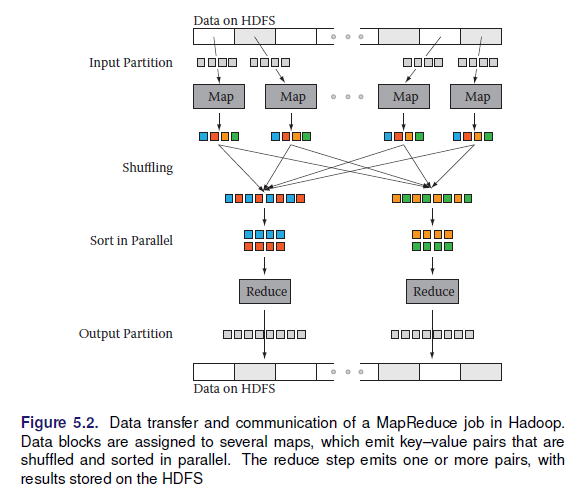
\includegraphics{images/bd5.PNG}

\begin{itemize}
\tightlist
\item
  Apache hadoop MapReduce (Hadoop Distributed File System HDFS)
\item
  Apache Spark
\end{itemize}

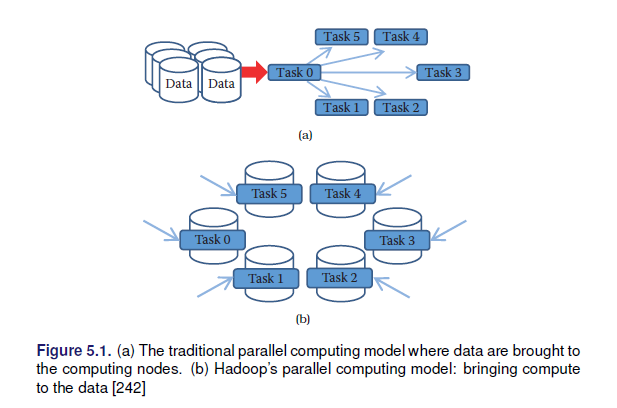
\includegraphics{images/bd4.PNG}

\hypertarget{anuxe1lisis-y-modelado}{%
\section{Análisis y modelado}\label{anuxe1lisis-y-modelado}}

\hypertarget{machine-learning}{%
\subsection{Machine learning}\label{machine-learning}}

\textbf{¿Machine learning = Statistics?}

Verán que muchos métodos discutidos a lo largo de su formación como estadísticos aparecen dentro del maching learning y que son llamados con otros nombres.

Al pensar en machine learning debemos asociarlo directamente con procesos computacionales, muchos otros conceptos giran al rededor de esta idea como la inteligencia artificial. Proceso de machine learning hoy:

\begin{itemize}
\tightlist
\item
  Permiten manejar autos de forma autónoma
\item
  Puede recomendar libros, amistades, música, etc
\item
  Identificar drogas, proteínas y ciertos génes
\item
  Se usa para detectar ciertos tipos de cáncer y otras enfermedades médicas
\item
  Ayudan a conocer que estudiantes necesitan un apoyo adicional
\item
  Ayudan a persuadir por que candidato votar en las elecciones.
\end{itemize}

\hypertarget{el-proceso-del-machine-learning}{%
\subsubsection{El proceso del machine learning}\label{el-proceso-del-machine-learning}}

\begin{itemize}
\tightlist
\item
  Entender el problema y la meta
\item
  Formular esto como un problema de machine learning
\item
  Explorar y preparar los datos
\item
  Feature engineeing
\item
  Selección del método
\item
  Evaluación
\item
  Deployment
\end{itemize}

\hypertarget{formulaciuxf3n-del-problema}{%
\subsubsection{Formulación del problema}\label{formulaciuxf3n-del-problema}}

En ML existen 2 grandes categorías

\begin{enumerate}
\def\labelenumi{\arabic{enumi}.}
\item
  Aprendizaje supervisado: Existe una \(Y\) que queremos predecir o clasificar a partir de los datos. El fin es el ajuste y la generalización
  * Clasificación (\(Y\) cualitativa)
  * Predicción
  * Regresión (\(Y\) cuantitativa)
\item
  Aprendizaje no supervisado: No existe una variable objetivo, se quiere conocer, entender las asociaciones y patrones naturales en los datos.
  * Clustering
  * PCA, MCA
\end{enumerate}

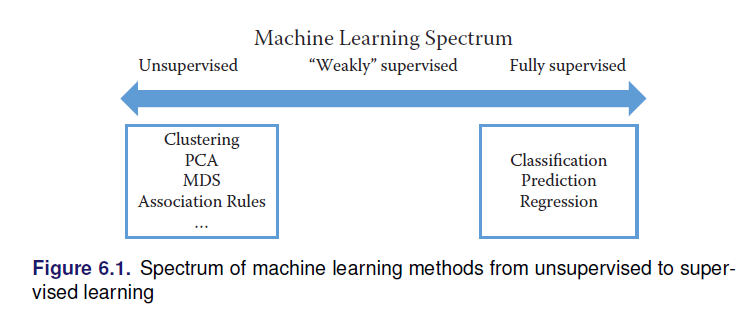
\includegraphics{images/bd6.PNG}

\hypertarget{anuxe1lisis-de-texto-entendiendo-lo-que-la-gente-escribe}{%
\subsection{Análisis de texto: Entendiendo lo que la gente escribe}\label{anuxe1lisis-de-texto-entendiendo-lo-que-la-gente-escribe}}

\begin{itemize}
\tightlist
\item
  Clasificación de documentos
\item
  Análisis de sentimientos
\item
  Etiquetado de discursos
\end{itemize}

\hypertarget{networks}{%
\subsection{Networks}\label{networks}}

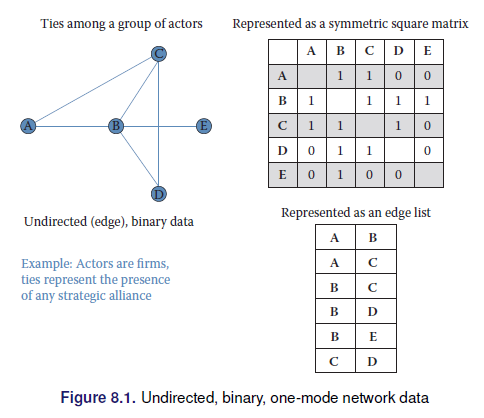
\includegraphics{images/bd7.PNG}
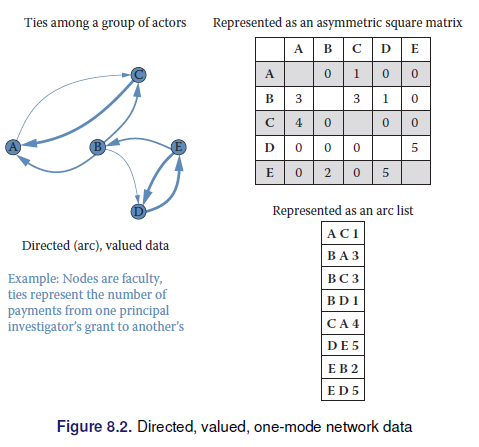
\includegraphics{images/bd8.PNG}

\hypertarget{inferencia-y-uxe9tica}{%
\section{Inferencia y ética}\label{inferencia-y-uxe9tica}}

\hypertarget{informaciuxf3n-y-visualizaciuxf3n}{%
\subsection{Información y visualización}\label{informaciuxf3n-y-visualizaciuxf3n}}

\begin{quote}
Los usuarios pueden escanear, reconocer, comprender y recordar representaciones visualmente estructuradas más rápidamente de lo que pueden procesar representaciones no estructuradas
\end{quote}

\begin{quote}
La ciencia de la visualización se basa en múltiples campos, como la psicología perceptiva, las estadísticas y el diseño gráfico para presentar información
\end{quote}

\begin{quote}
La efectividad de una visualización depende tanto de las necesidades de análisis como de los objetivos de diseño.
\end{quote}

\begin{quote}
El diseño, el desarrollo y la evaluación de una visualización se guían por la comprensión de los antecedentes y las metas del público objetivo.
\end{quote}

El desarrollo de una visualización efectiva es un proceso iterativo que generalmente incluye los siguientes pasos:

\begin{itemize}
\tightlist
\item
  Especificar las necesidades del usuario, tareas, requisitos de accesibilidad y criterios para el éxito.
\item
  Preparar datos (limpiar, transformar).
\item
  Diseñar representaciones visuales.
\item
  Interacción de diseño.
\item
  Planifique el intercambio de ideas, procedencia.
\item
  Prototipo / evaluación, incluidas las pruebas de usabilidad.
\item
  Implementar (supervisar el uso, proporcionar soporte al usuario, gestionar el proceso de revisión).
\end{itemize}

\includegraphics{https://www.babynamewizard.com/voyager}

\hypertarget{dashboards}{%
\subsubsection{Dashboards}\label{dashboards}}

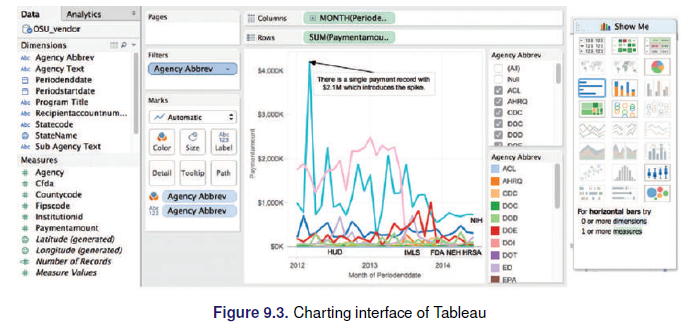
\includegraphics{images/bd9.PNG}
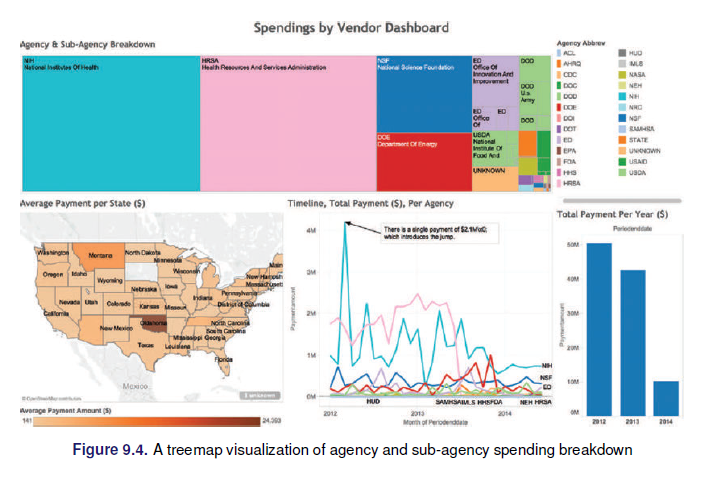
\includegraphics{images/bd10.PNG}

\hypertarget{elementos}{%
\subsubsection{Elementos}\label{elementos}}

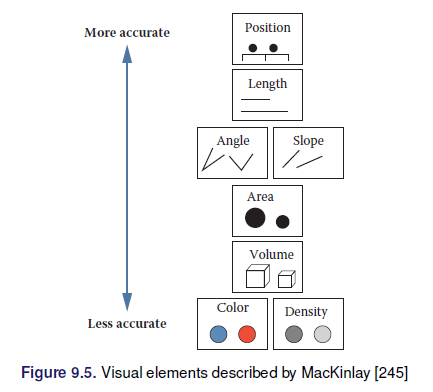
\includegraphics{images/bd11.PNG}

\hypertarget{datos-espaciales}{%
\subsubsection{Datos espaciales}\label{datos-espaciales}}

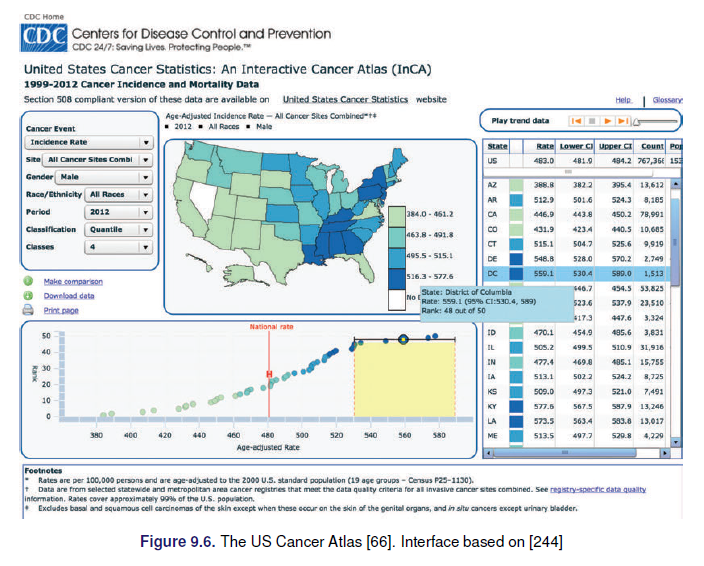
\includegraphics{images/bd12.PNG}

\begin{itemize}
\tightlist
\item
  Datos temporales
\item
  Datos jerarquicos
\item
  Datos de redes
\item
  Datos de texto
\end{itemize}

Tarea: resumir los siguientes puntos del libro: Big Data and Social Science, Ian Foster.

\hypertarget{error-e-inferencia}{%
\subsection{Error e inferencia}\label{error-e-inferencia}}

\hypertarget{privacidad-y-confidencialidad}{%
\subsection{Privacidad y confidencialidad}\label{privacidad-y-confidencialidad}}

\hypertarget{workbooks}{%
\subsection{Workbooks}\label{workbooks}}

\hypertarget{ejercicios-propuestos-1}{%
\section{Ejercicios Propuestos}\label{ejercicios-propuestos-1}}

\begin{enumerate}
\def\labelenumi{\arabic{enumi}.}
\tightlist
\item
  Explorar los métodos cuasi-experimentales que existen
\item
  Buscar informacion respecto a: los matriculados en educacion regular y universidad por año y departamento en Bolivia
\item
  Empleando la fuente anterior, generar en R el có
  digo que cargue el archivo encontrado
\item
  Buscar dos papers (1) donde se uso machine learning y (2) análisis de texto y comentar con al menos 5000 caractéres
\item
  Buscar ejemplos (al menos uno) de bases de datos, páginas web u otros asociados a datos que no respeten los principios de privacidad y confidencialidad.
\end{enumerate}

\hypertarget{refs}{}
\leavevmode\hypertarget{ref-R-rmarkdown}{}%
Allaire, JJ, Yihui Xie, Jonathan McPherson, Javier Luraschi, Kevin Ushey, Aron Atkins, Hadley Wickham, Joe Cheng, Winston Chang, and Richard Iannone. 2020. \emph{Rmarkdown: Dynamic Documents for R}. \url{https://CRAN.R-project.org/package=rmarkdown}.

\leavevmode\hypertarget{ref-R-base}{}%
R Core Team. 2019. \emph{R: A Language and Environment for Statistical Computing}. Vienna, Austria: R Foundation for Statistical Computing. \url{https://www.R-project.org/}.

\leavevmode\hypertarget{ref-R-knitr}{}%
Xie, Yihui. 2019. \emph{Knitr: A General-Purpose Package for Dynamic Report Generation in R}. \url{https://CRAN.R-project.org/package=knitr}.

\leavevmode\hypertarget{ref-R-bookdown}{}%
---------. 2020. \emph{Bookdown: Authoring Books and Technical Documents with R Markdown}. \url{https://CRAN.R-project.org/package=bookdown}.

\leavevmode\hypertarget{ref-Xie2018}{}%
Xie, Yihui, J. J. Allaire, and Garrett Grolemund. 2018. ``How to Read This Book.'' \emph{Transforming Climate Finance and Green Investment with Blockchains}, 1. \url{https://doi.org/10.1016/b978-0-12-814447-3.00041-0}.

\end{document}
